\documentclass{beamer}
\usepackage{multicol}
\usepackage{graphicx}

\graphicspath{{images/}}
\usetheme{CambridgeUS}
\beamertemplatenavigationsymbolsempty

\title{The Star Method}
\author[Agbo, Burke, Mako, Vance]{Komi Agbo, Dalton Burke, Nick Mako, James Vance}
\institute[CU Denver]{University of Colorado Denver}
\date{Fall 2019}

\begin{document}
\maketitle

\begin{frame}{Overview}
	\begin{multicols}{2}
	\tableofcontents
	\end{multicols}
\end{frame}

\section{The Problem}
\begin{frame}{Sam's Hauling}
	What do they do?
	\begin{itemize}
		\item Provide roll off dumpsters of various sizes (cans)
		\item Customers 
		\begin{itemize}
			\item Delivery 
			\item Pickup 
			\item Switch 
		\end{itemize}
	\end{itemize}

	\begin{center}
	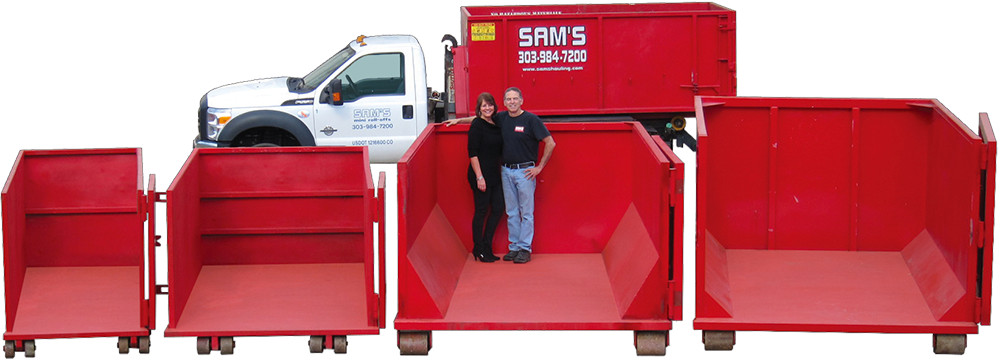
\includegraphics[width=7cm]{samshauling.jpg}
	\end{center}

\end{frame}
\begin{frame}{Sam's Hauling}
	How do they do it?
	\begin{itemize}
		\item Resources
			\begin{itemize}
				\item Cans
				\item Trucks
				\item Storage Yards
				\item Landfills
			\end{itemize}
		\item Constraints
			\begin{itemize}
				\item A truck can hold only one can
				\item Truck/Can/Location compatibility
				\item Can inventory at Storage Yards
				\item Customer time preference (AM/PM/None)
			\end{itemize}
	\end{itemize}
\end{frame}

\begin{frame}{Sam's Hauling}
	\begin{center}
	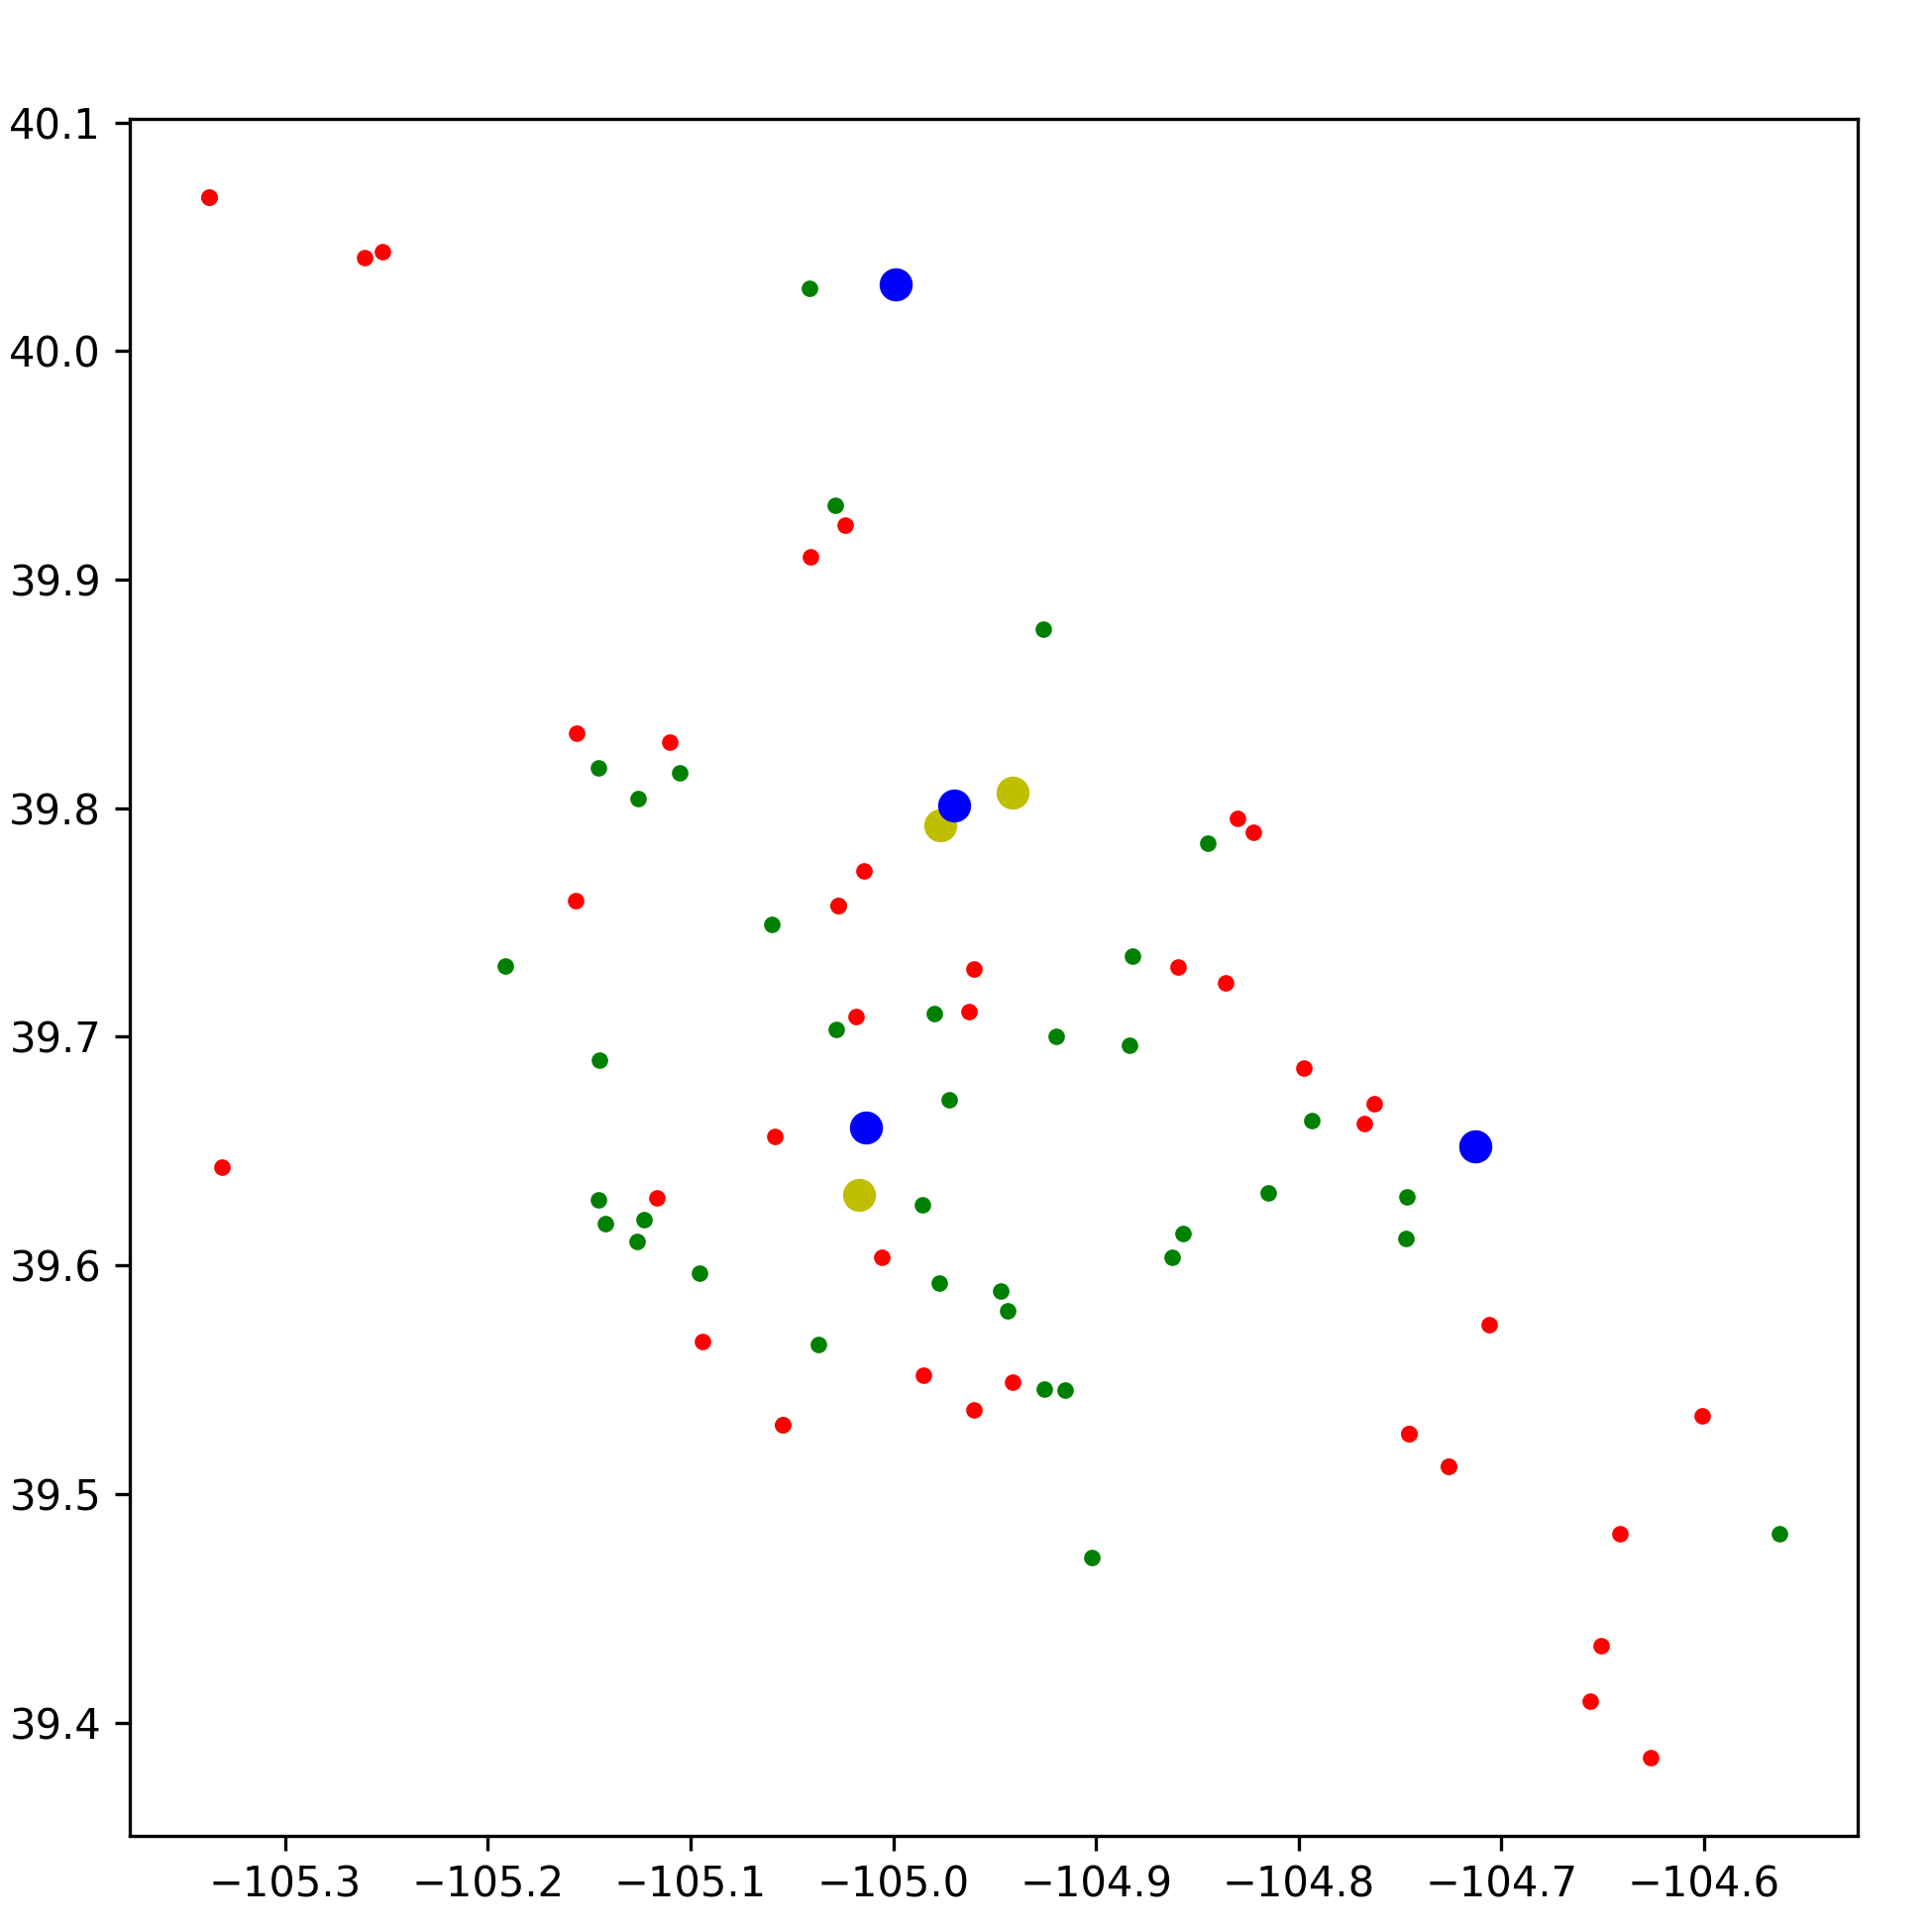
\includegraphics[width=7cm]{rawdata.png}\\
	Blue: Storage Yard, Yellow: Landfill, Green: Delivery, Red: Pickup.
	\end{center}
\end{frame}


\begin{frame}{Sam's Hauling}
	\begin{center}
	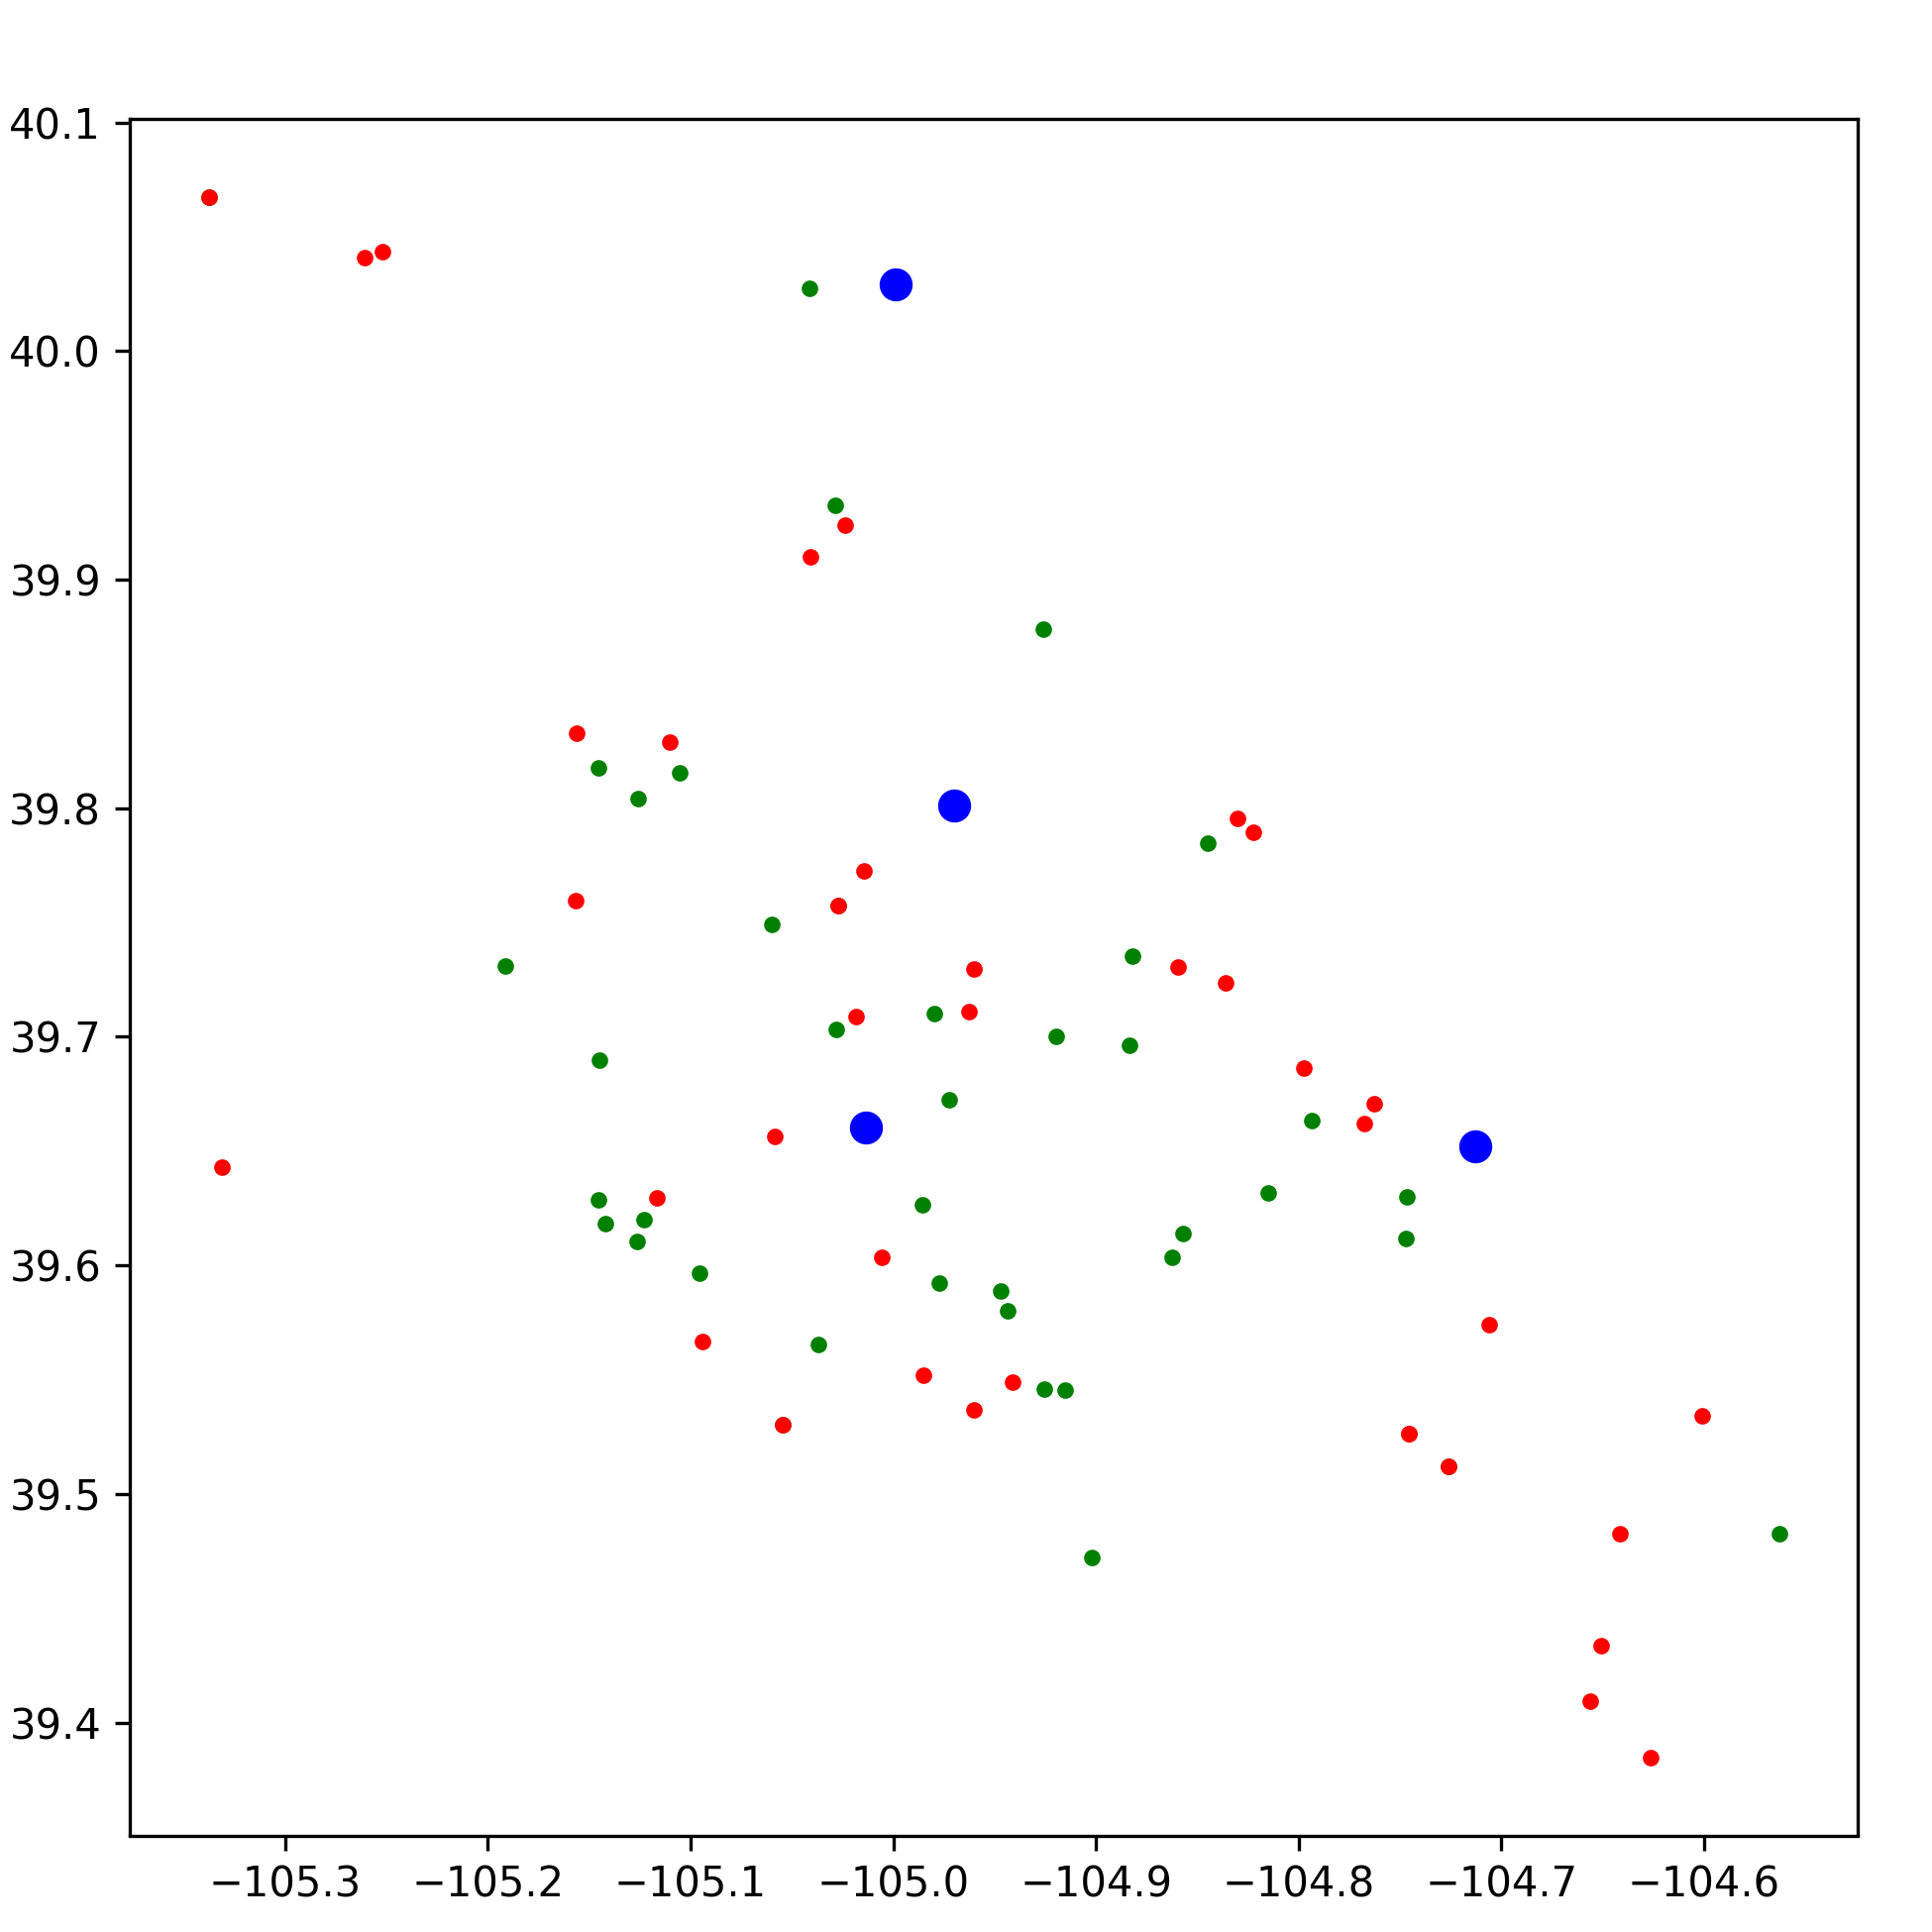
\includegraphics[width=7cm]{rawdata_nolf.png}\\
	Blue: Storage Yard, Green: Delivery, Red: Pickup.
	\end{center}
\end{frame}

\section{Stars}
\begin{frame}{Simplify}
	\begin{center}
	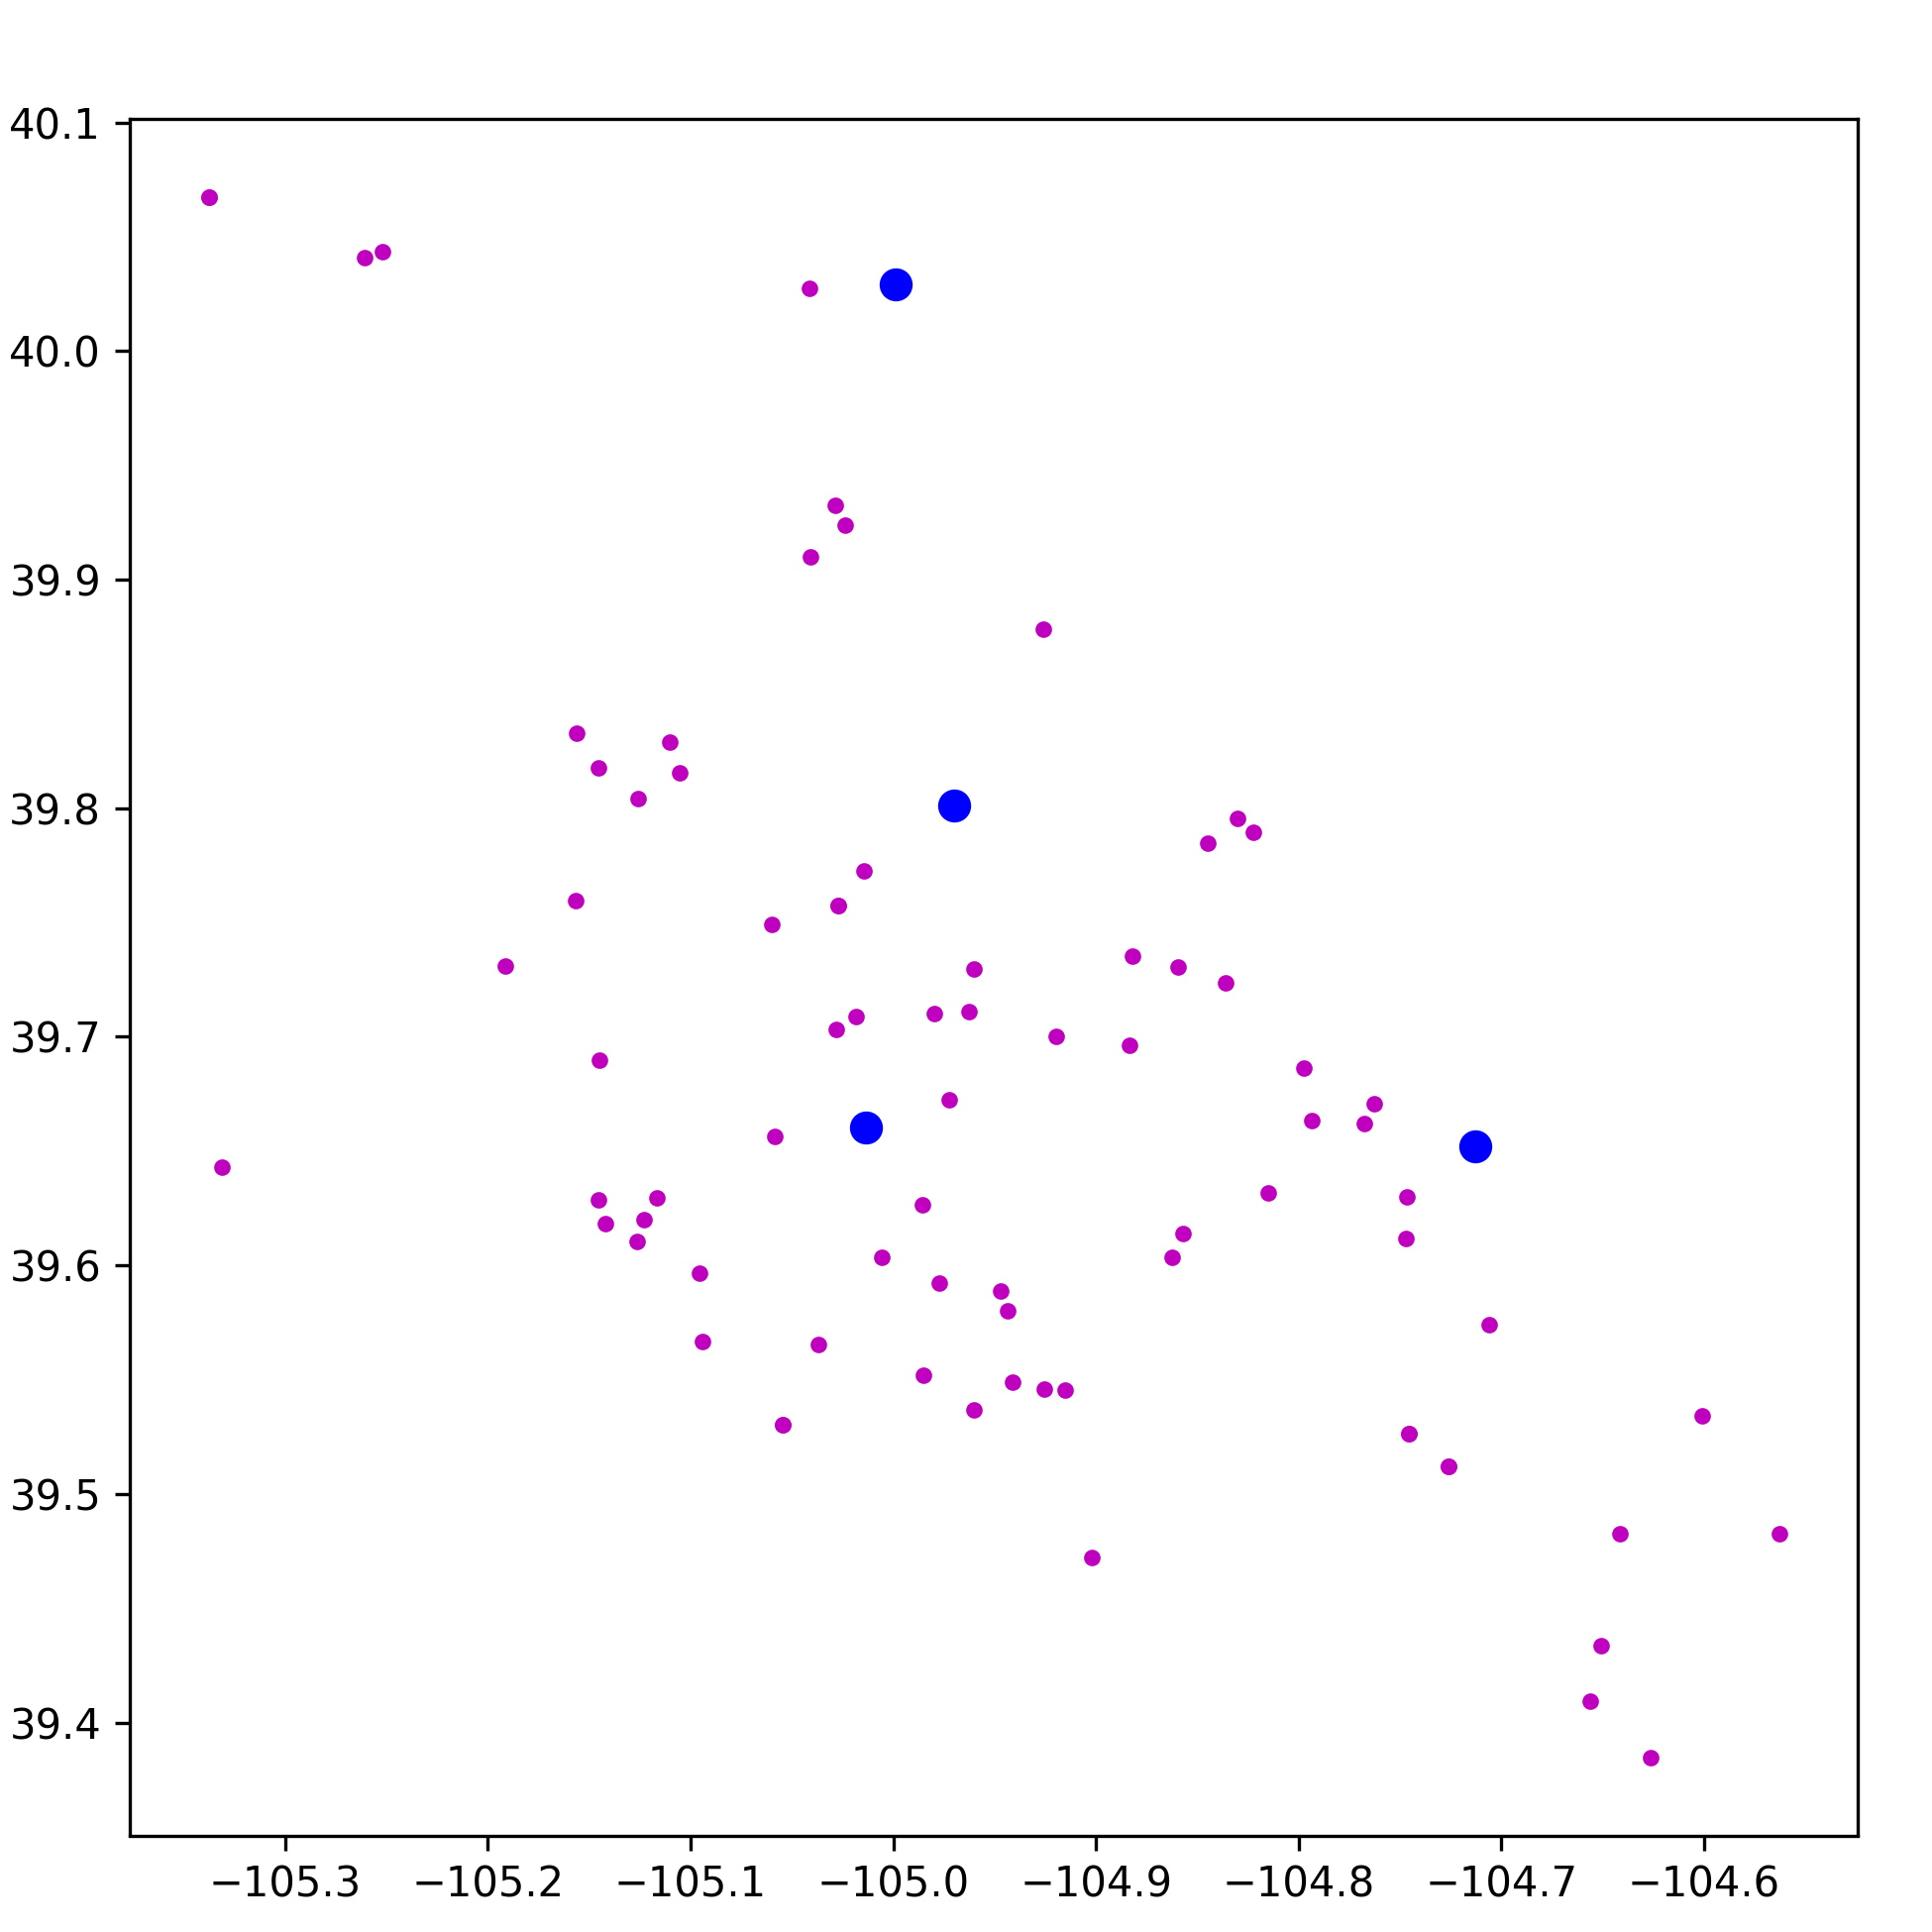
\includegraphics[width=7cm]{all_switch.png}\\
	What if they were all switches?
	\end{center}
\end{frame}

\begin{frame}{Simplify}
	\begin{center}
	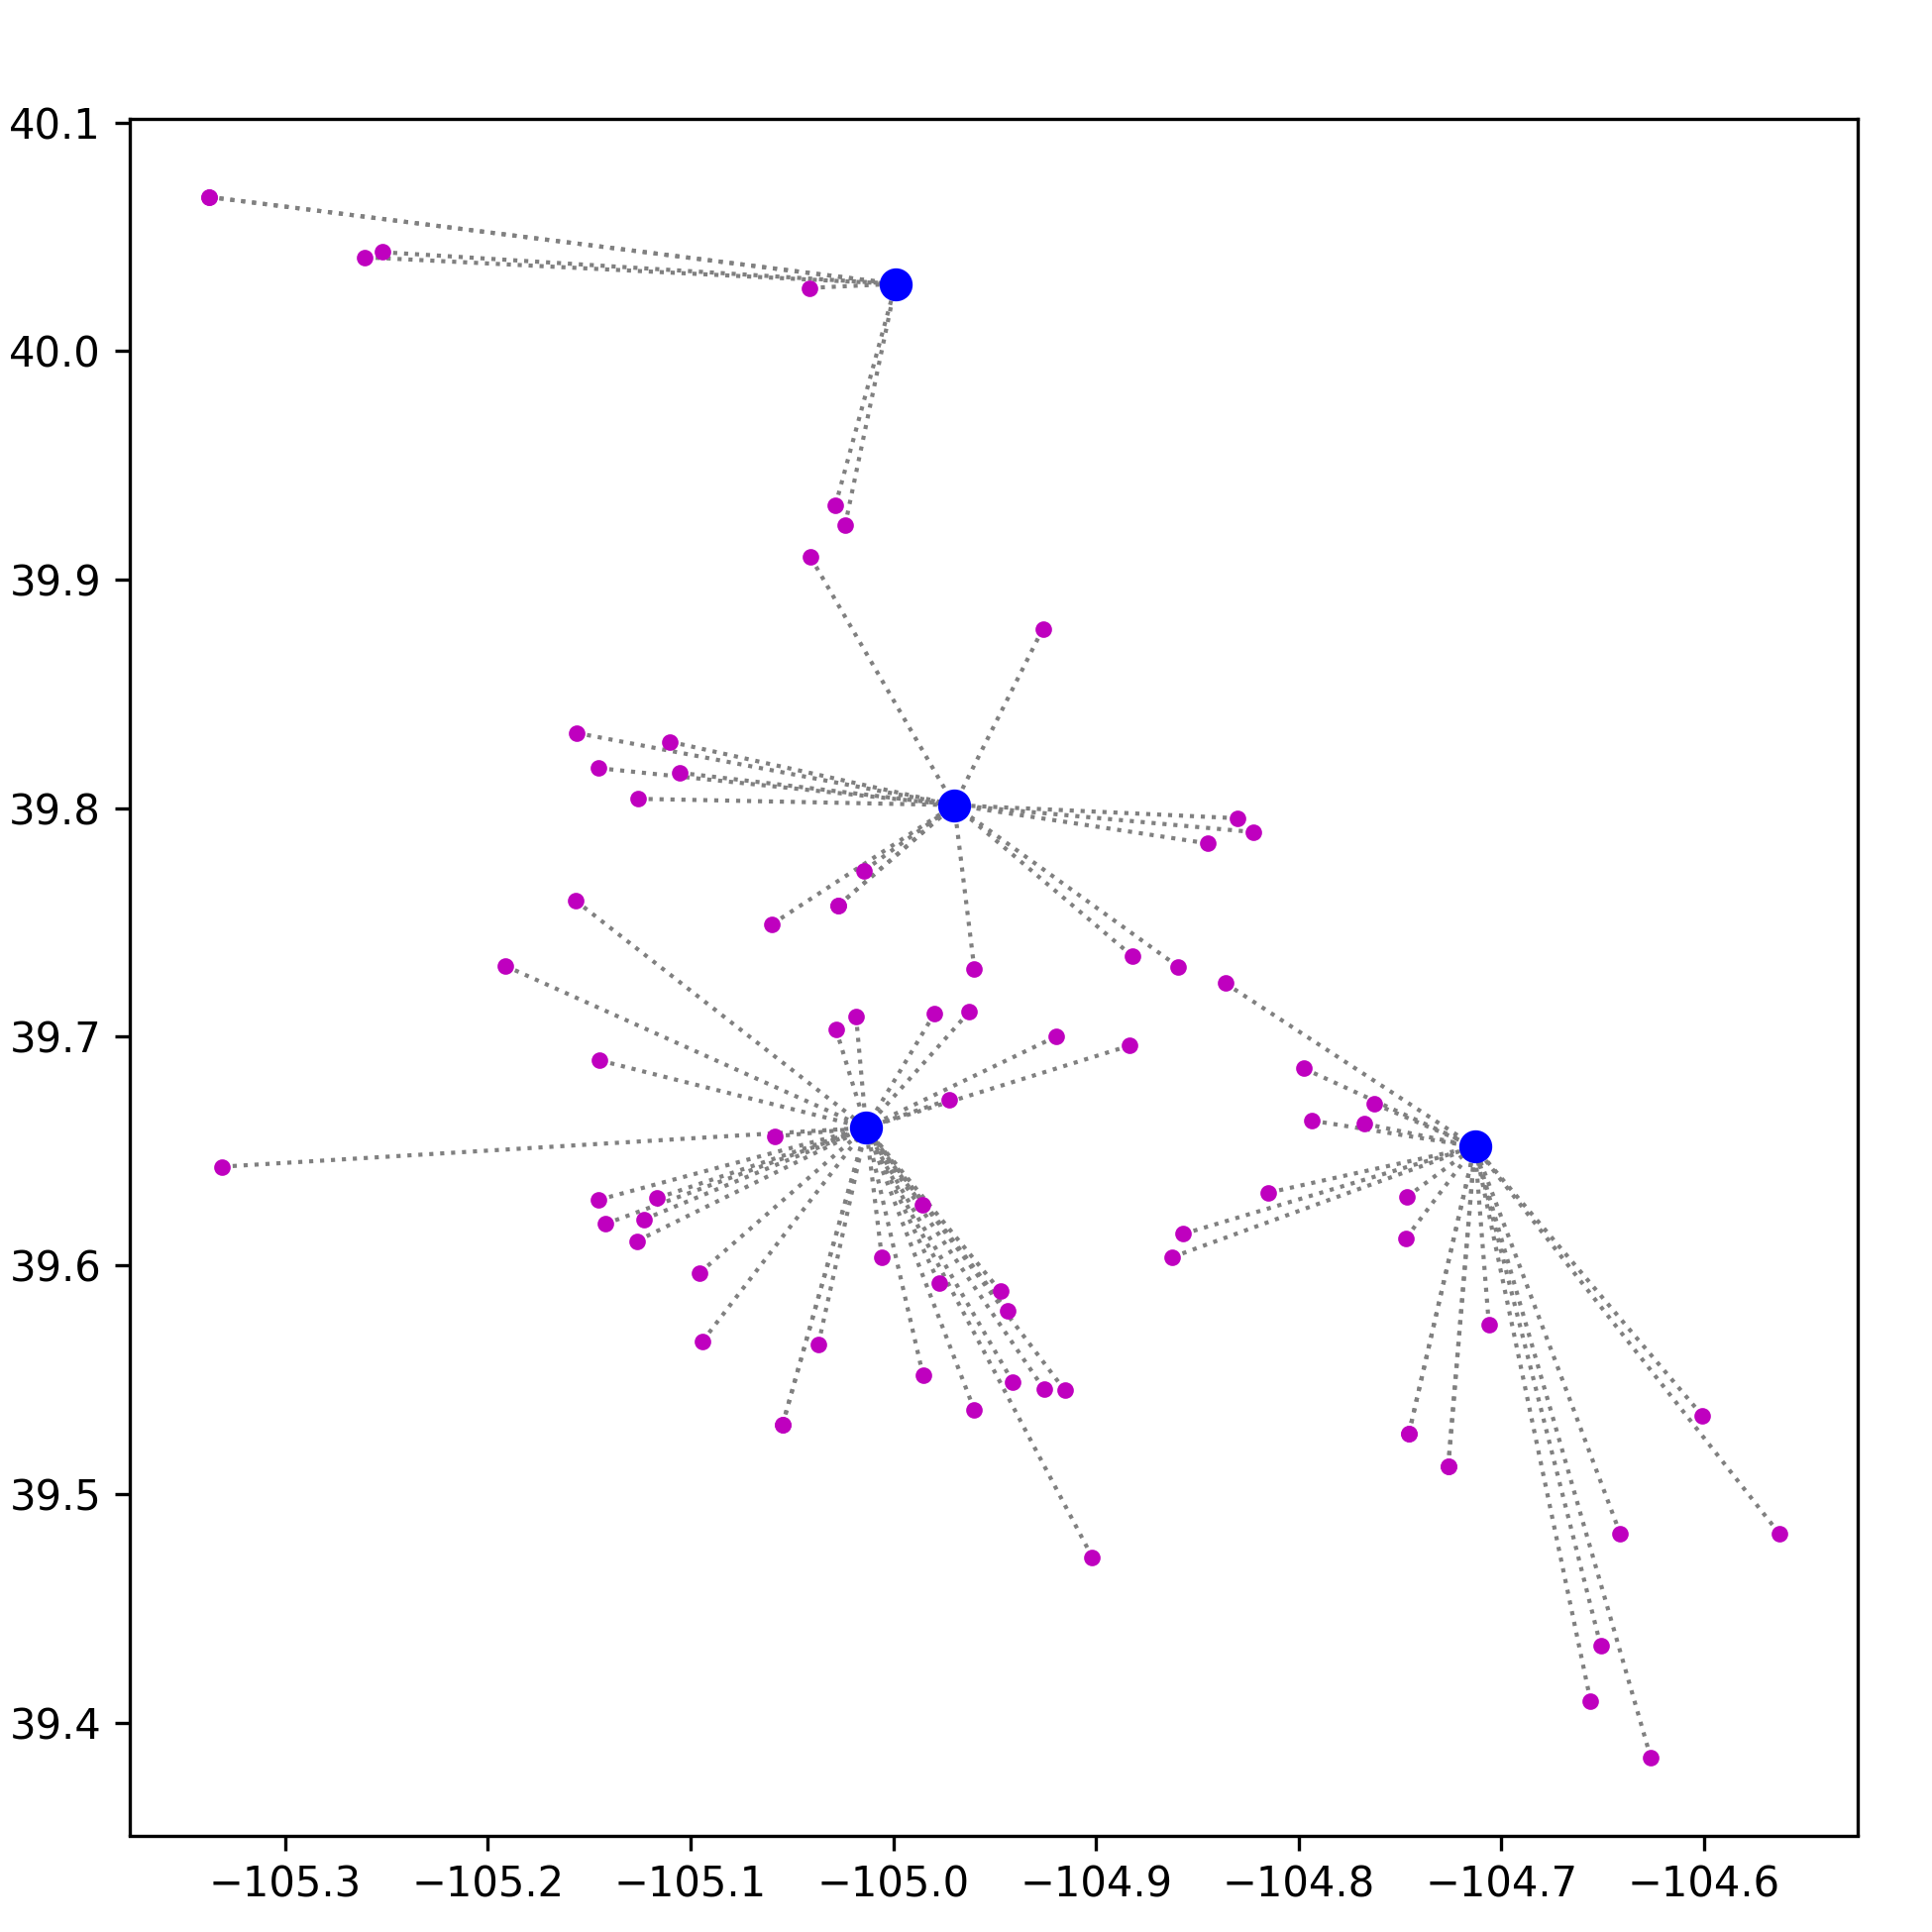
\includegraphics[width=7cm]{all_switch_star.png}\\
	Associate each with the nearest storage yard.
	\end{center}
\end{frame}


\begin{frame}{Simplify}
	\begin{center}
	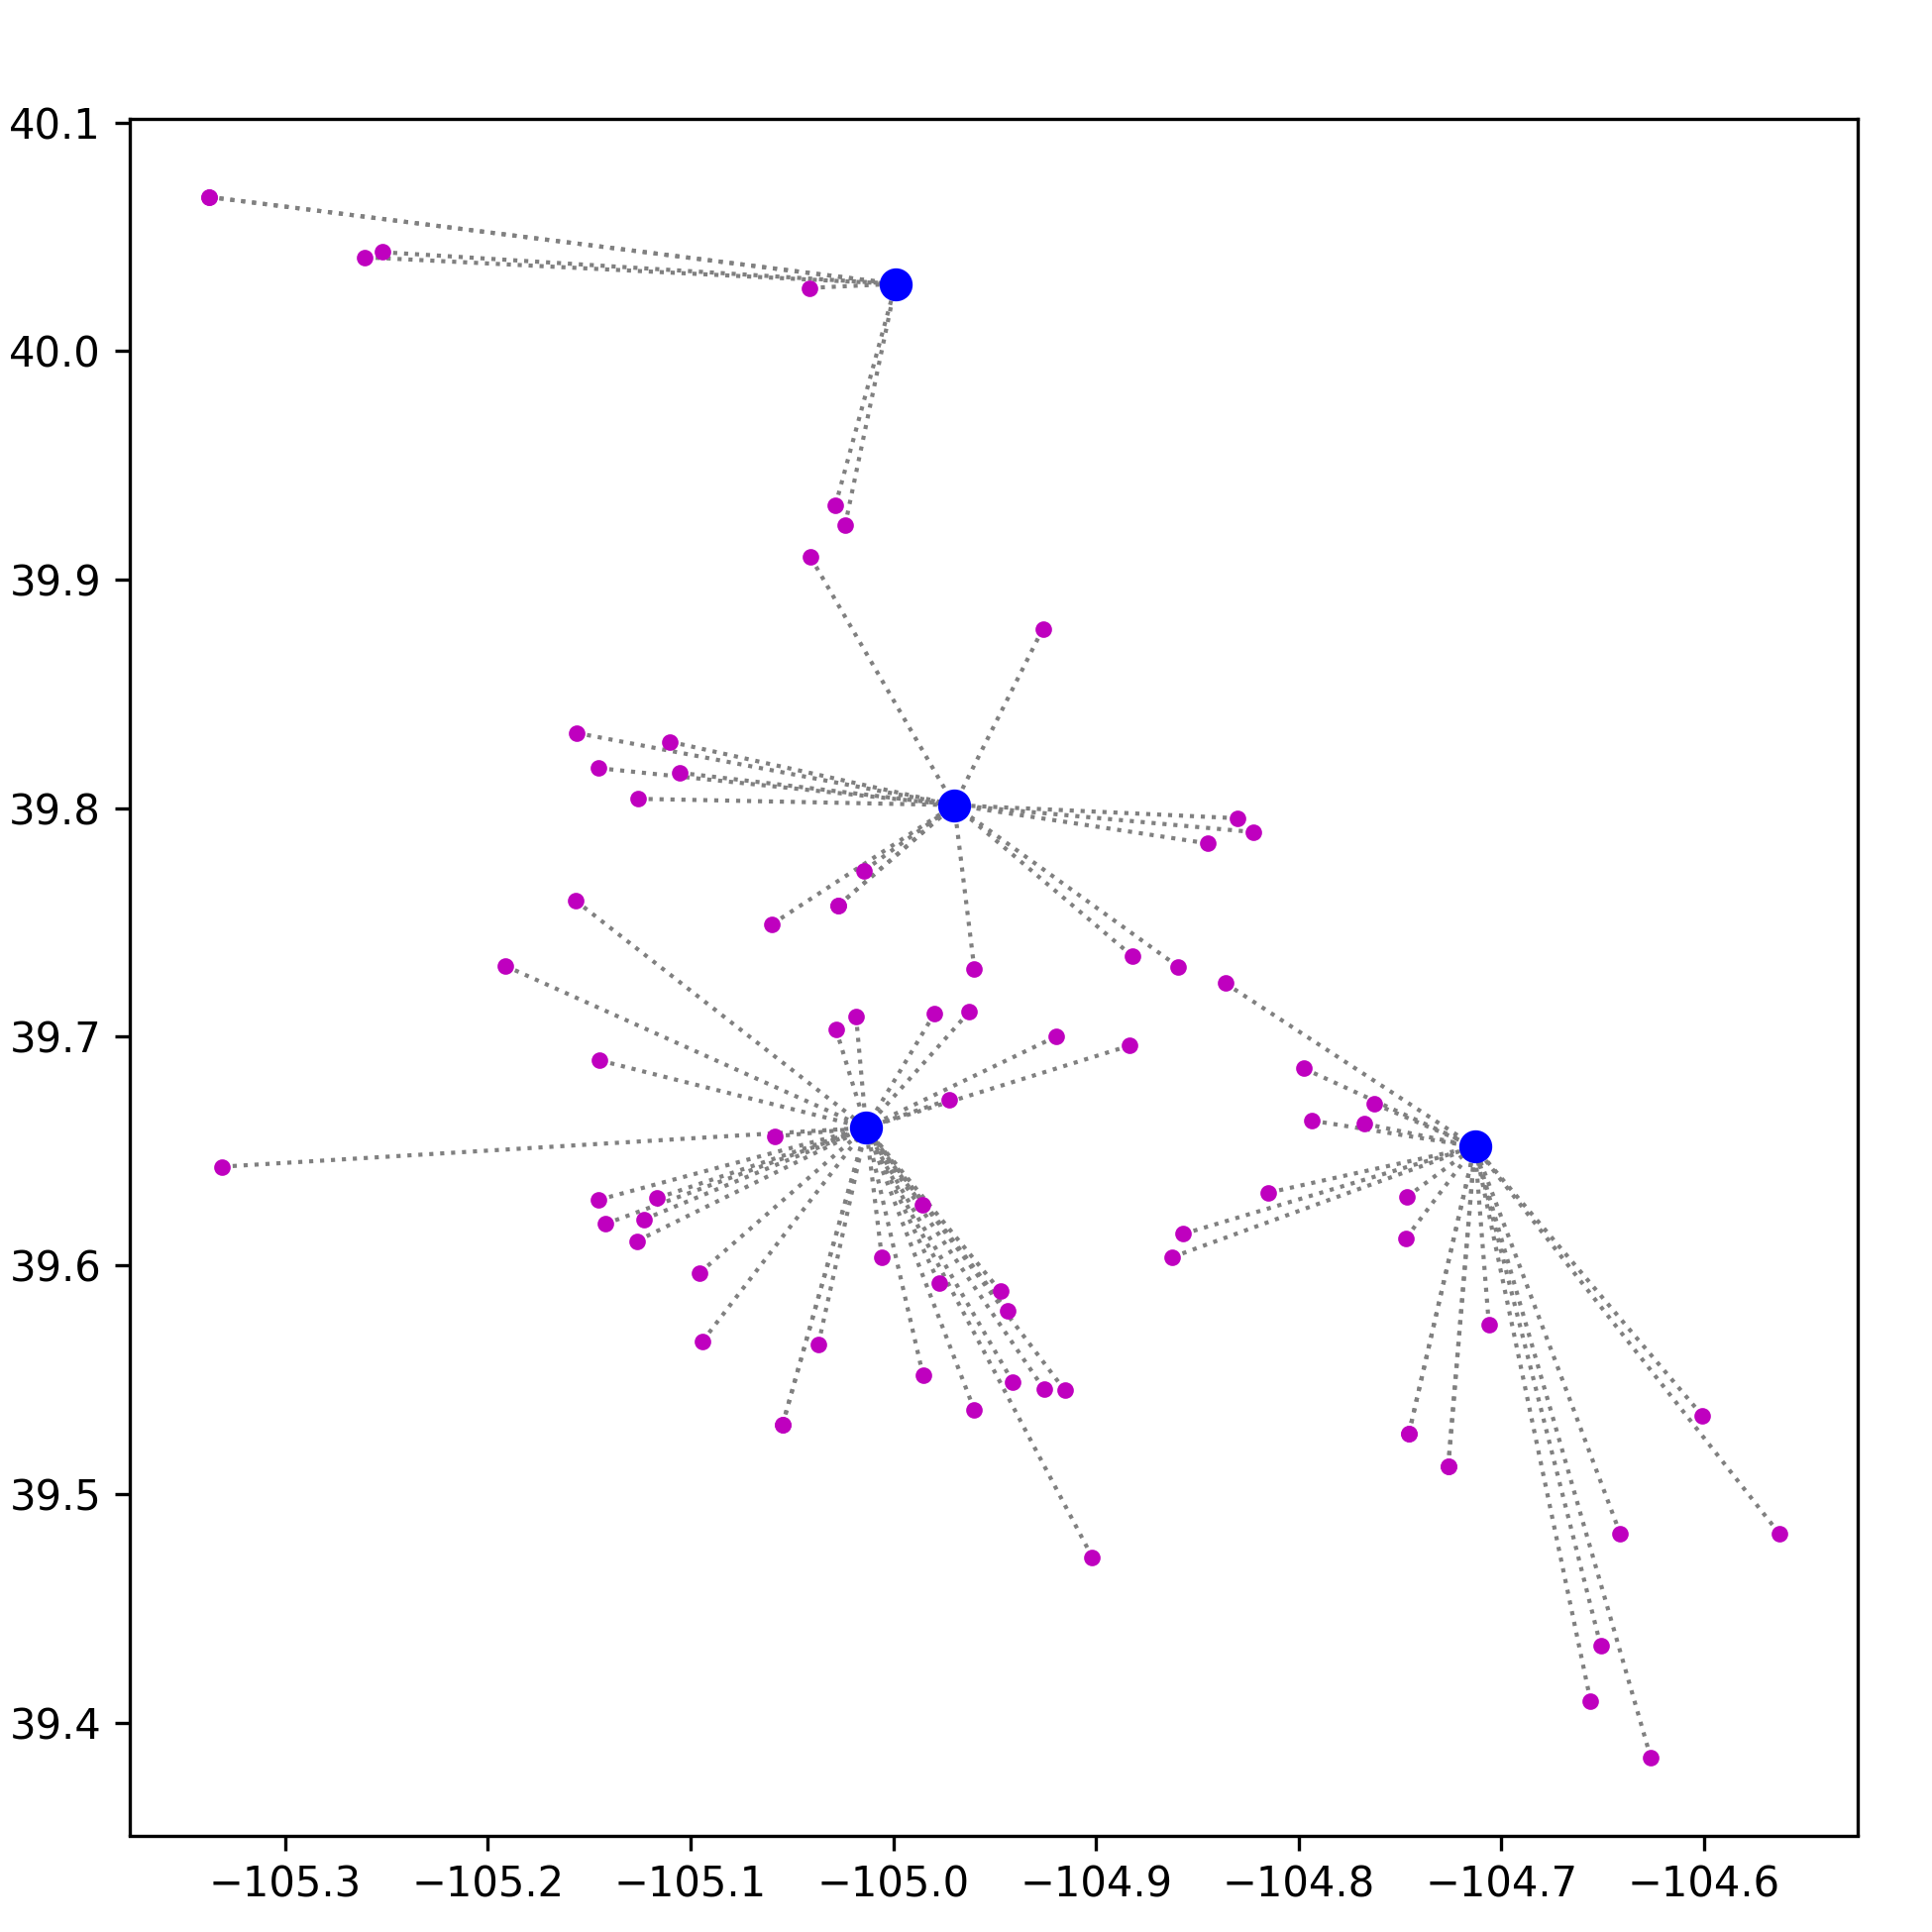
\includegraphics[width=7cm]{all_switch_star.png}\\
	Transitions will come later. For now, we will teleport.
	\end{center}
\end{frame}

\begin{frame}{Back to Reality}
	\begin{center}
	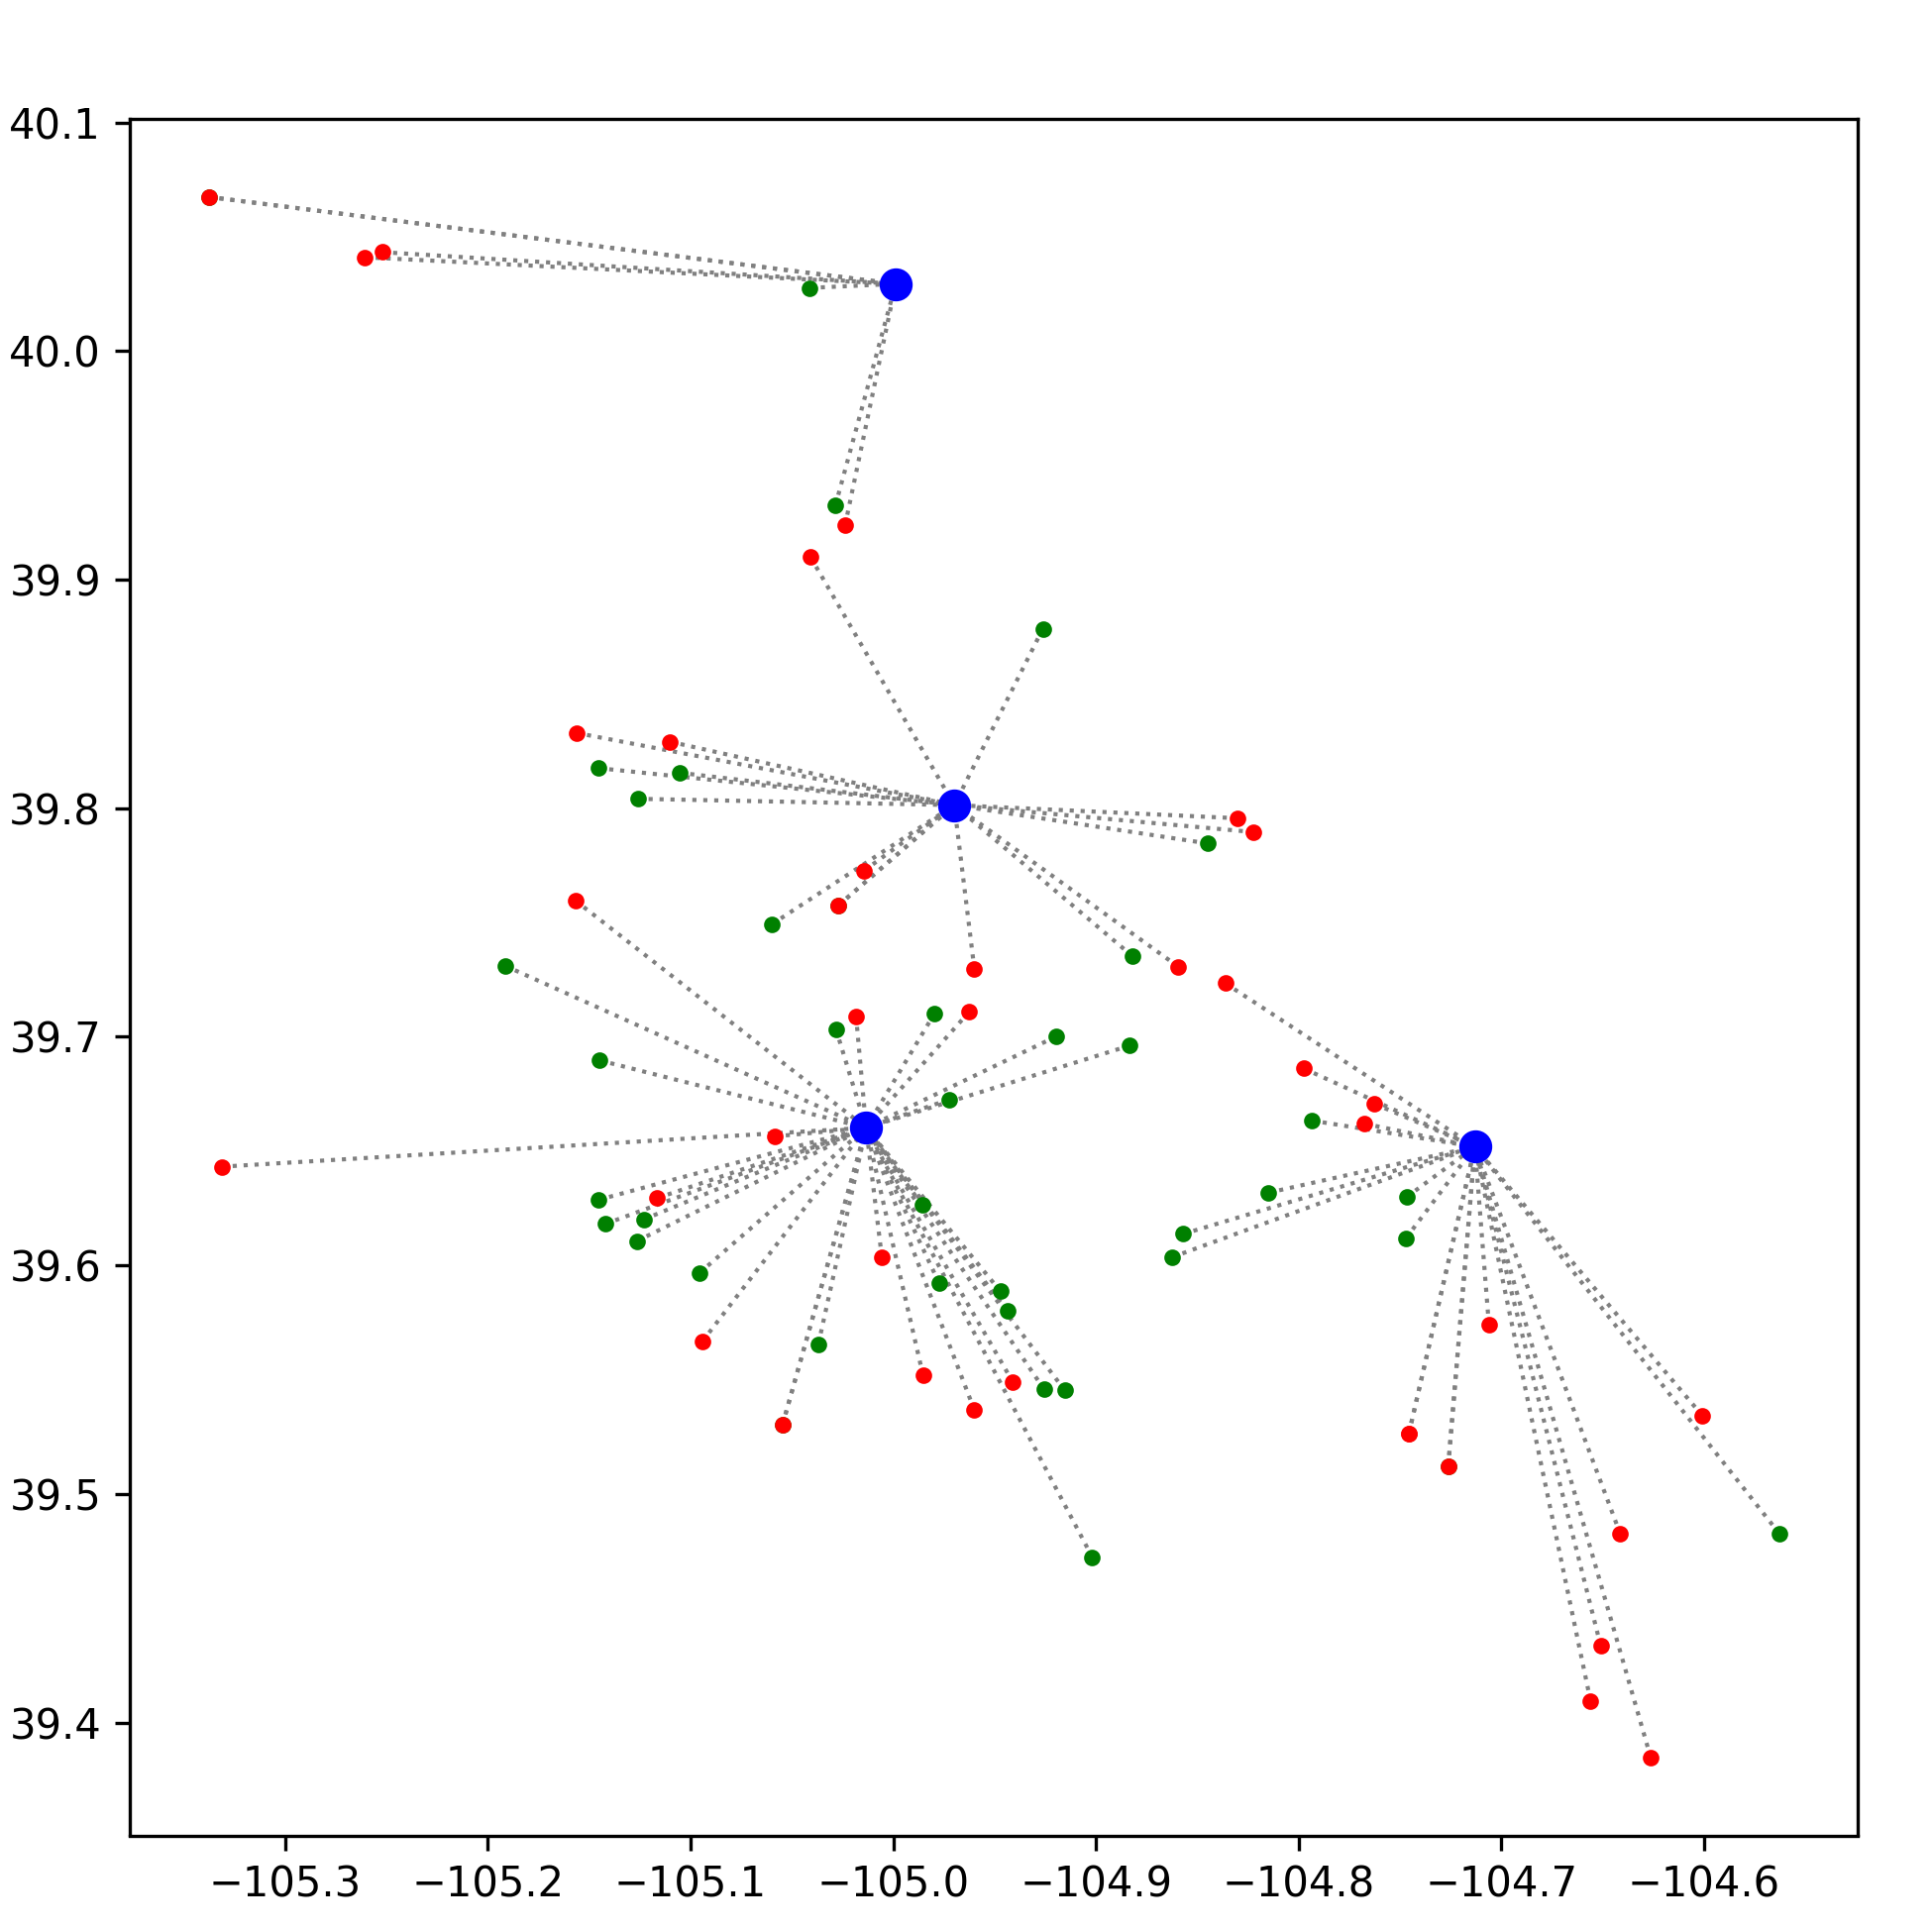
\includegraphics[width=7cm]{stars.png}\\
	Deliveries and Pickups
	\end{center}
\end{frame}

\begin{frame}{Back to Reality}
	\begin{center}
	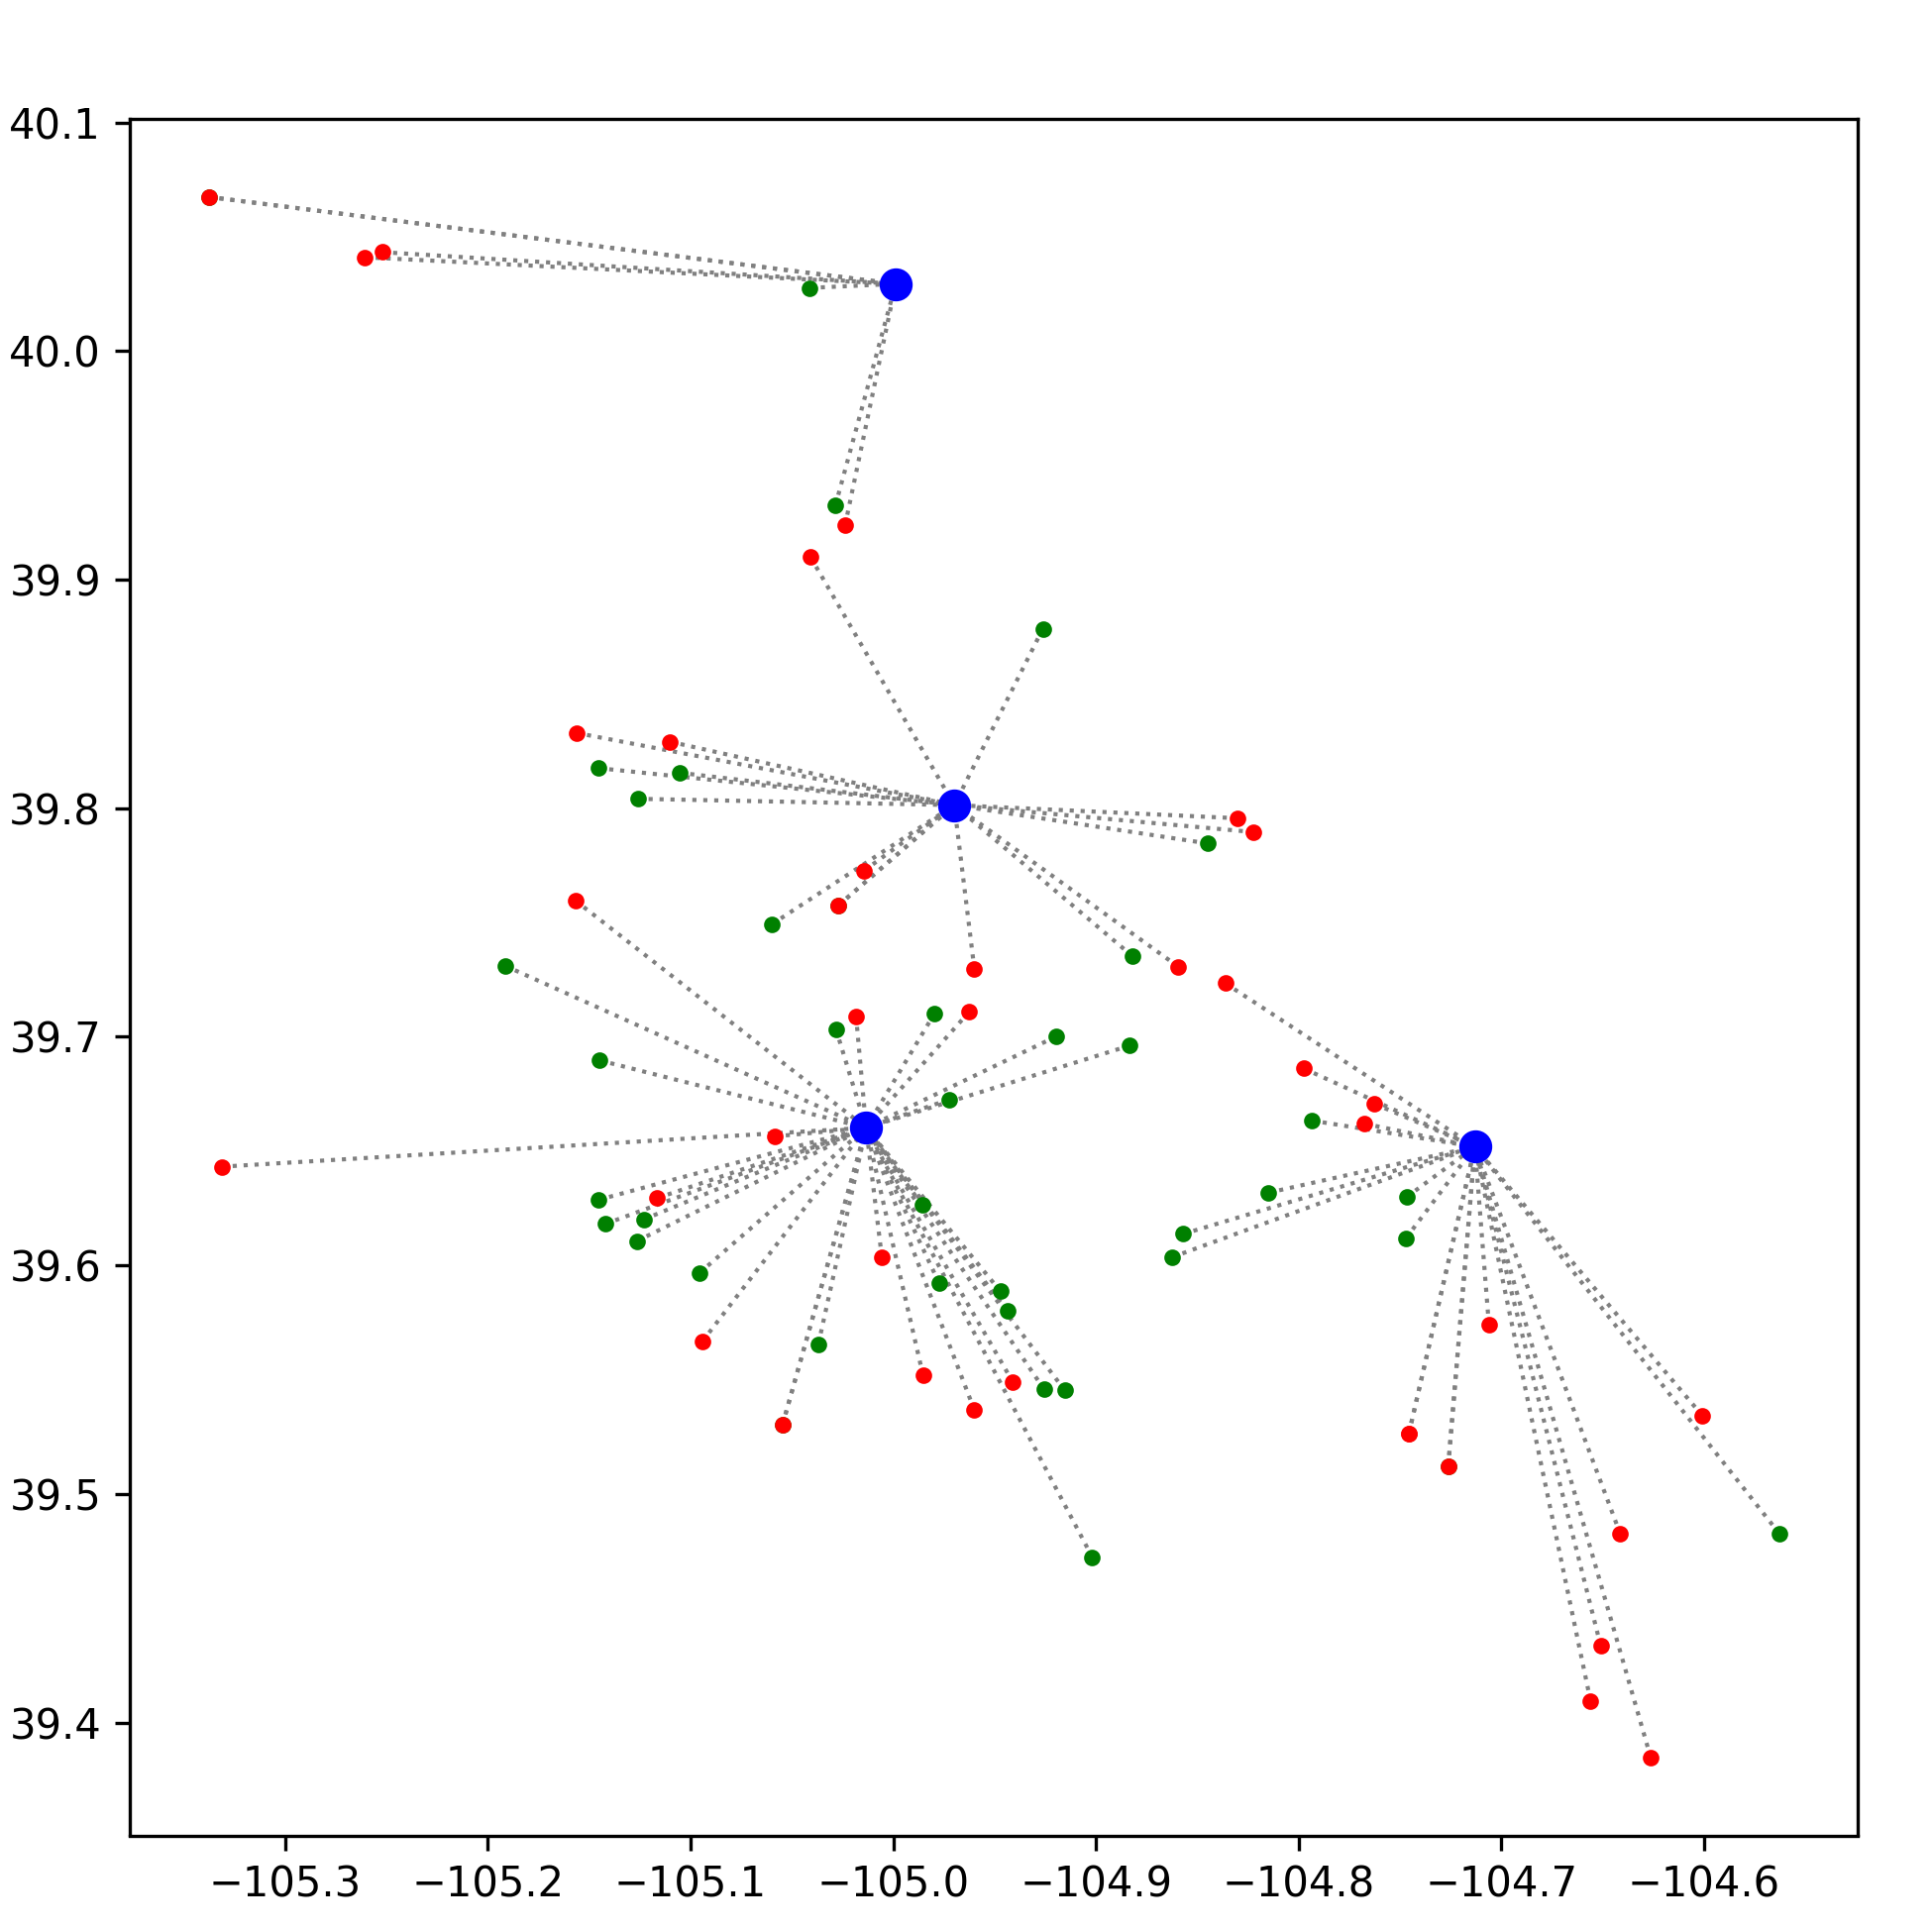
\includegraphics[width=7cm]{stars.png}\\
	After a delivery, the driver has an empty truck.
	\end{center}
\end{frame}

\begin{frame}{Back to Reality}
	\begin{center}
	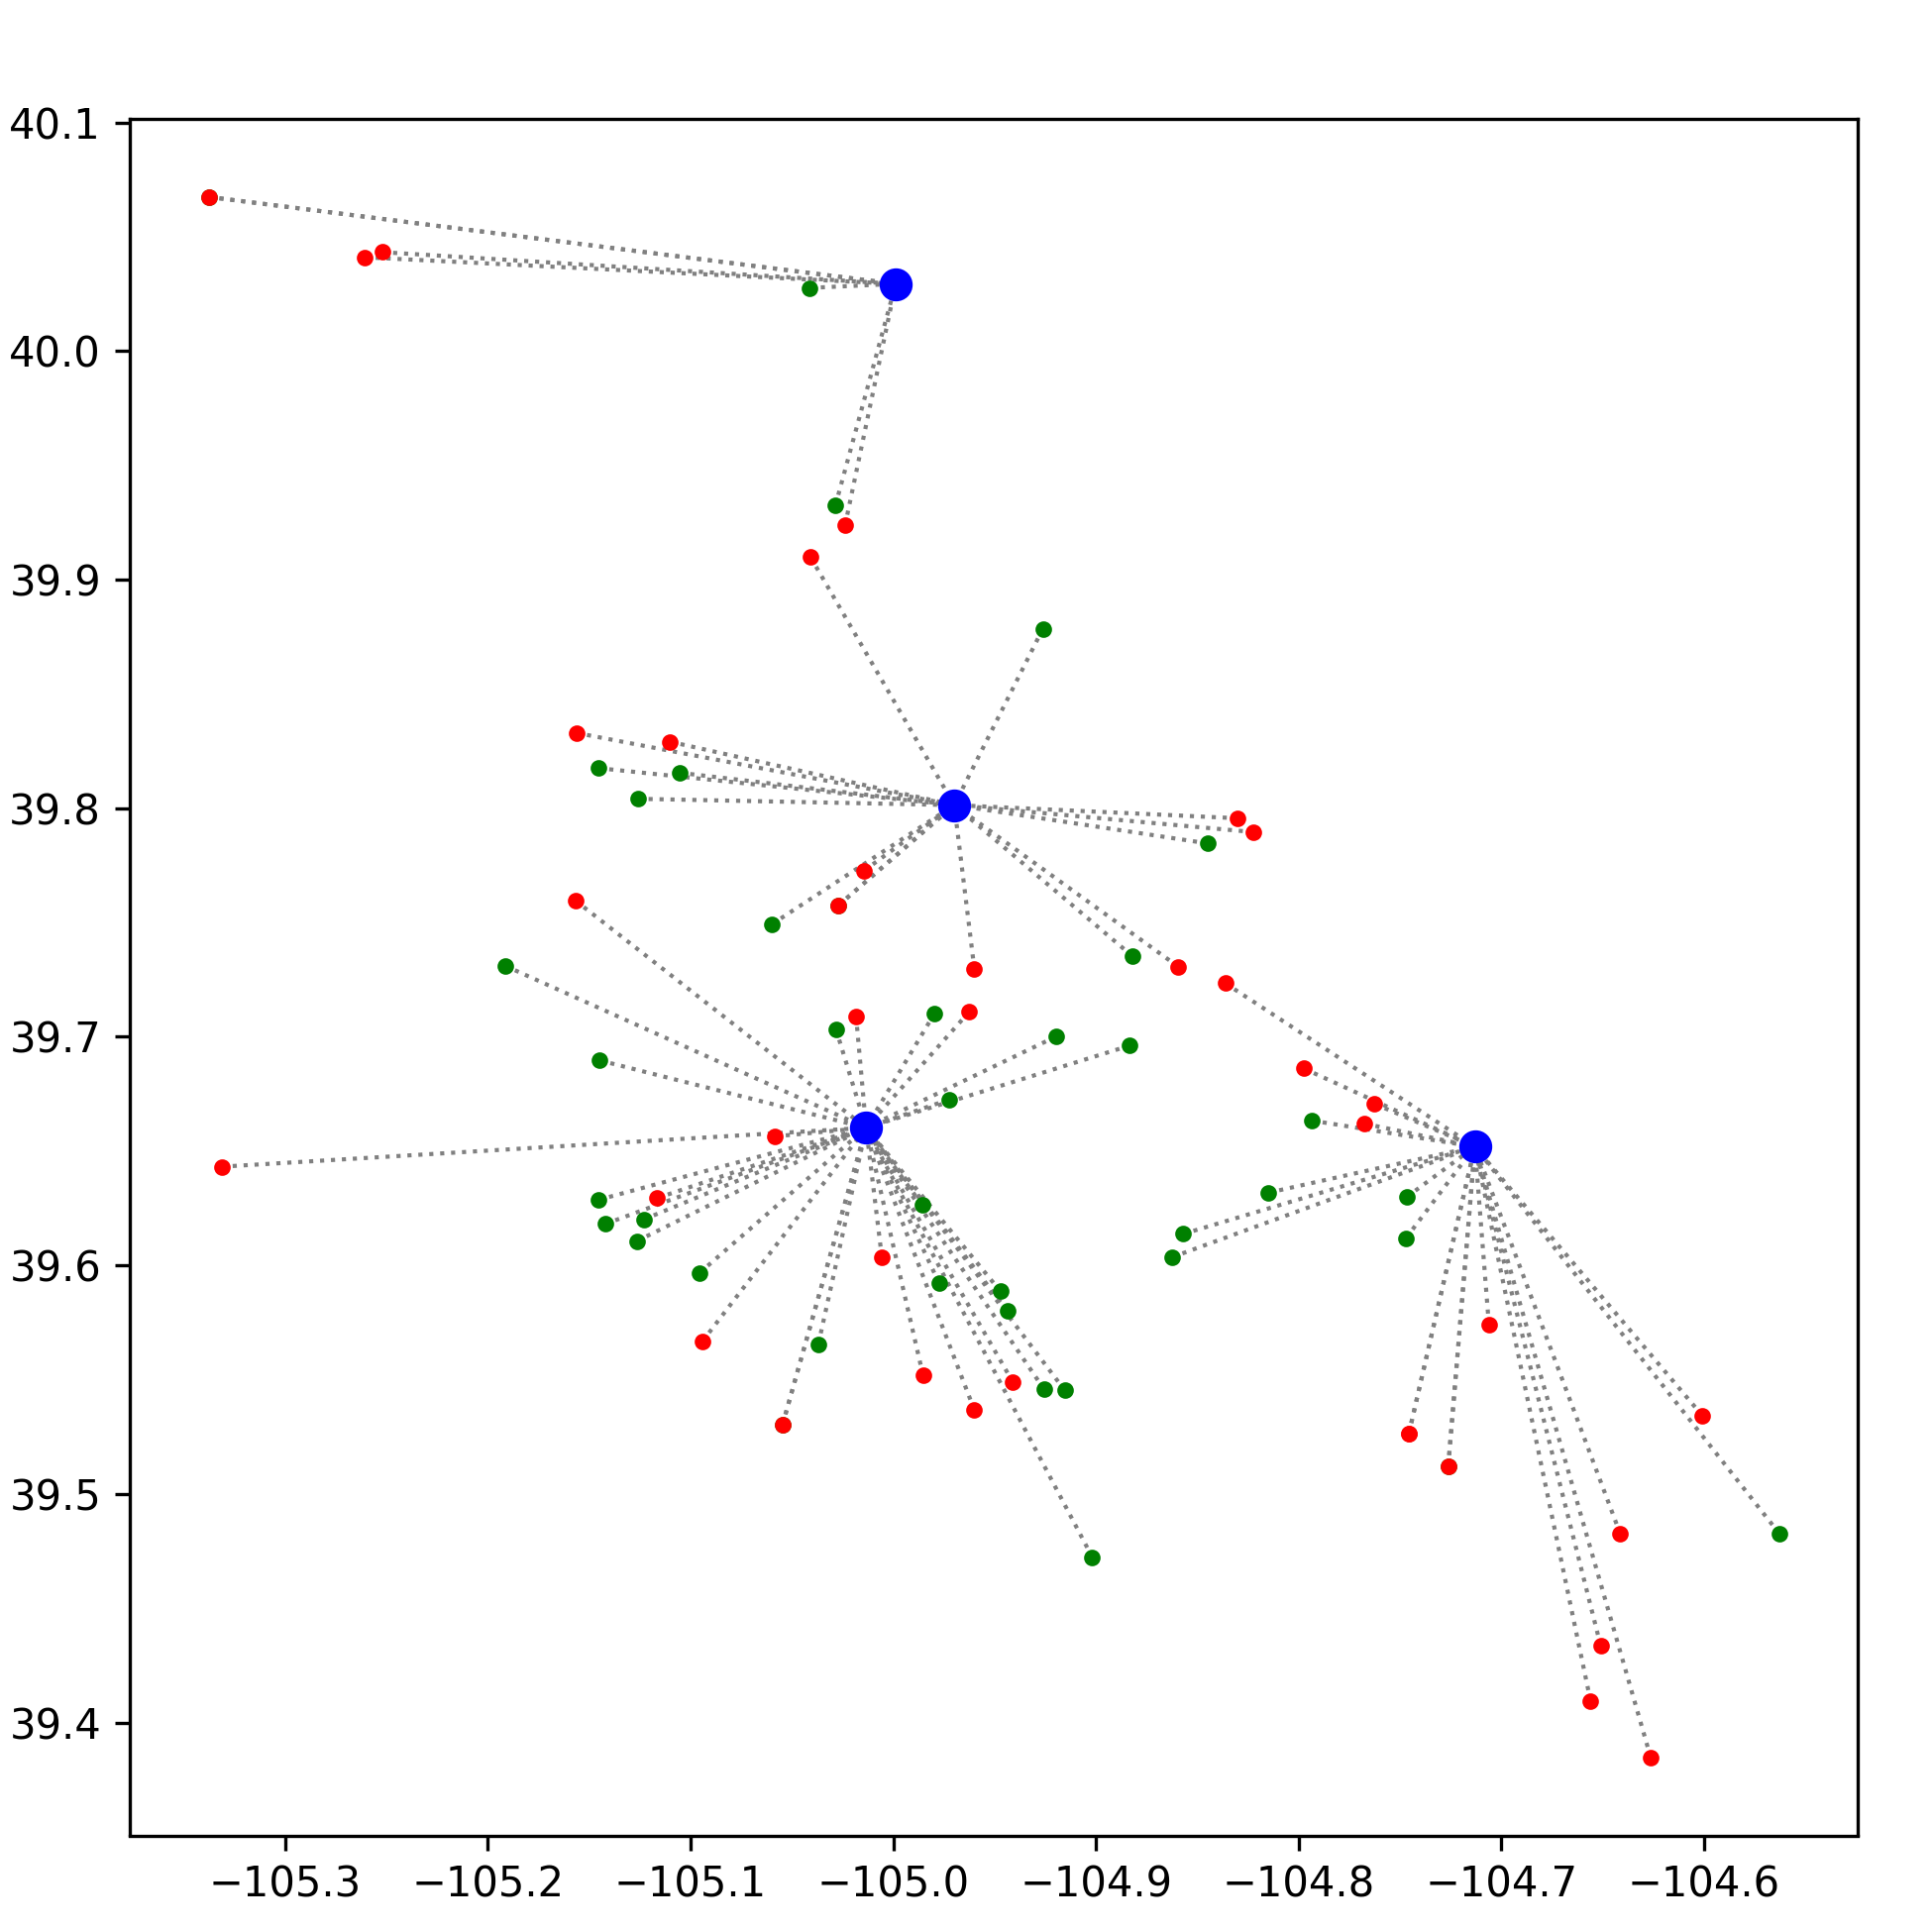
\includegraphics[width=7cm]{stars.png}\\
	With an empty truck, we can go do a pickup...
	\end{center}
\end{frame}

\section{Triangles}
\begin{frame}{A Small Example}
	\begin{center}
	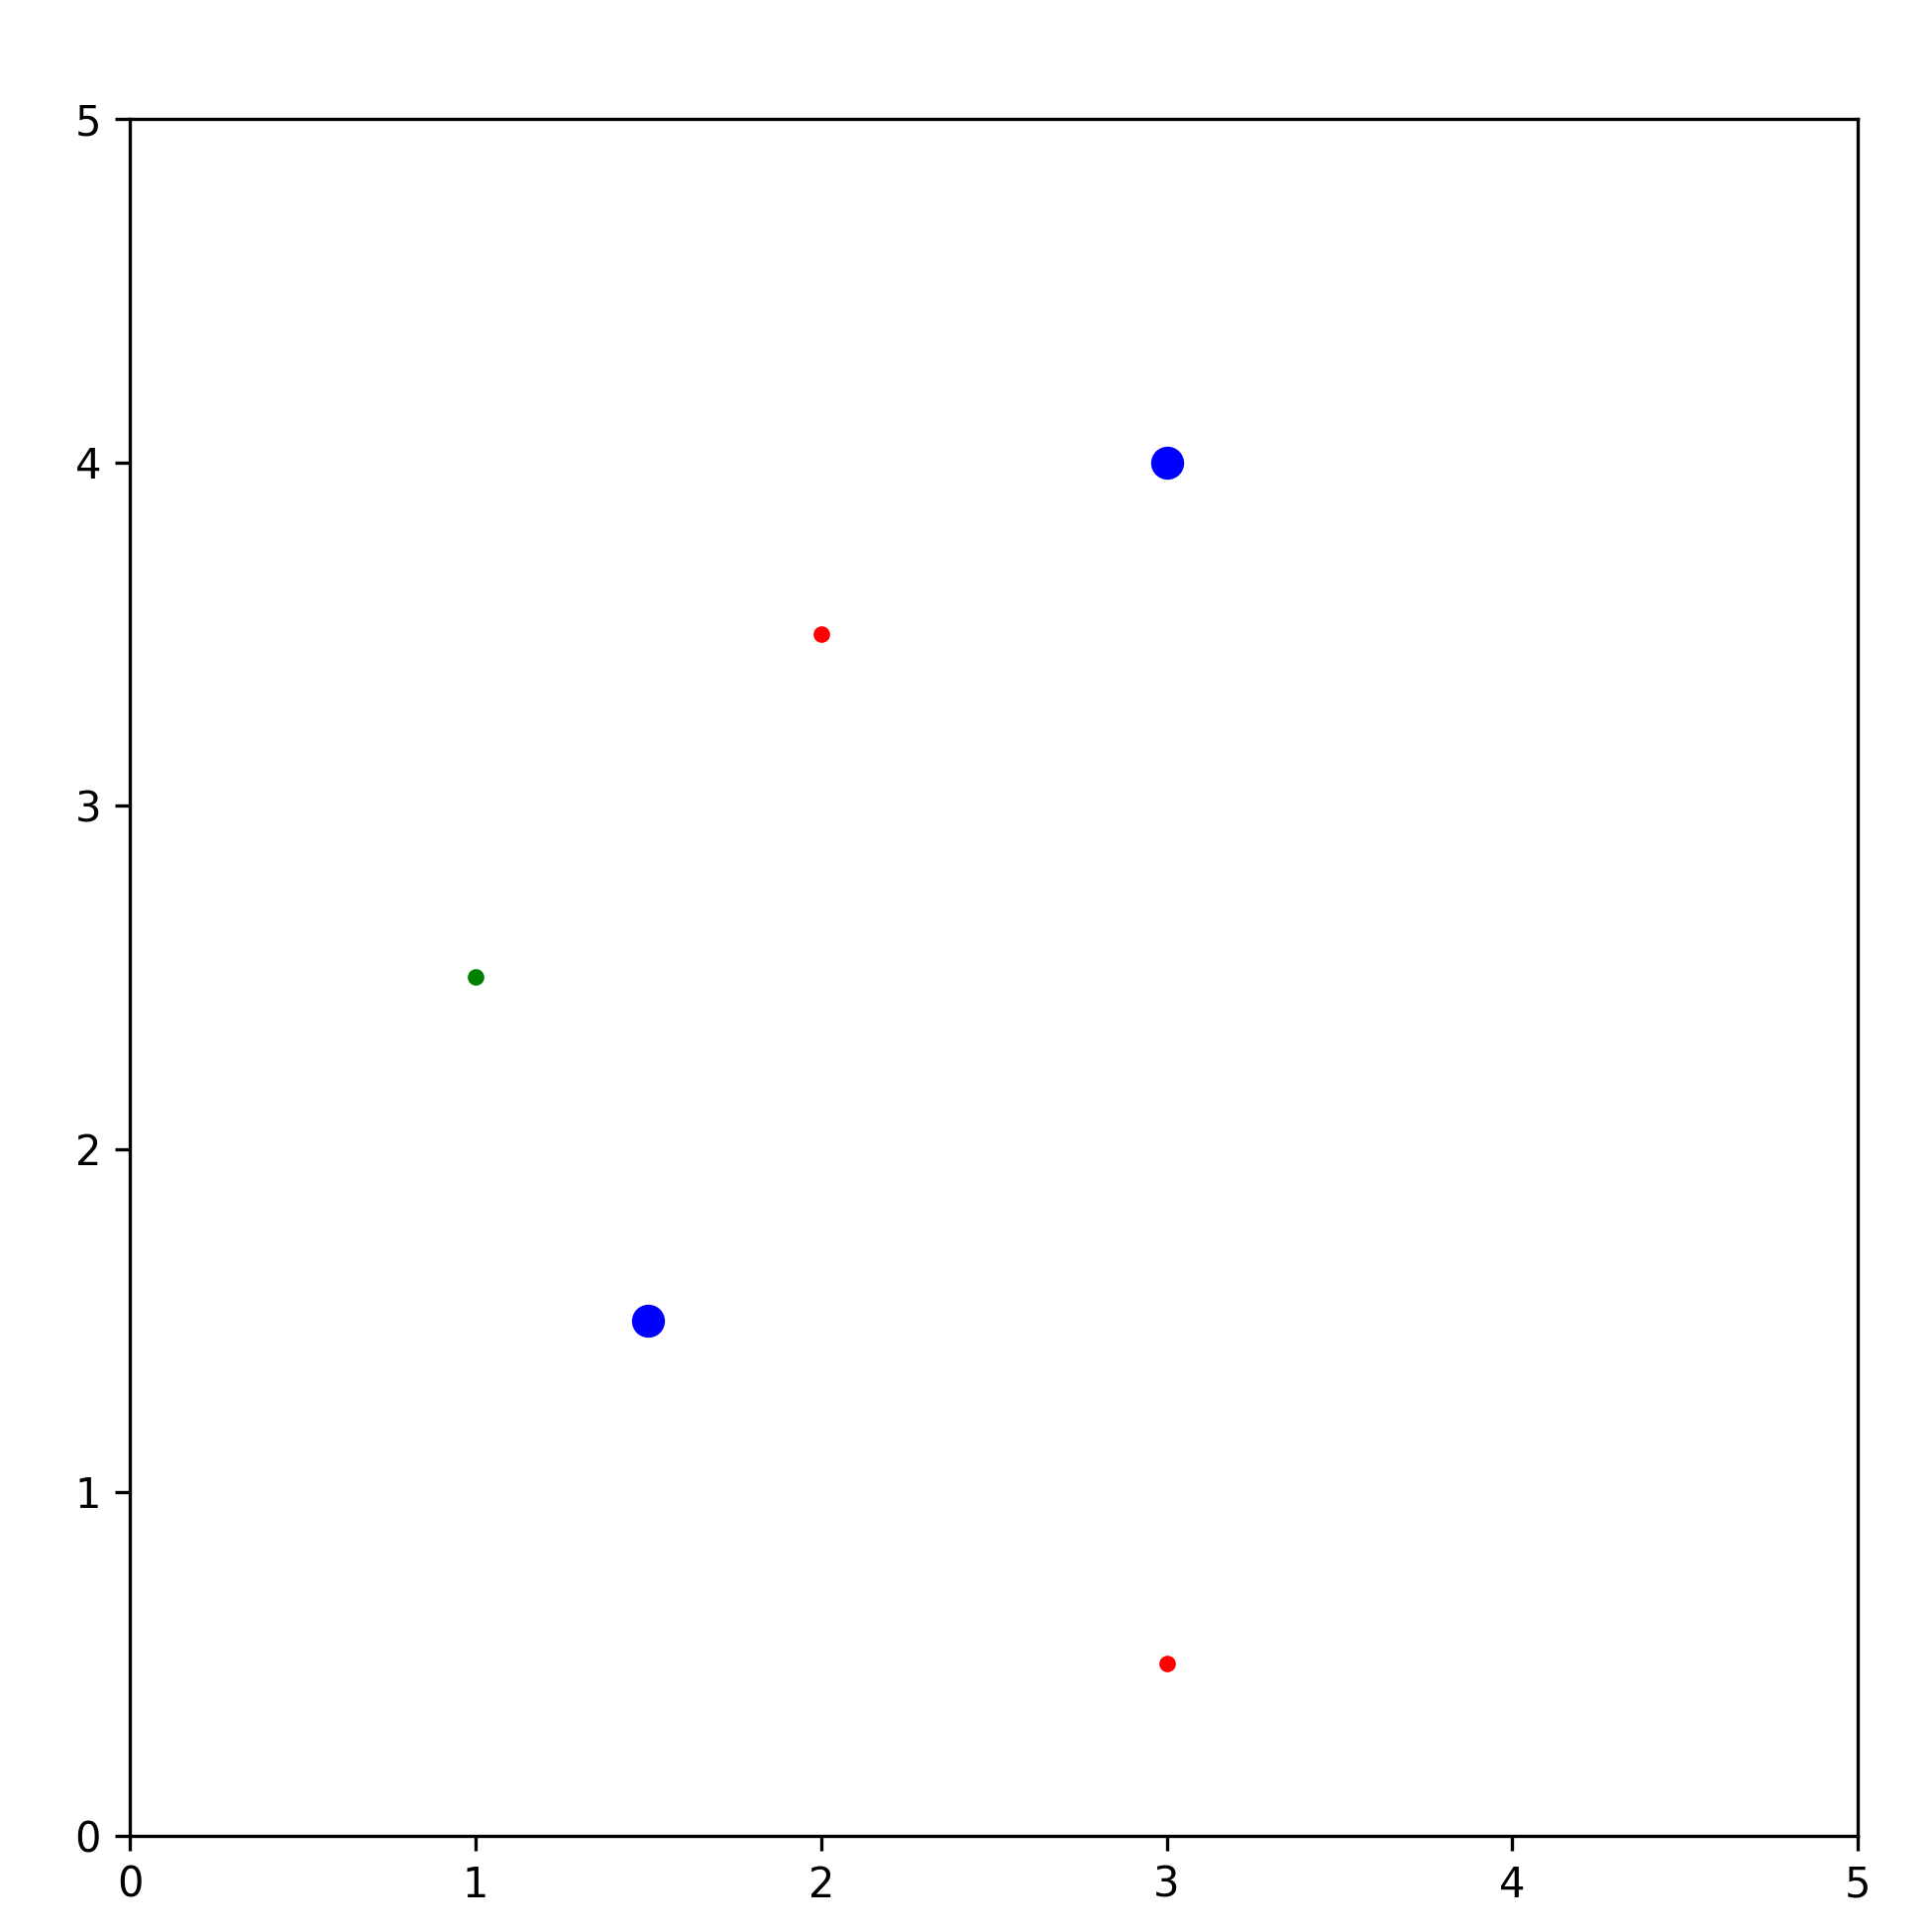
\includegraphics[width=7cm]{small_ex_empty.png}\\
	Nothing too complicated...
	\end{center}
\end{frame}

\begin{frame}{A Small Example}
	\begin{center}
	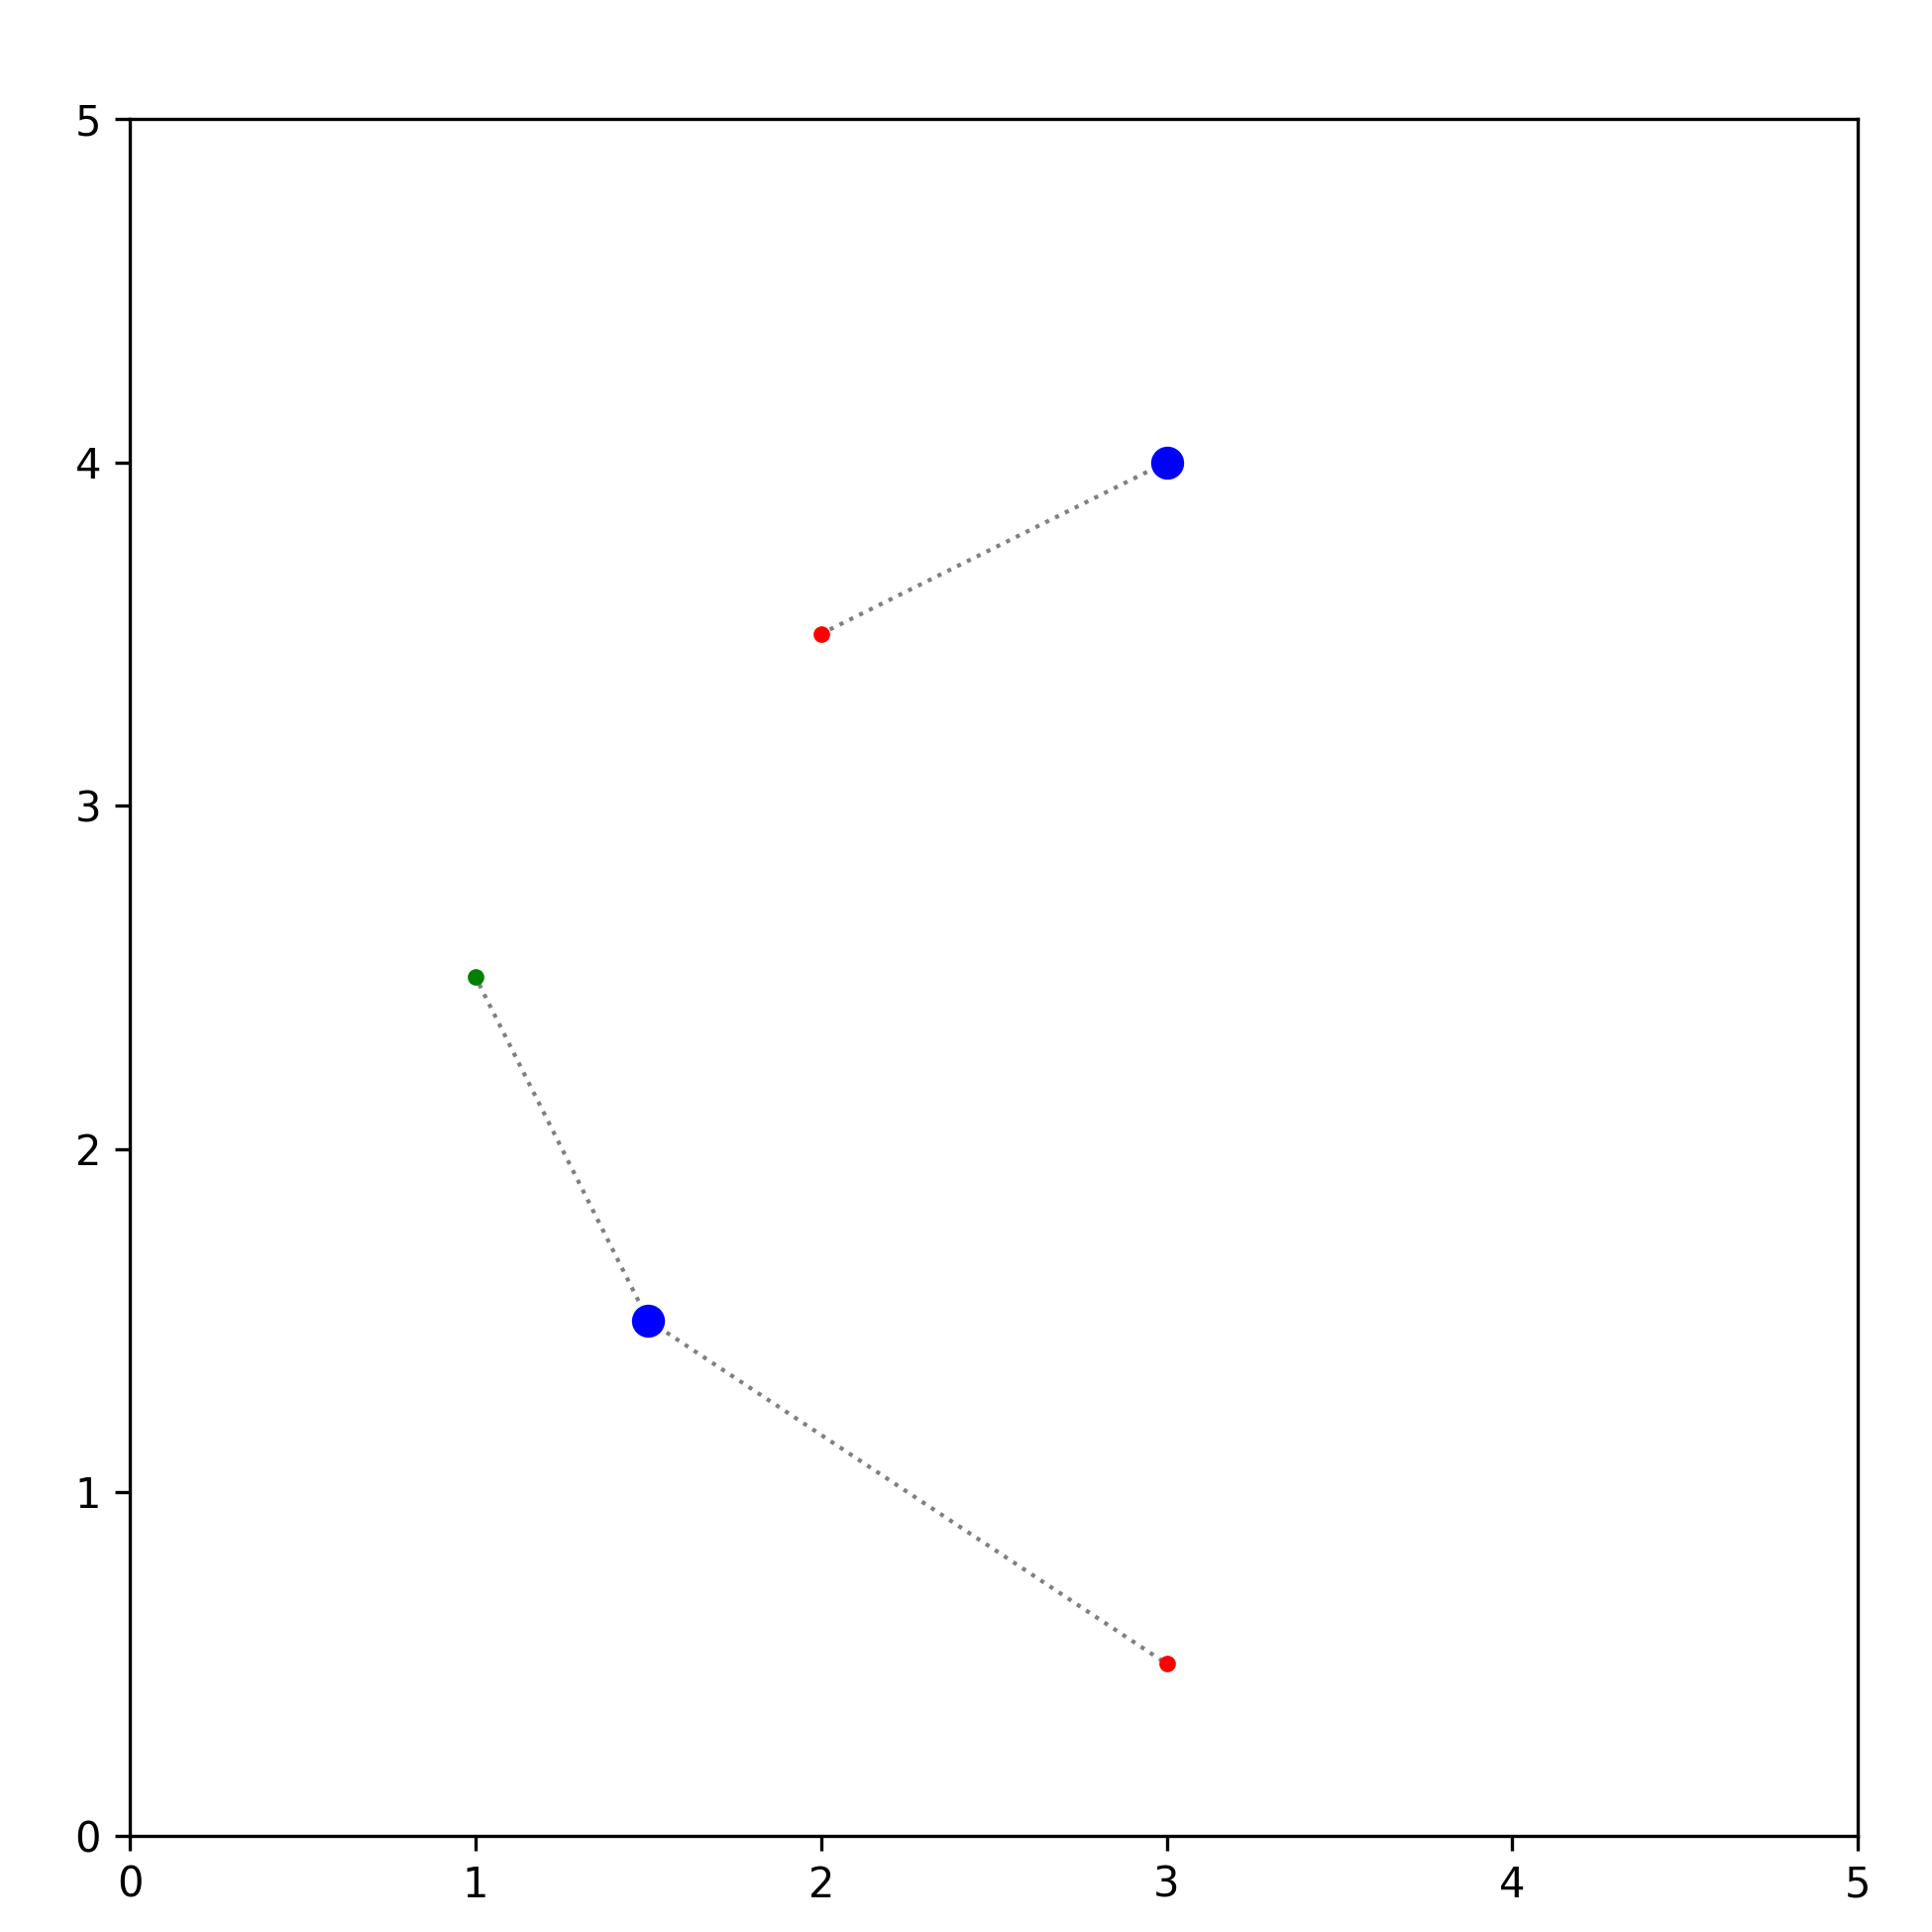
\includegraphics[width=7cm]{small_ex_star.png}\\
	Stars
	\end{center}
\end{frame}

\begin{frame}{A Small Example}
	\begin{center}
	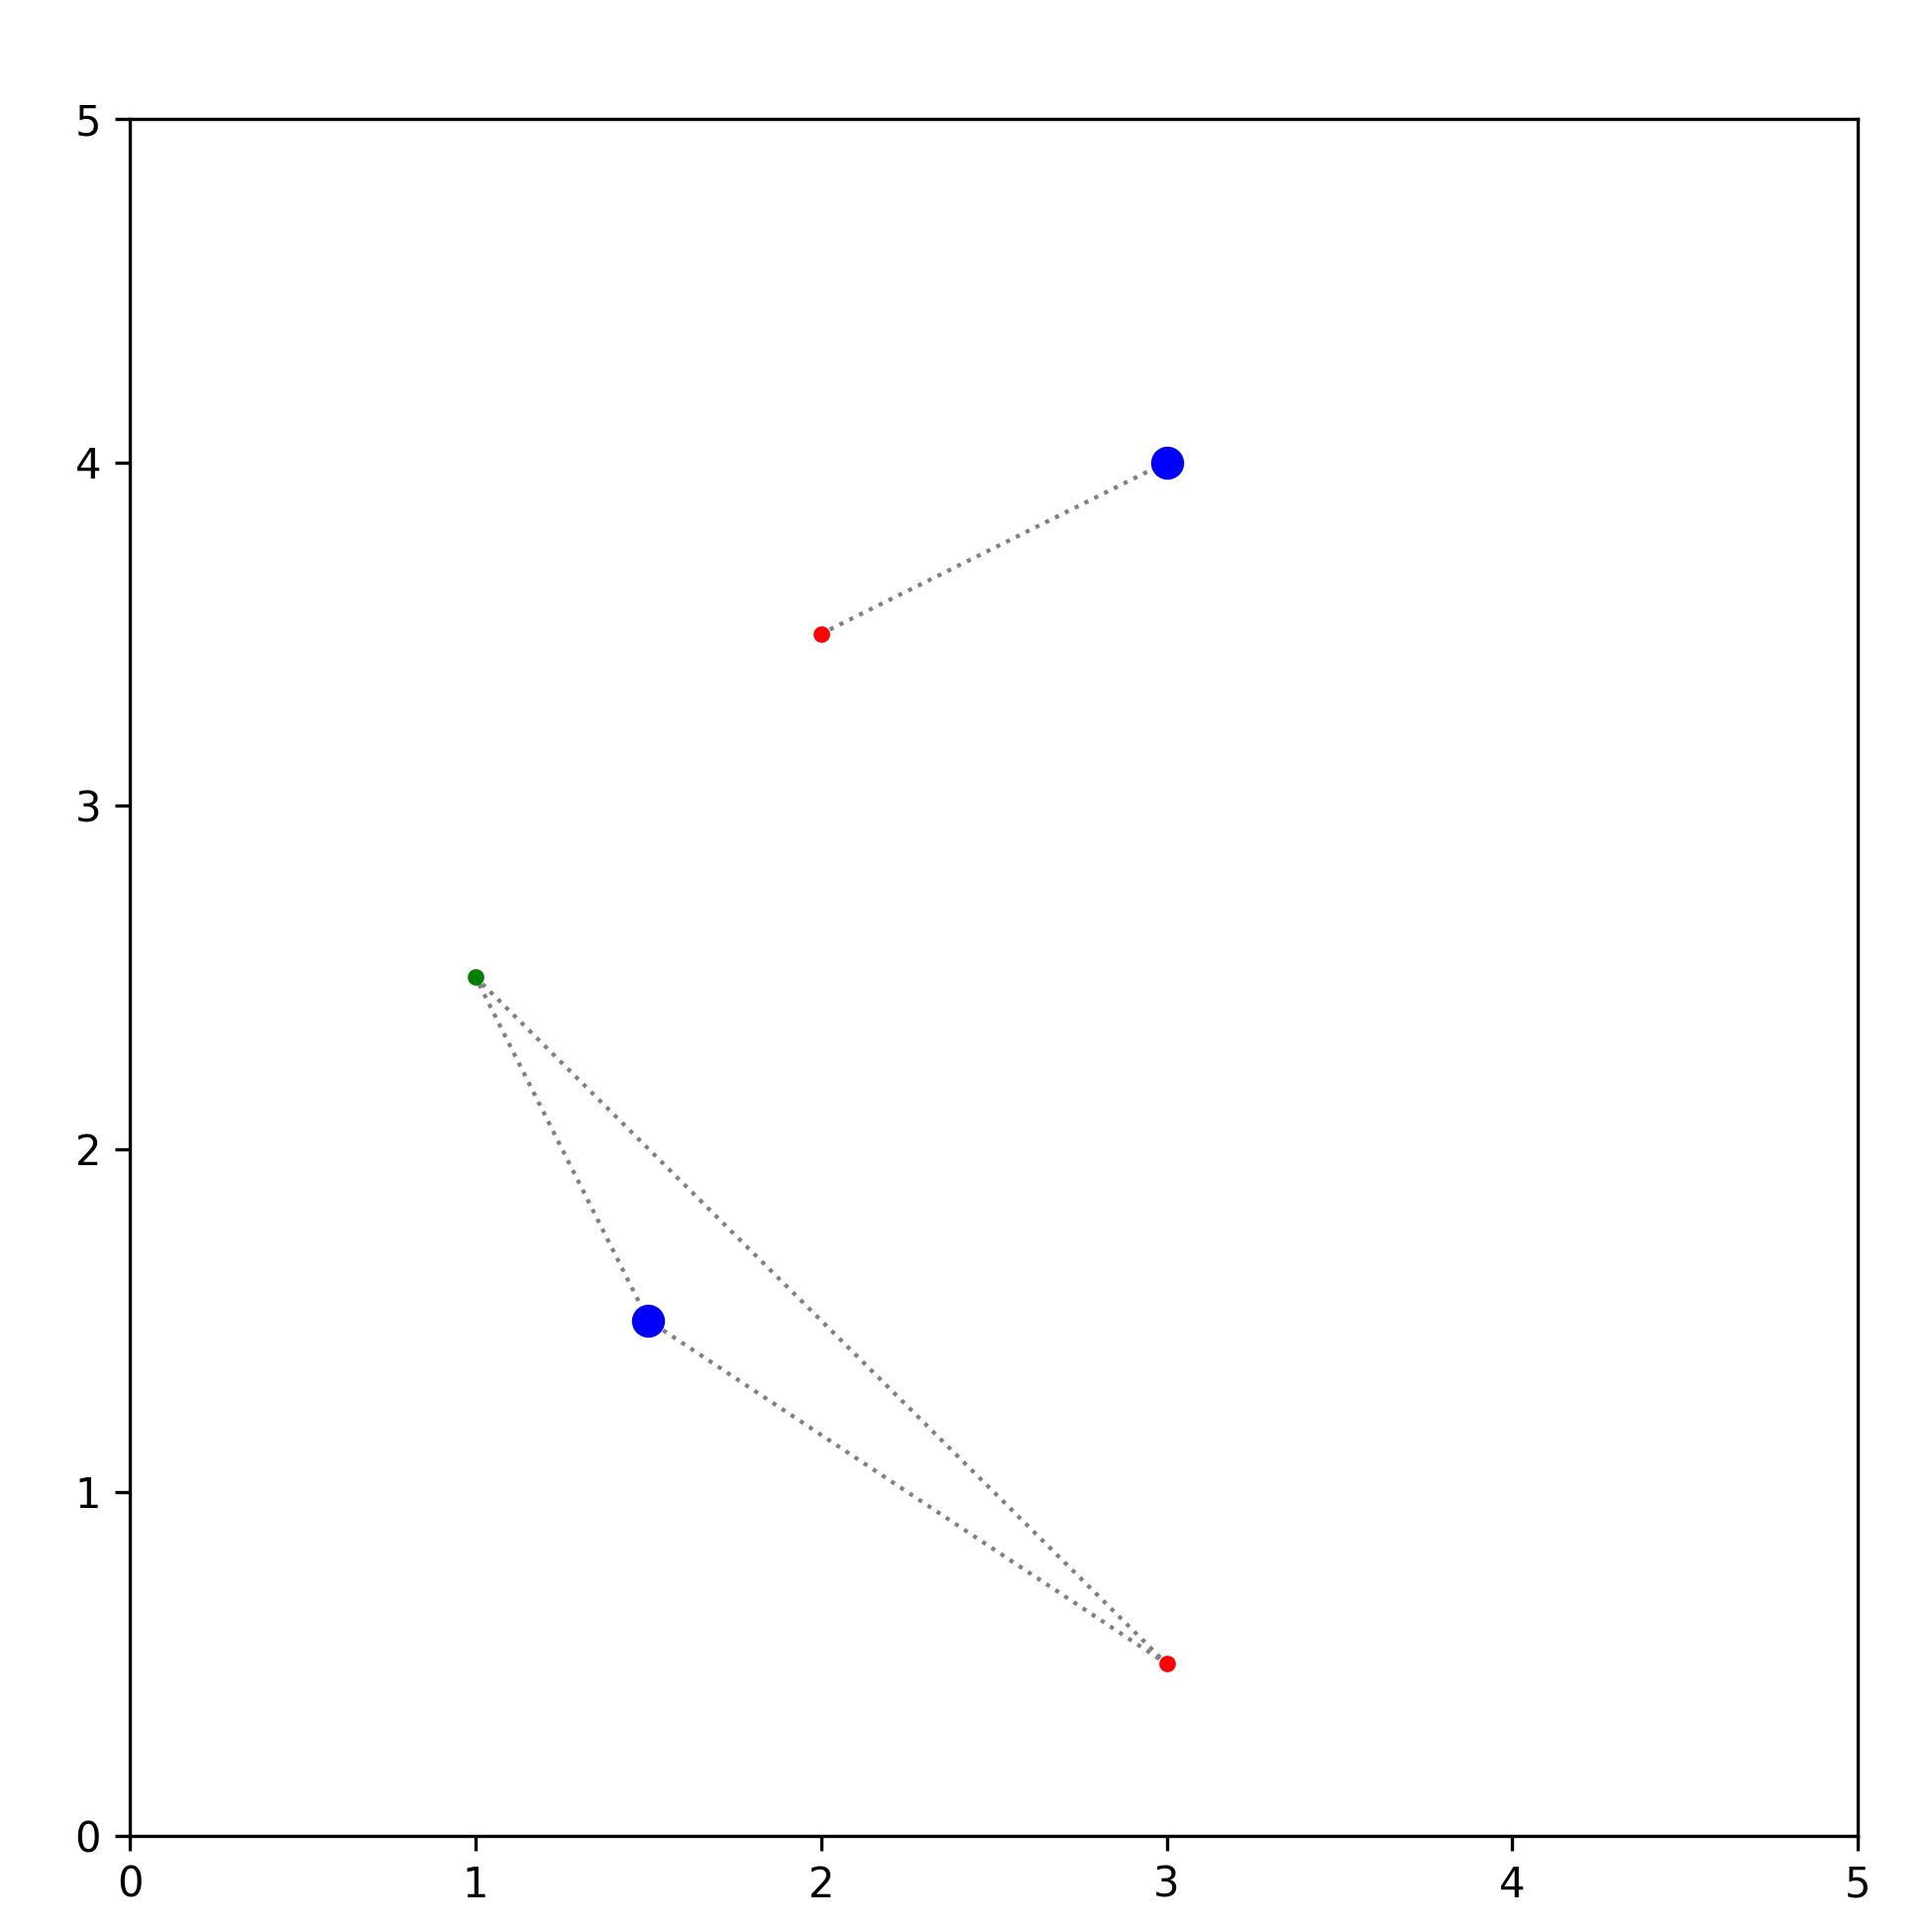
\includegraphics[width=7cm]{small_ex_ok.png}\\
	A triangle
	\end{center}
\end{frame}

\begin{frame}{A Small Example}
	\begin{center}
	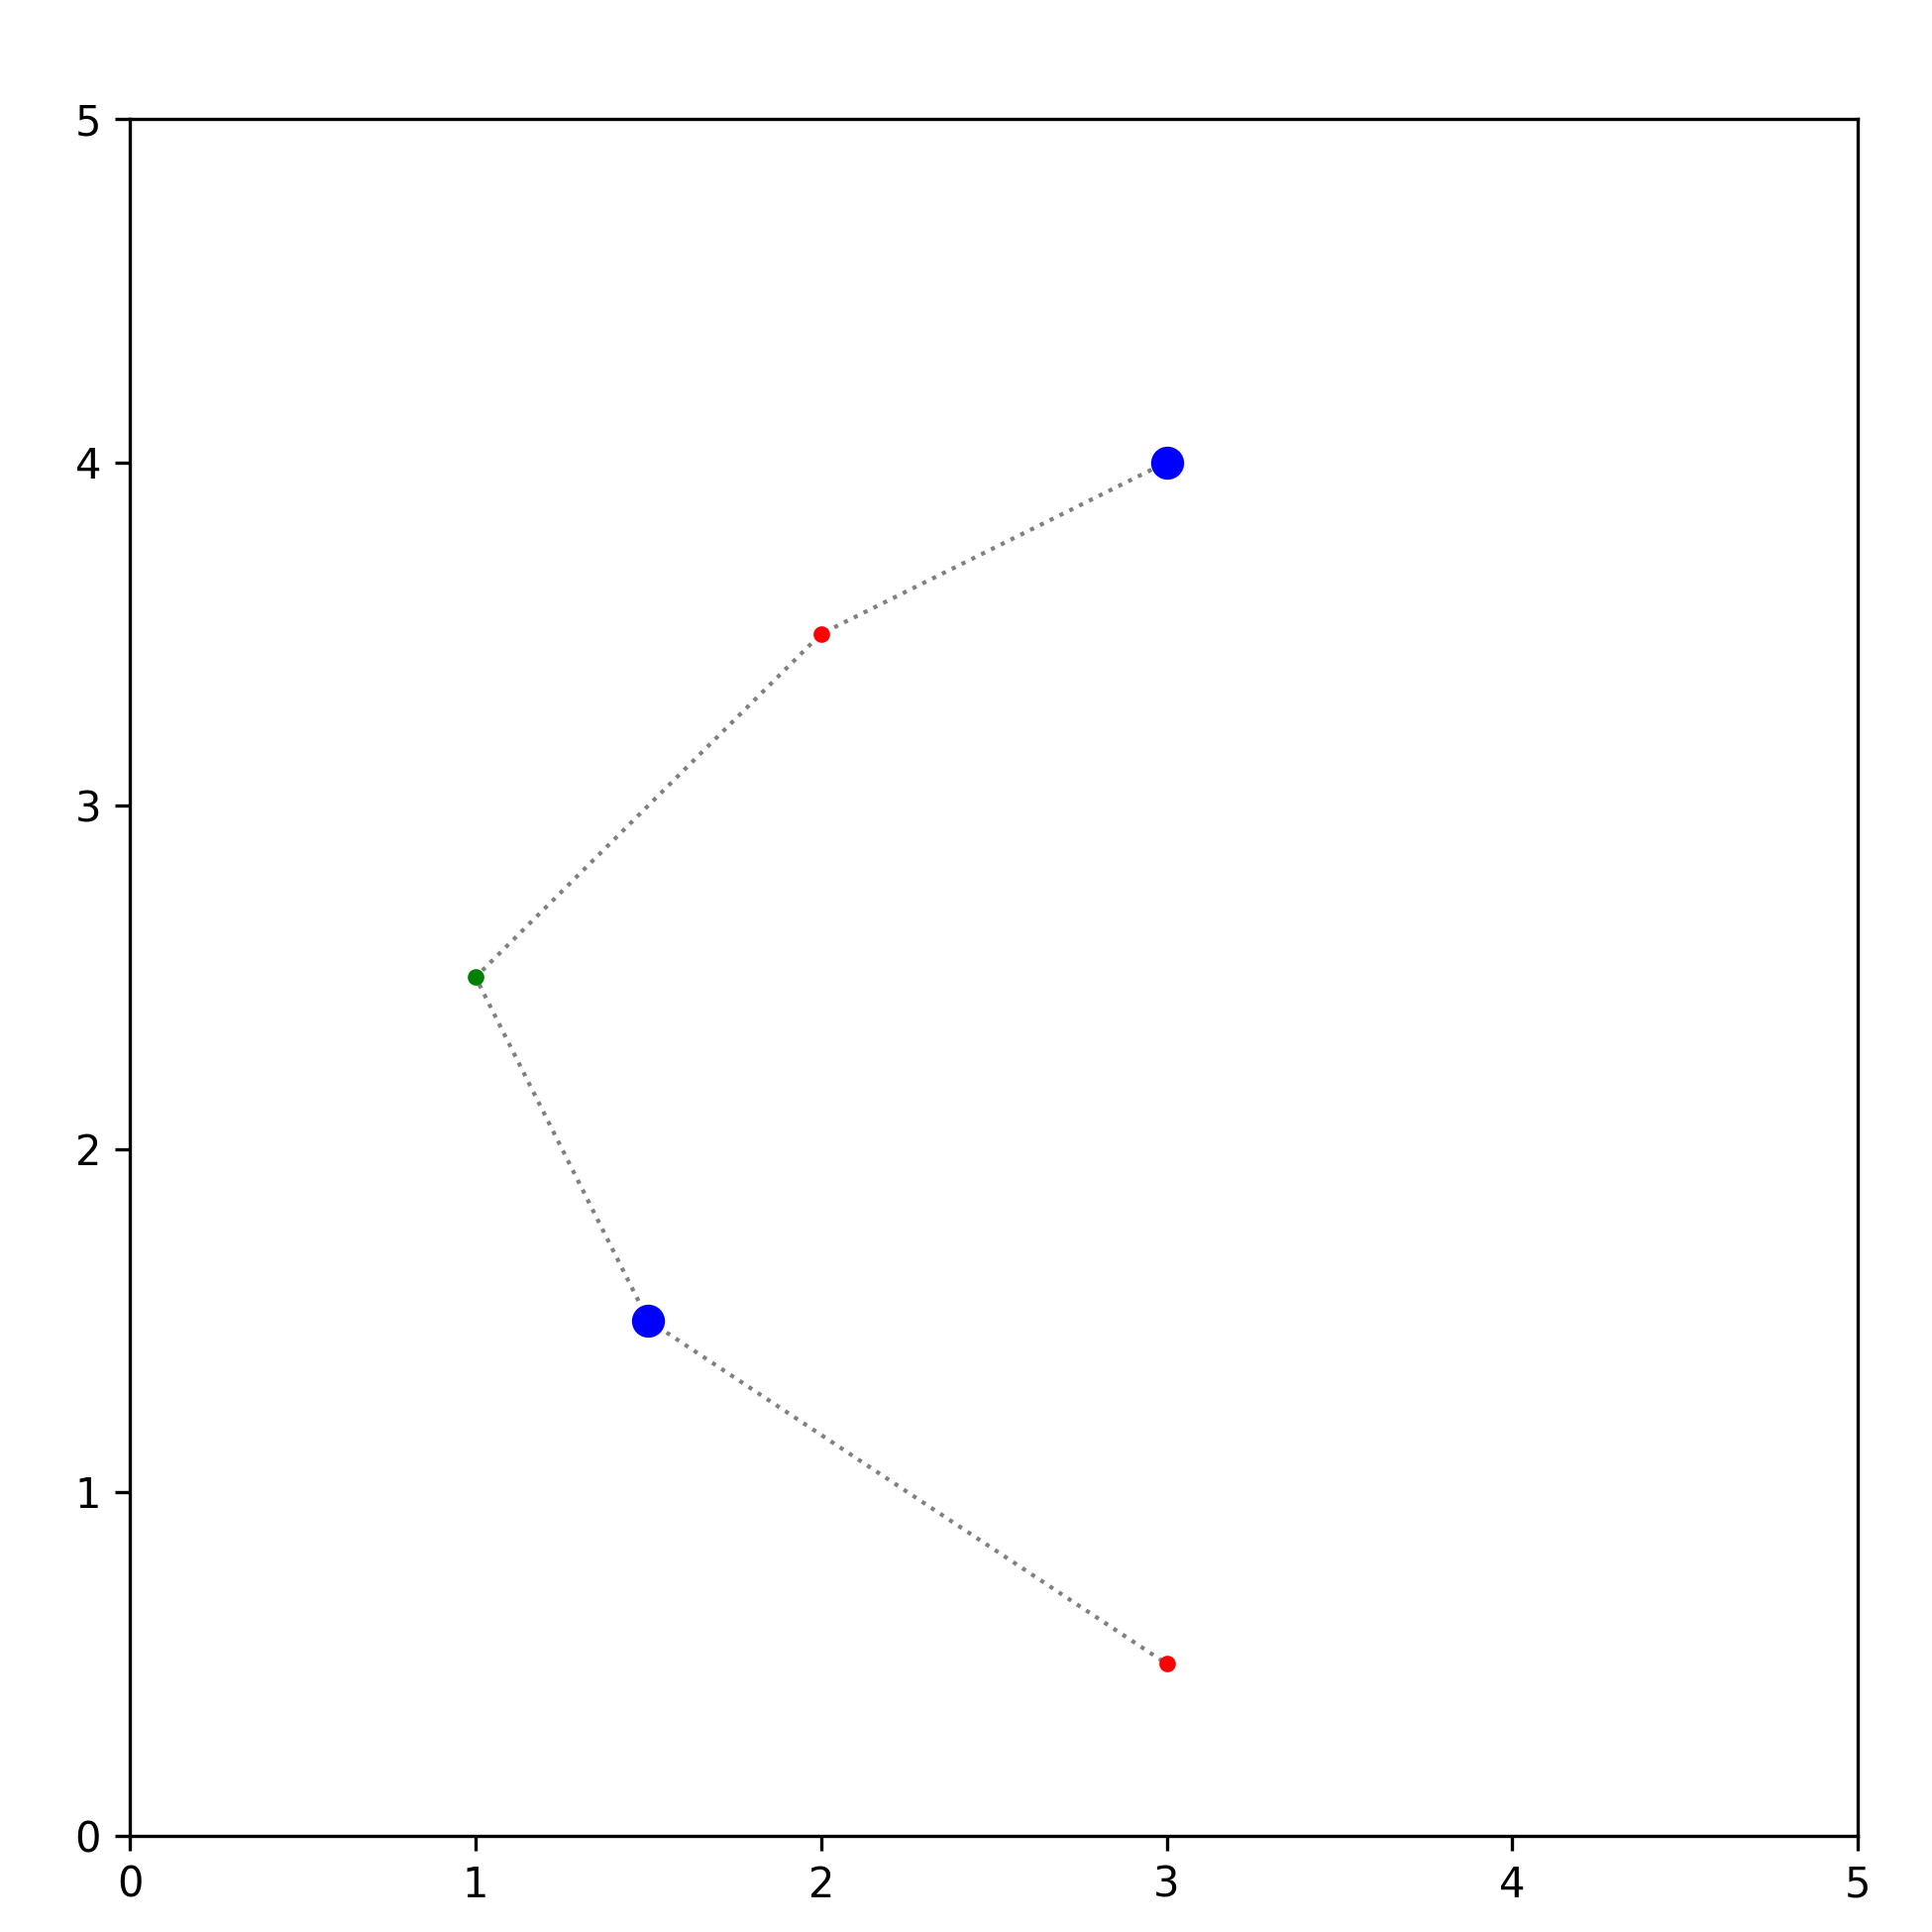
\includegraphics[width=7cm]{small_ex_best.png}\\
	A better ``triangle"
	\end{center}
\end{frame}

\begin{frame}{A Question}
	\begin{center}
		How do we find the best triangles?
	\end{center}
	It turns out this problem has been studied before, between two sets (here, deliveries and pickups), what is the least ``cost" way to match them up?
	
	\begin{center}
	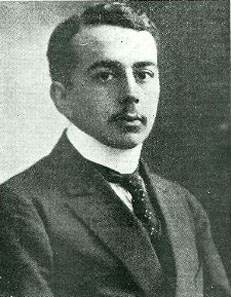
\includegraphics[height=3cm]{konig.jpg}\qquad
	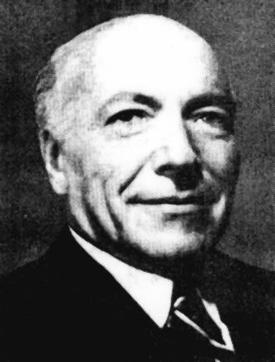
\includegraphics[height=3cm]{egervary.jpg}\\
	K\H onig and Egerv\'ary
	\end{center}

	In this context, ``cost'' means driving time.
\end{frame}

\begin{frame}{The Best Triangles}
	\begin{center}
	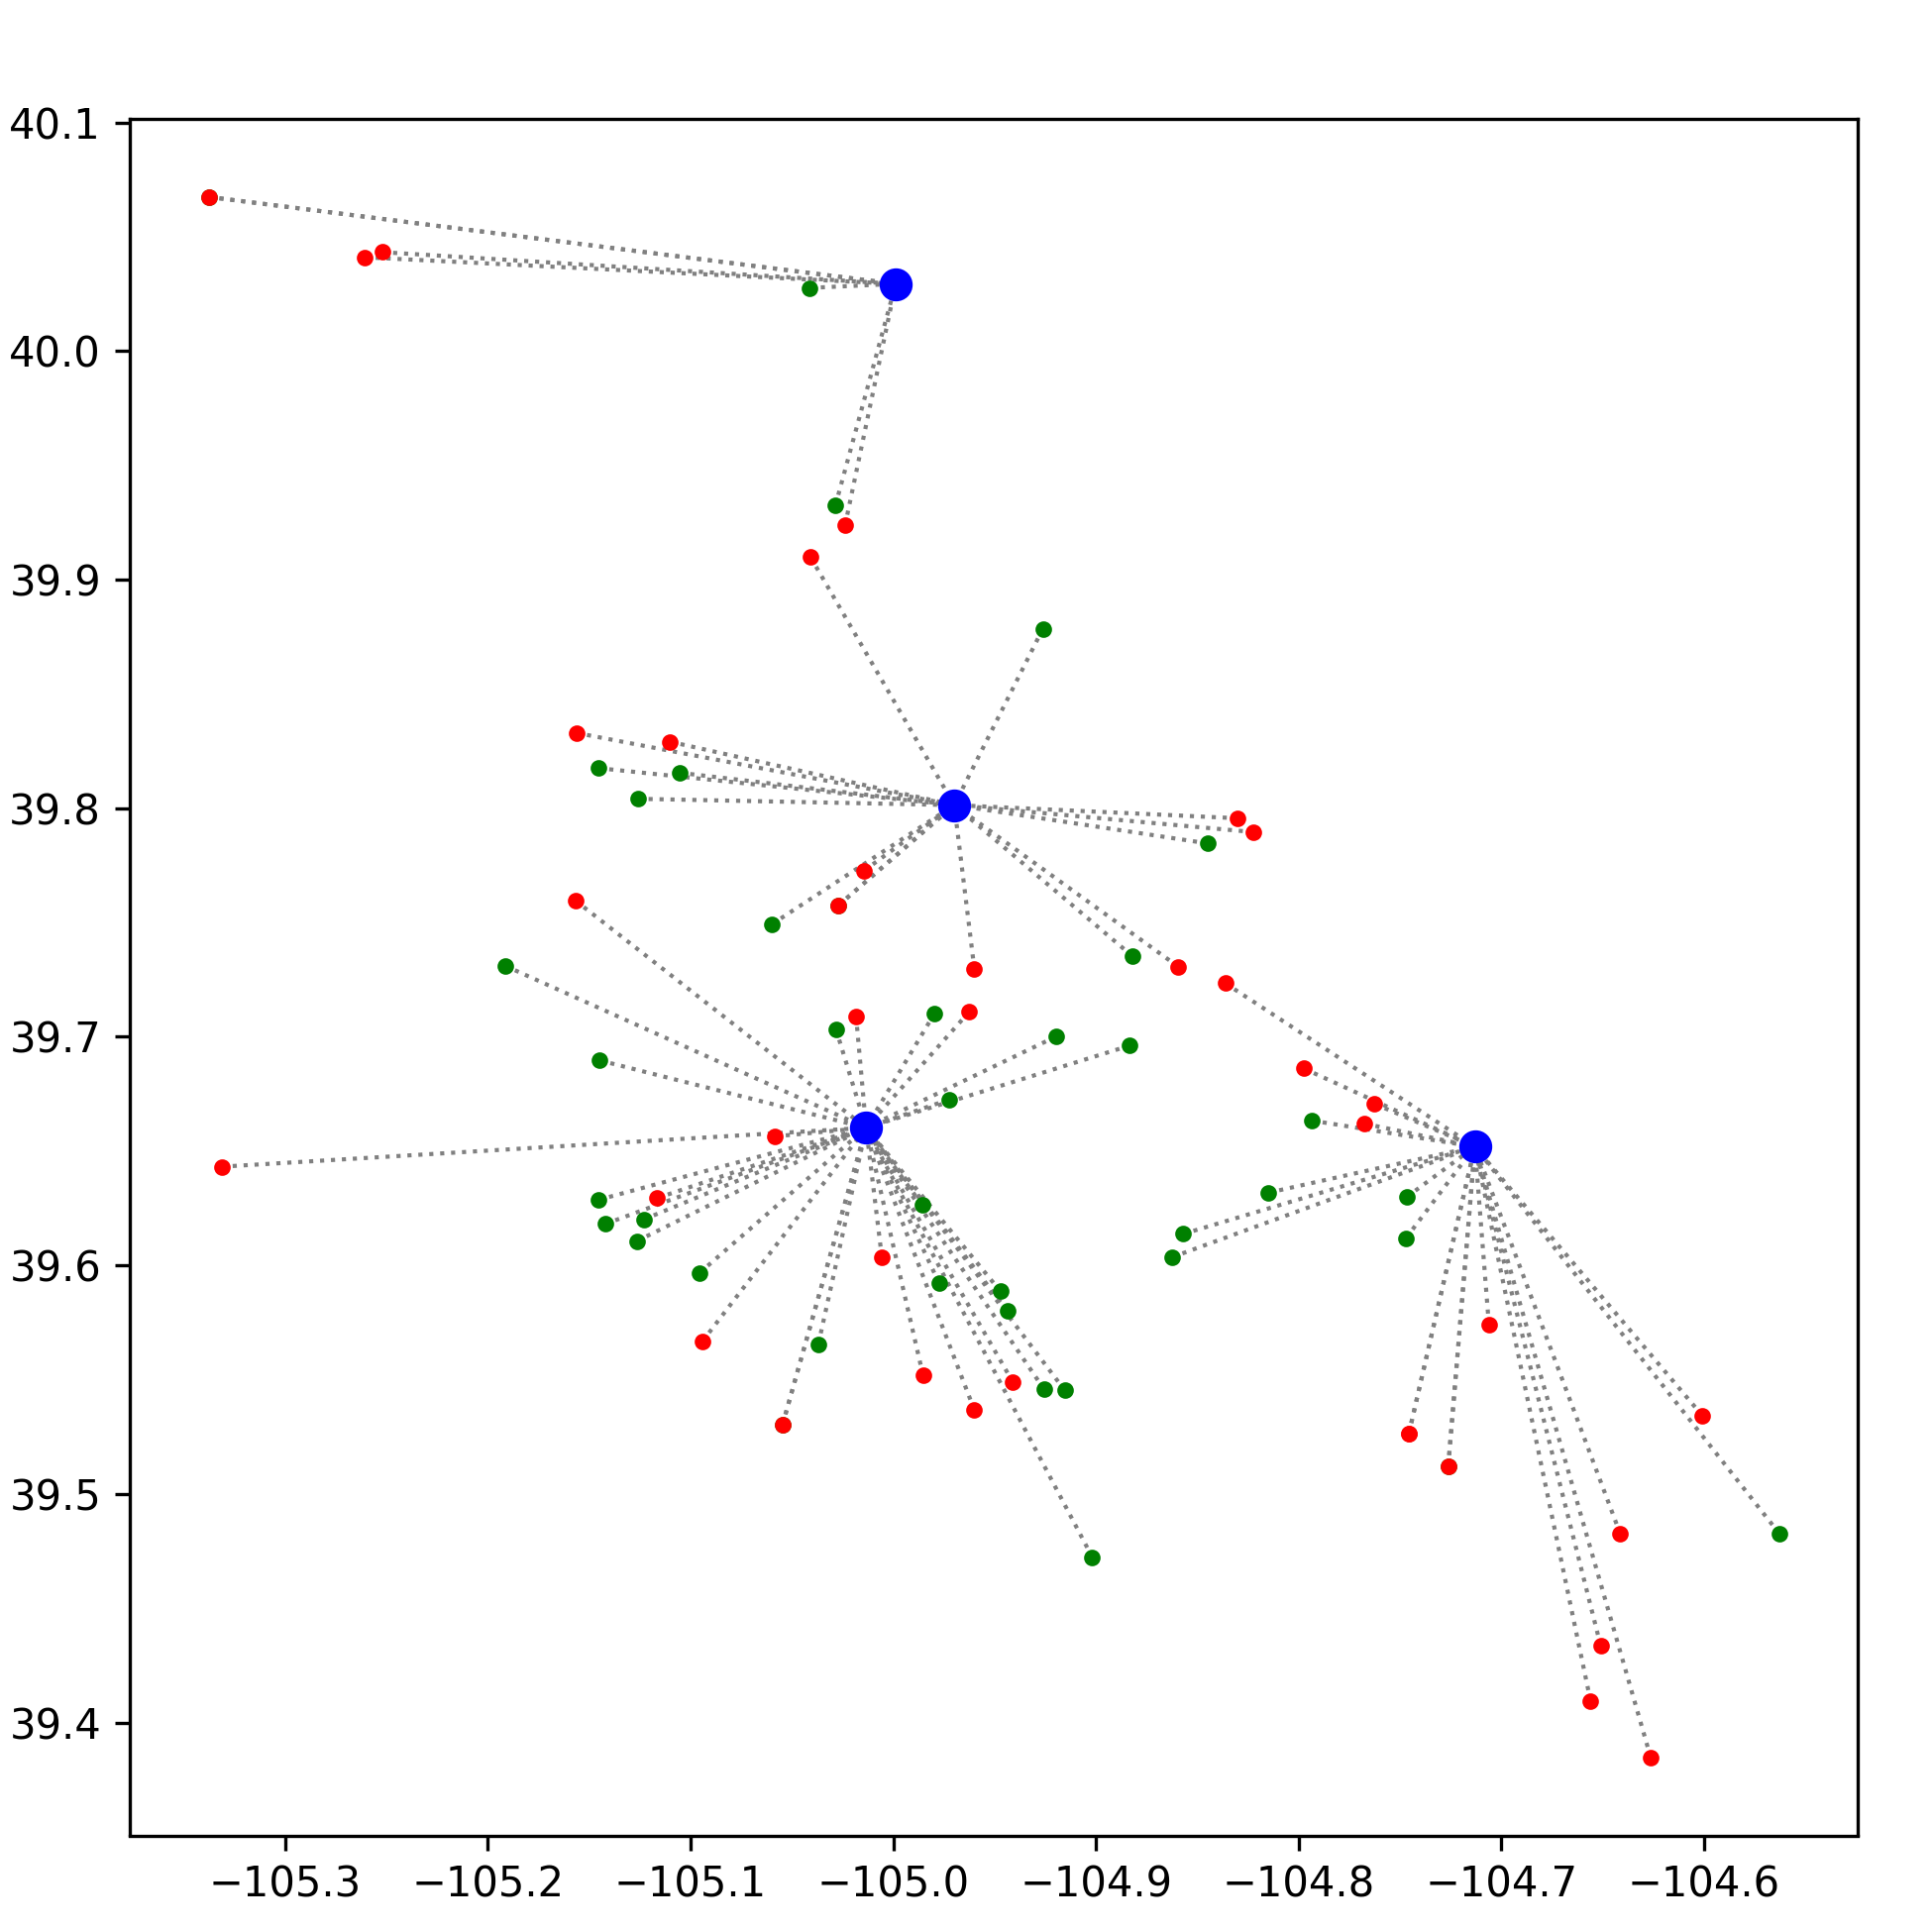
\includegraphics[width=7cm]{stars.png}\\
	What do they look like here?
	\end{center}
\end{frame}

\begin{frame}{The Best Triangles}
	\begin{center}
	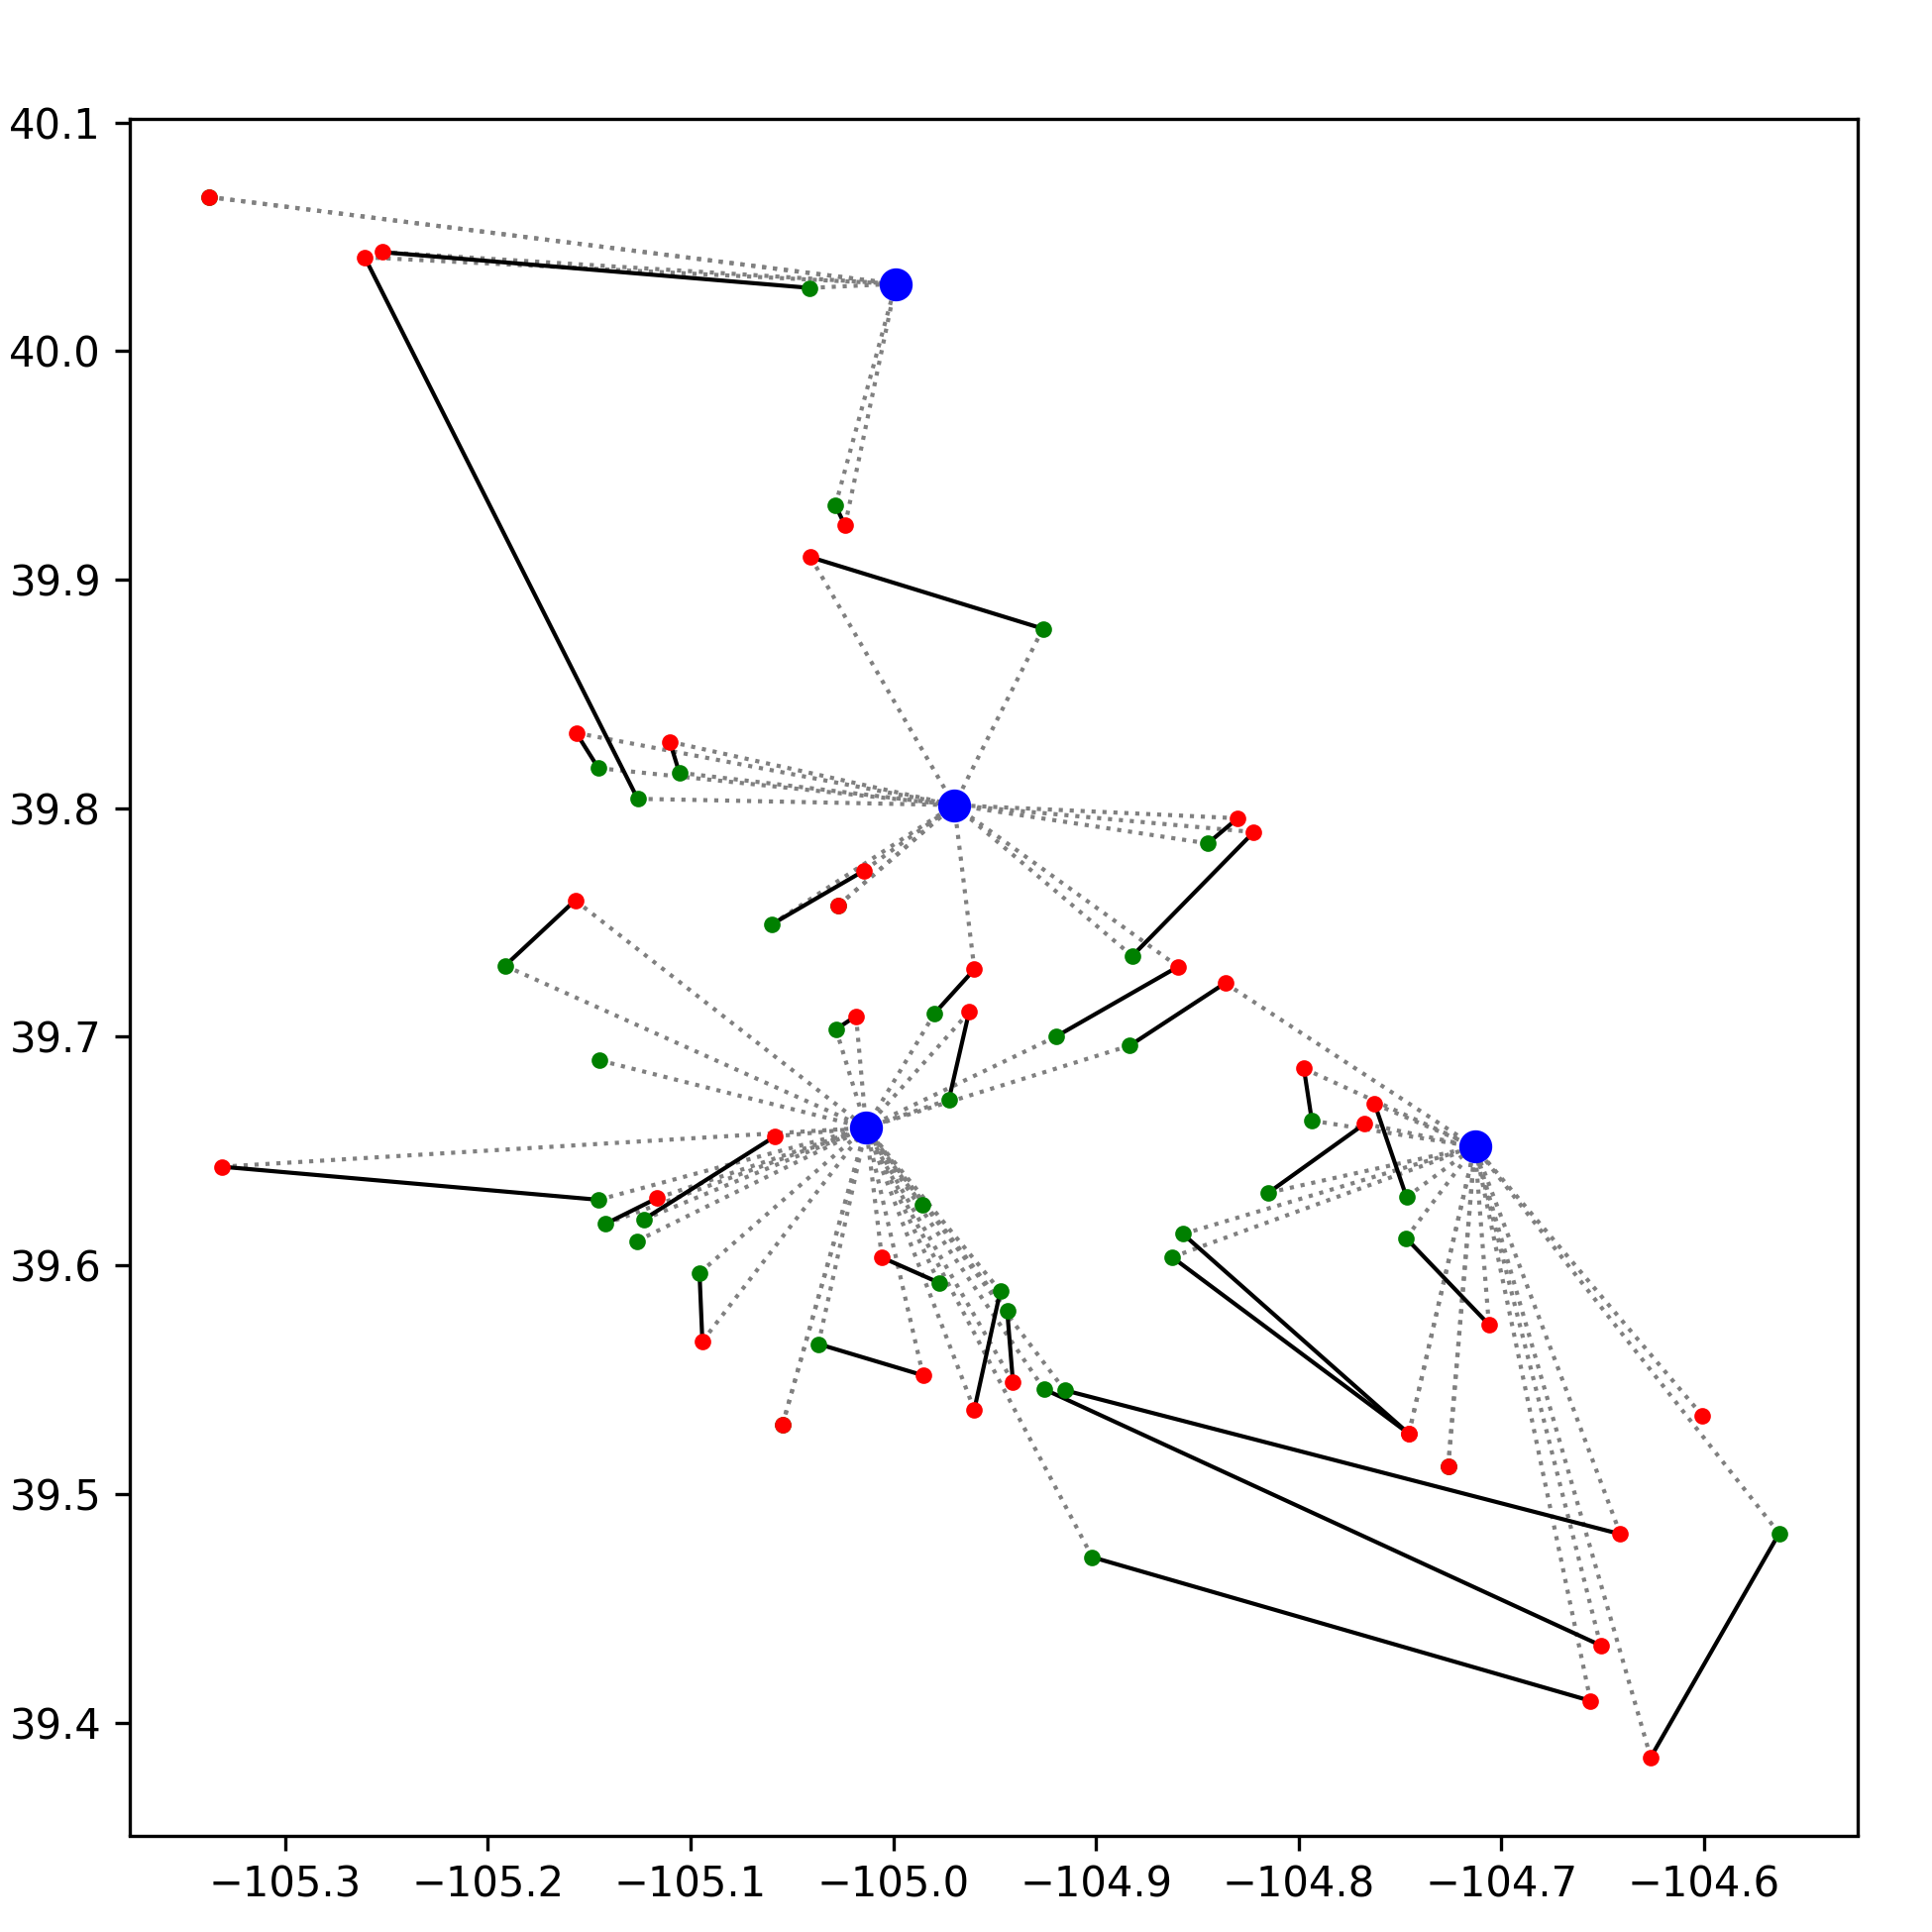
\includegraphics[width=7cm]{triangles.png}\\
	Tada!
	\end{center}
\end{frame}

\section{Transitions}
\begin{frame}{Moving Between Stars}
	\begin{center}
	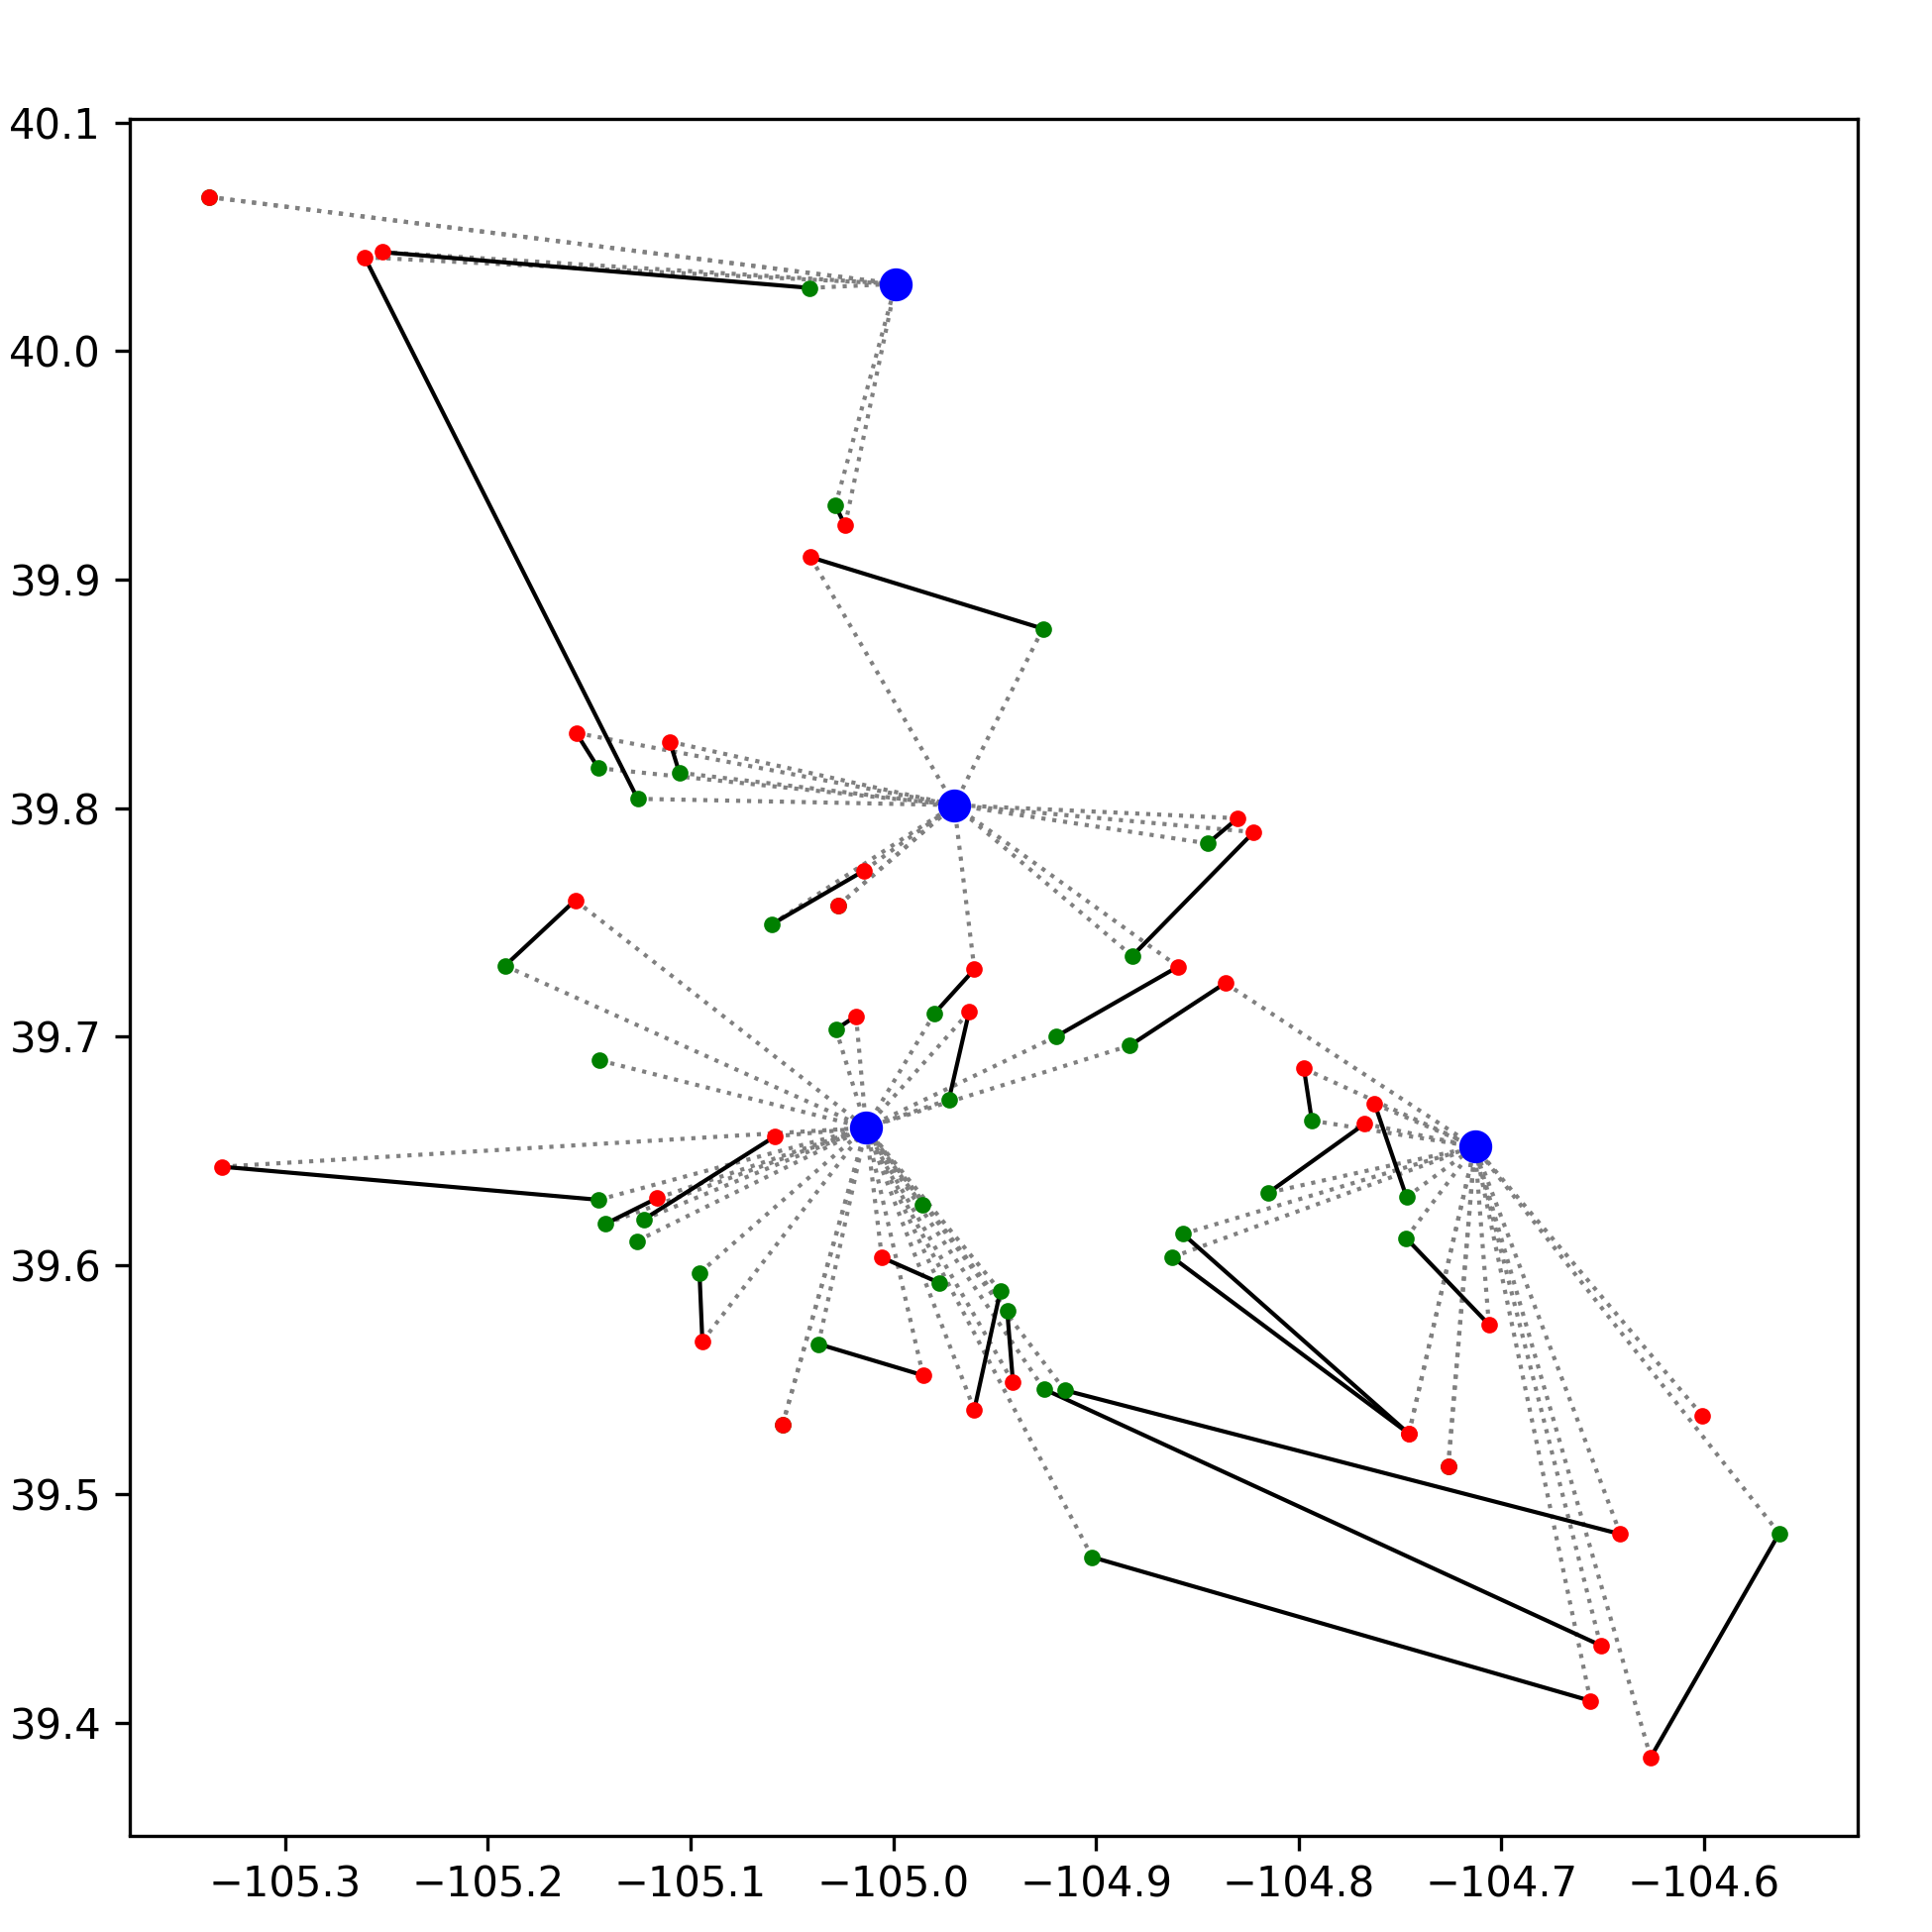
\includegraphics[width=7cm]{triangles.png}\\
	To go from one star to another, a choice must be made.
	\end{center}
\end{frame}

\section{Can Inventory Management}
\begin{frame}{A Balancing Act}
	Sometimes, the zone surrounding a storage yard may need more deliveries than the yard has cans.
	\begin{center}
		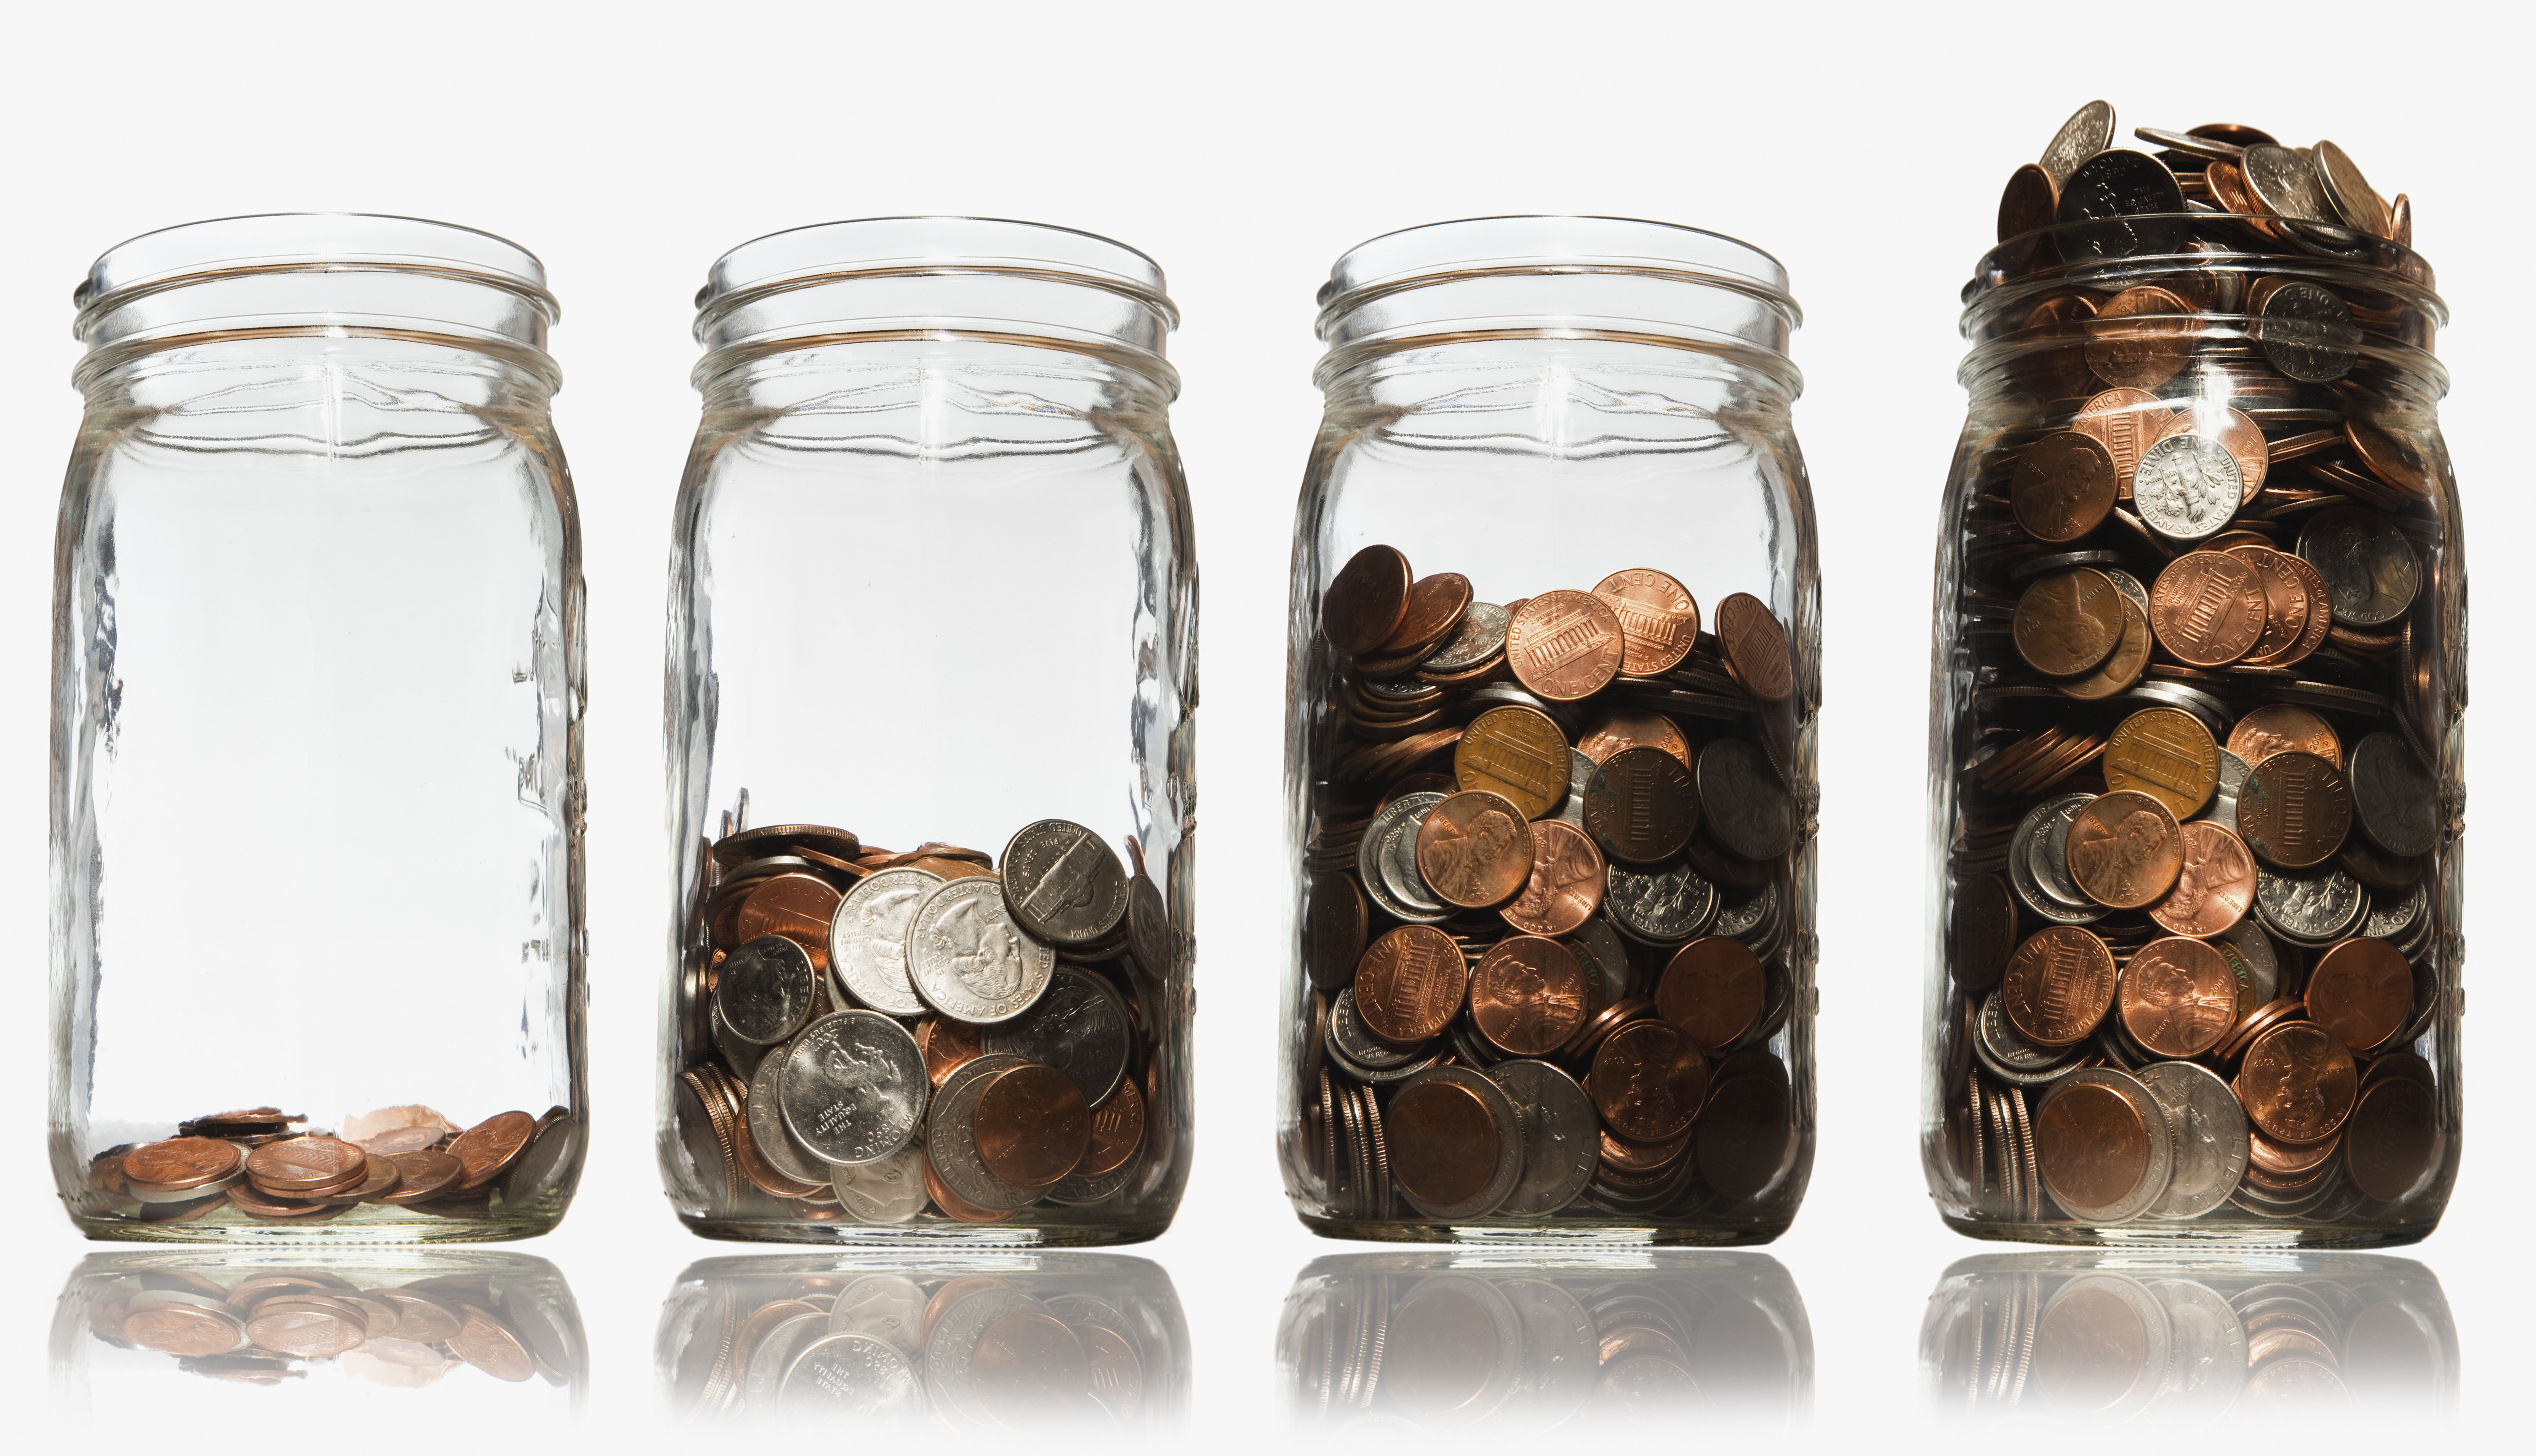
\includegraphics[width=7cm]{coins.jpg}
	\end{center}
	\pause
	In order to remedy this, we take into account can inventories while making transfers, and verify that we don't tell a driver to pick up a can from a yard which doesn't have any.
\end{frame}

\section{Route Building}
\begin{frame}{Where a Truck Must Go}
	Some trucks are special, they may be small enough to go where others can't, or big enough to carry heavy loads that others can't. The problem is, there aren't many of them.
	\vspace{.5cm}
	\begin{center}
		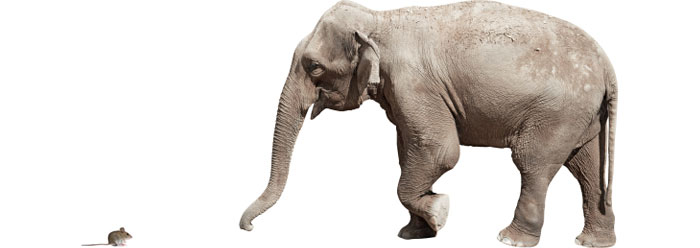
\includegraphics[width=8cm]{mouse_elephant.jpg}
	\end{center}

	\vspace{.5cm}
	\pause
	There are jobs that only these trucks can do. In order to be certain that these jobs get covered, we make sure that they are taken care of first.
\end{frame}


\section{High-Level Look}
\begin{frame}{Basically,}
\begin{enumerate}
	\item Receive data
\item Create optimal delivery/pickup pairs
\item For each driver:
	\begin{enumerate}
		\item Choose a transition to a nonempty zone (if they need a can, bring one)
			\begin{itemize}
				\item Special Truck: Go to a zone which has jobs requiring that truck.
			\end{itemize}
		\item Complete compatible jobs (satisfying truck size and time constraints) until the zone is depleted (choose another transition), or until driver's schedule is full.
			\begin{itemize}
				\item Special Truck: If dependent jobs in zone are depleted, transition to another zone that needs it.
			\end{itemize}
		\item Choose a transition to return to home base
	\end{enumerate}
\item Output schedule
\end{enumerate}
\end{frame}

\section{Results}
\begin{frame}{Teleportation}
	\begin{center}
	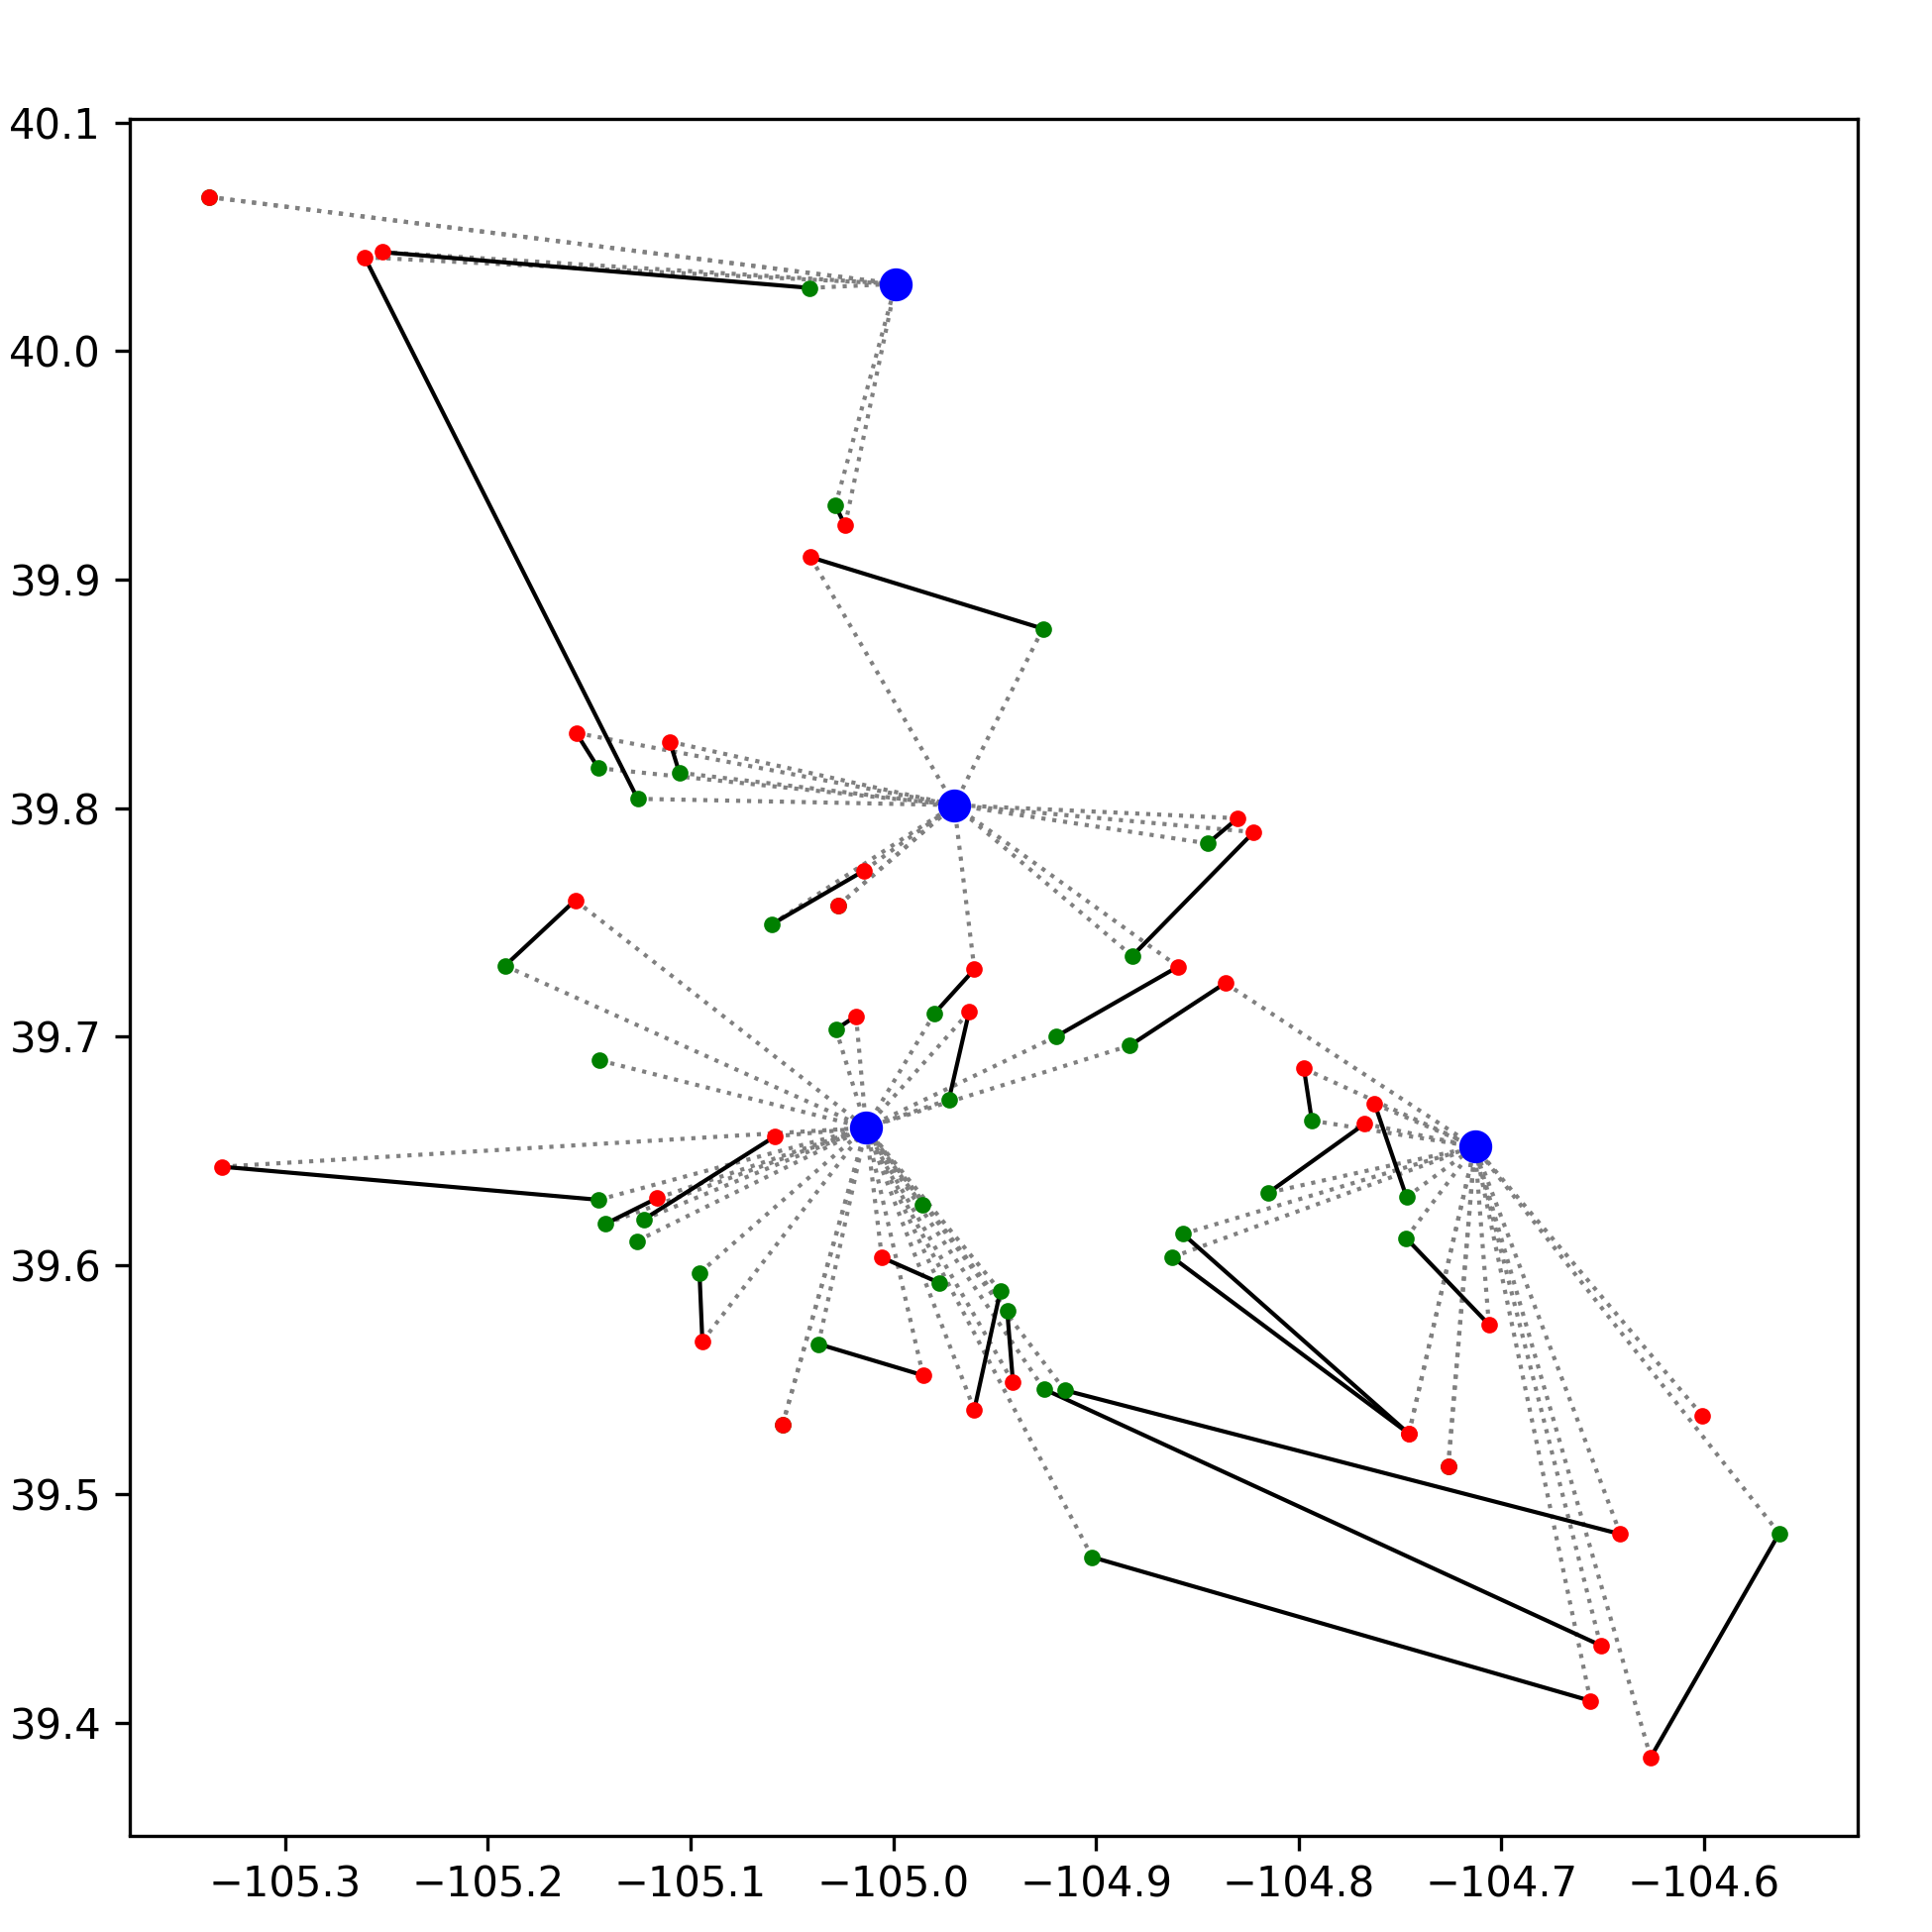
\includegraphics[width=7cm]{triangles.png}\\
	If drivers could teleport, 1534 minutes of driving.
	\end{center}
\end{frame}

\begin{frame}{Our Route, No Can Constraints}
	\begin{center}
	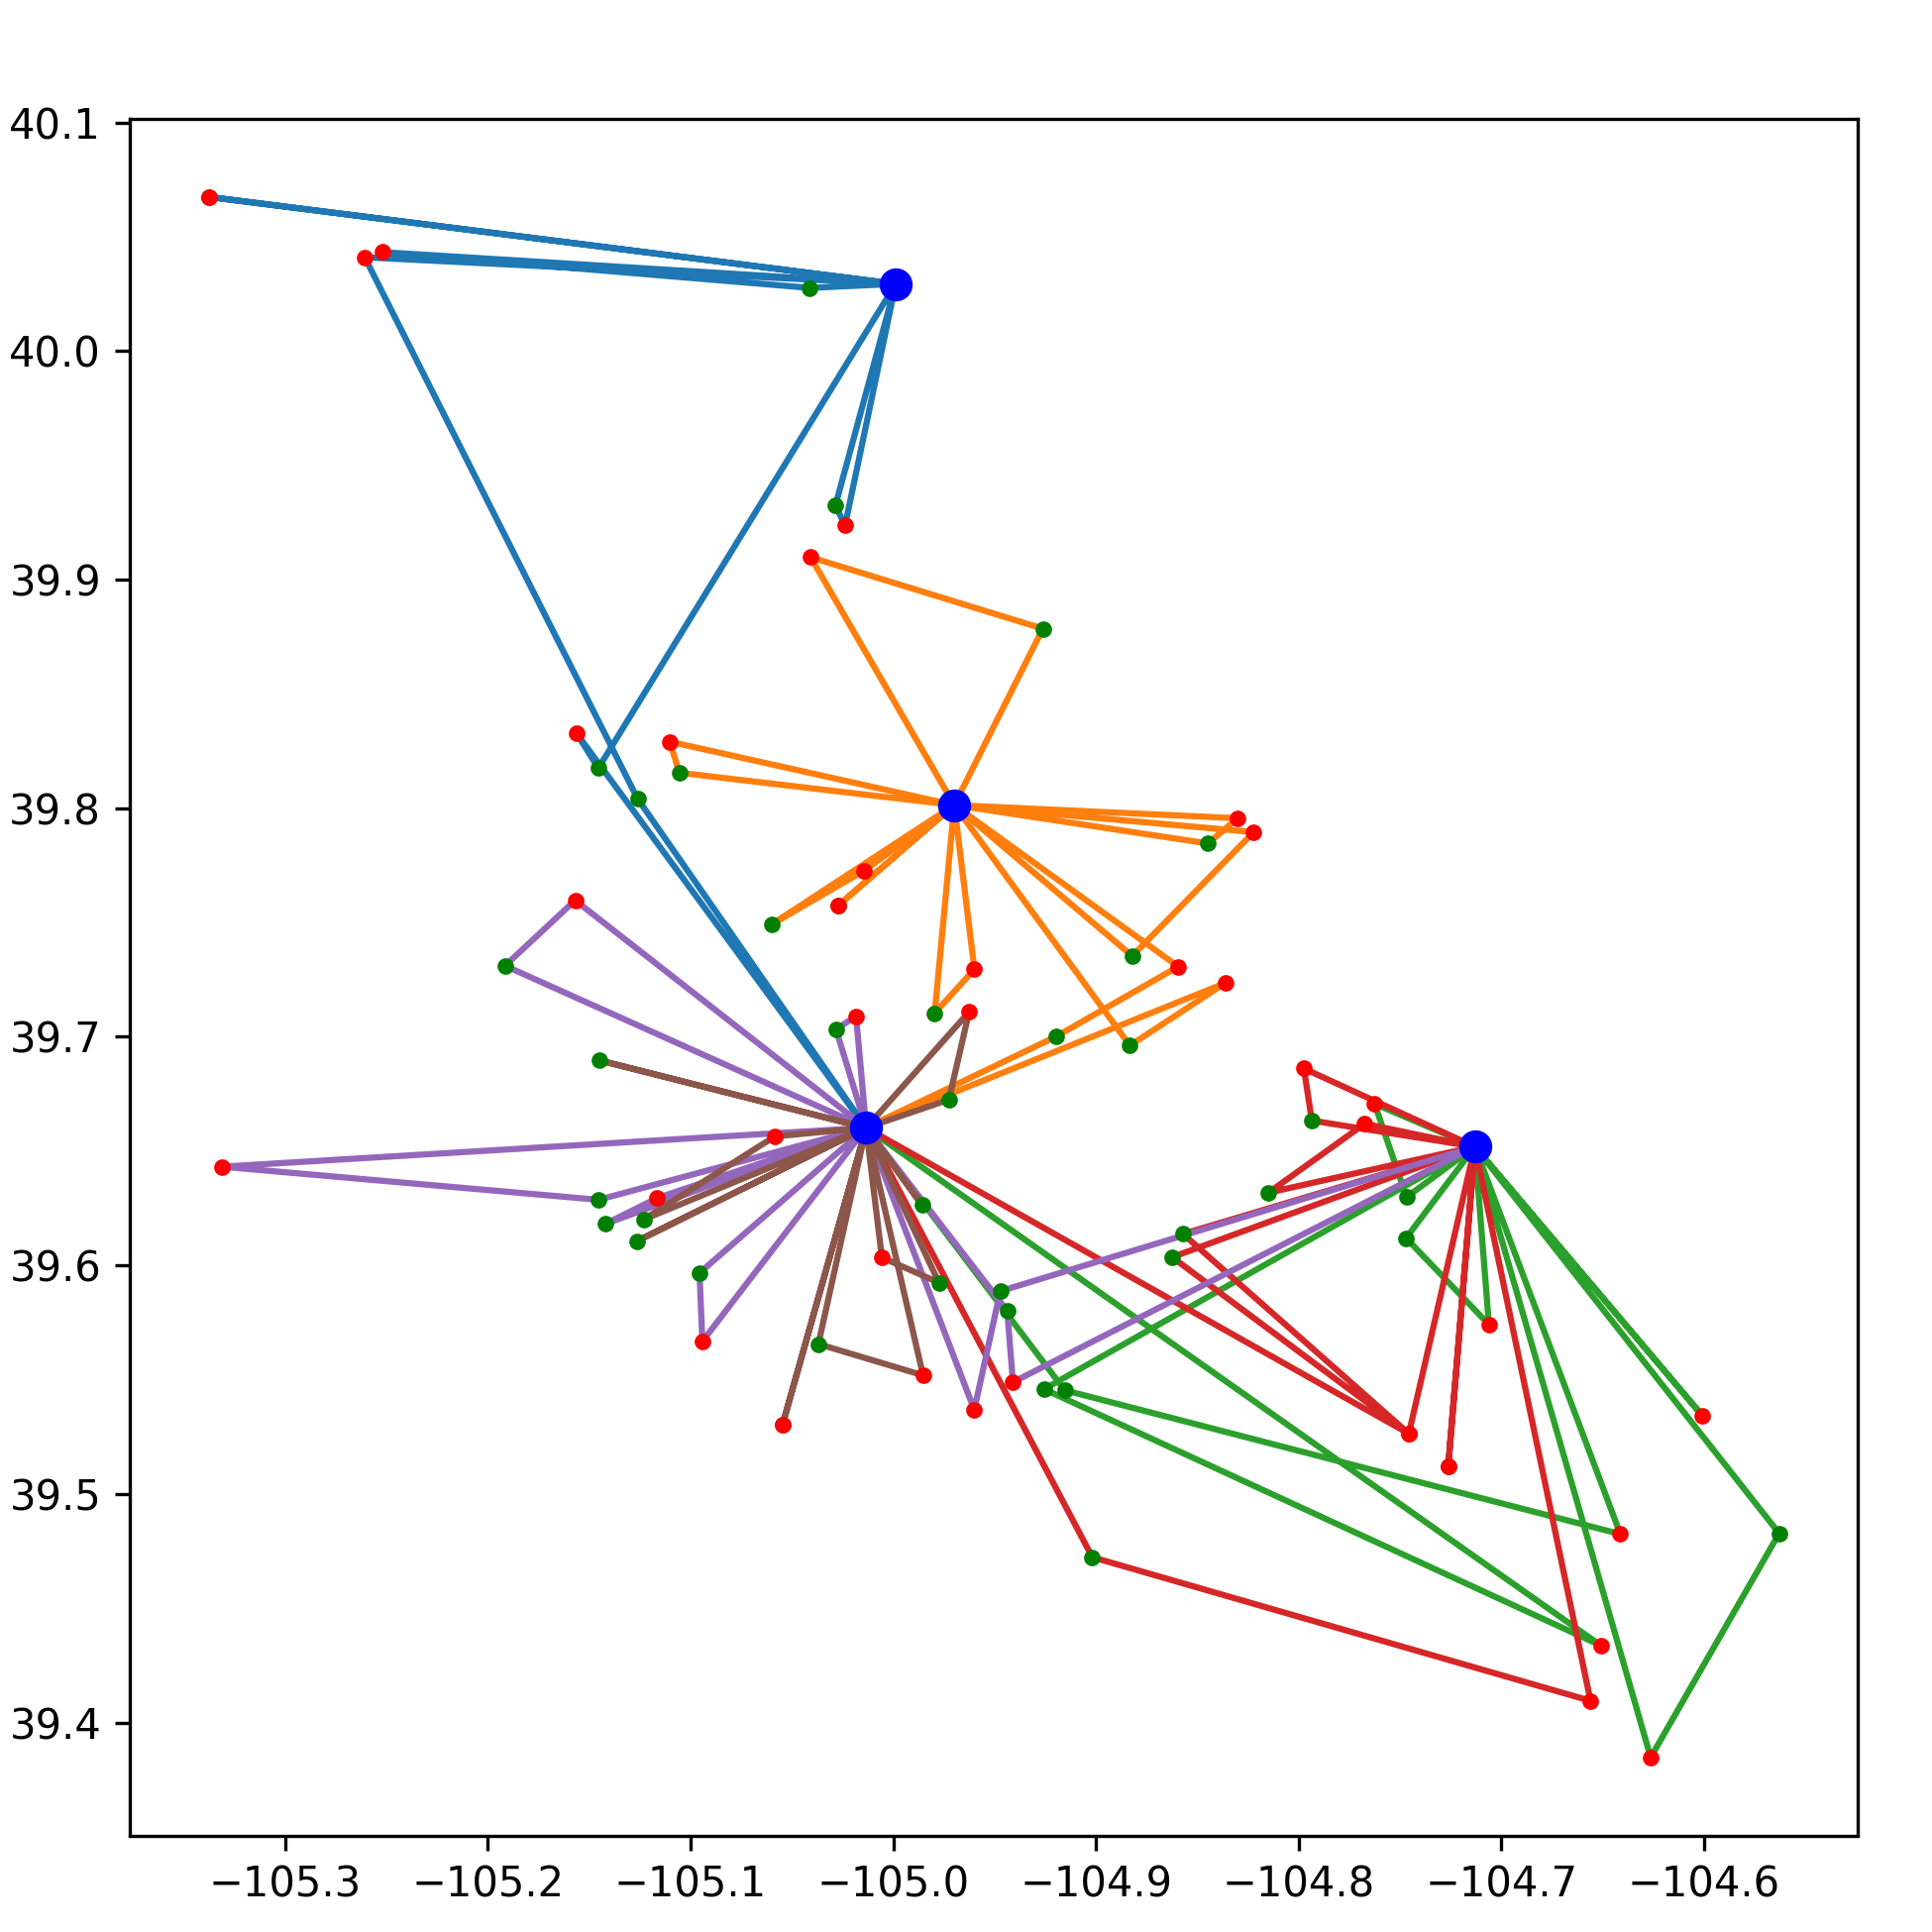
\includegraphics[width=7cm]{our_route.png}\\
	Our route, 1576 minutes of driving.
	\end{center}
\end{frame}

\begin{frame}{Our Route, Highly Restricted Cans}
	\begin{center}
	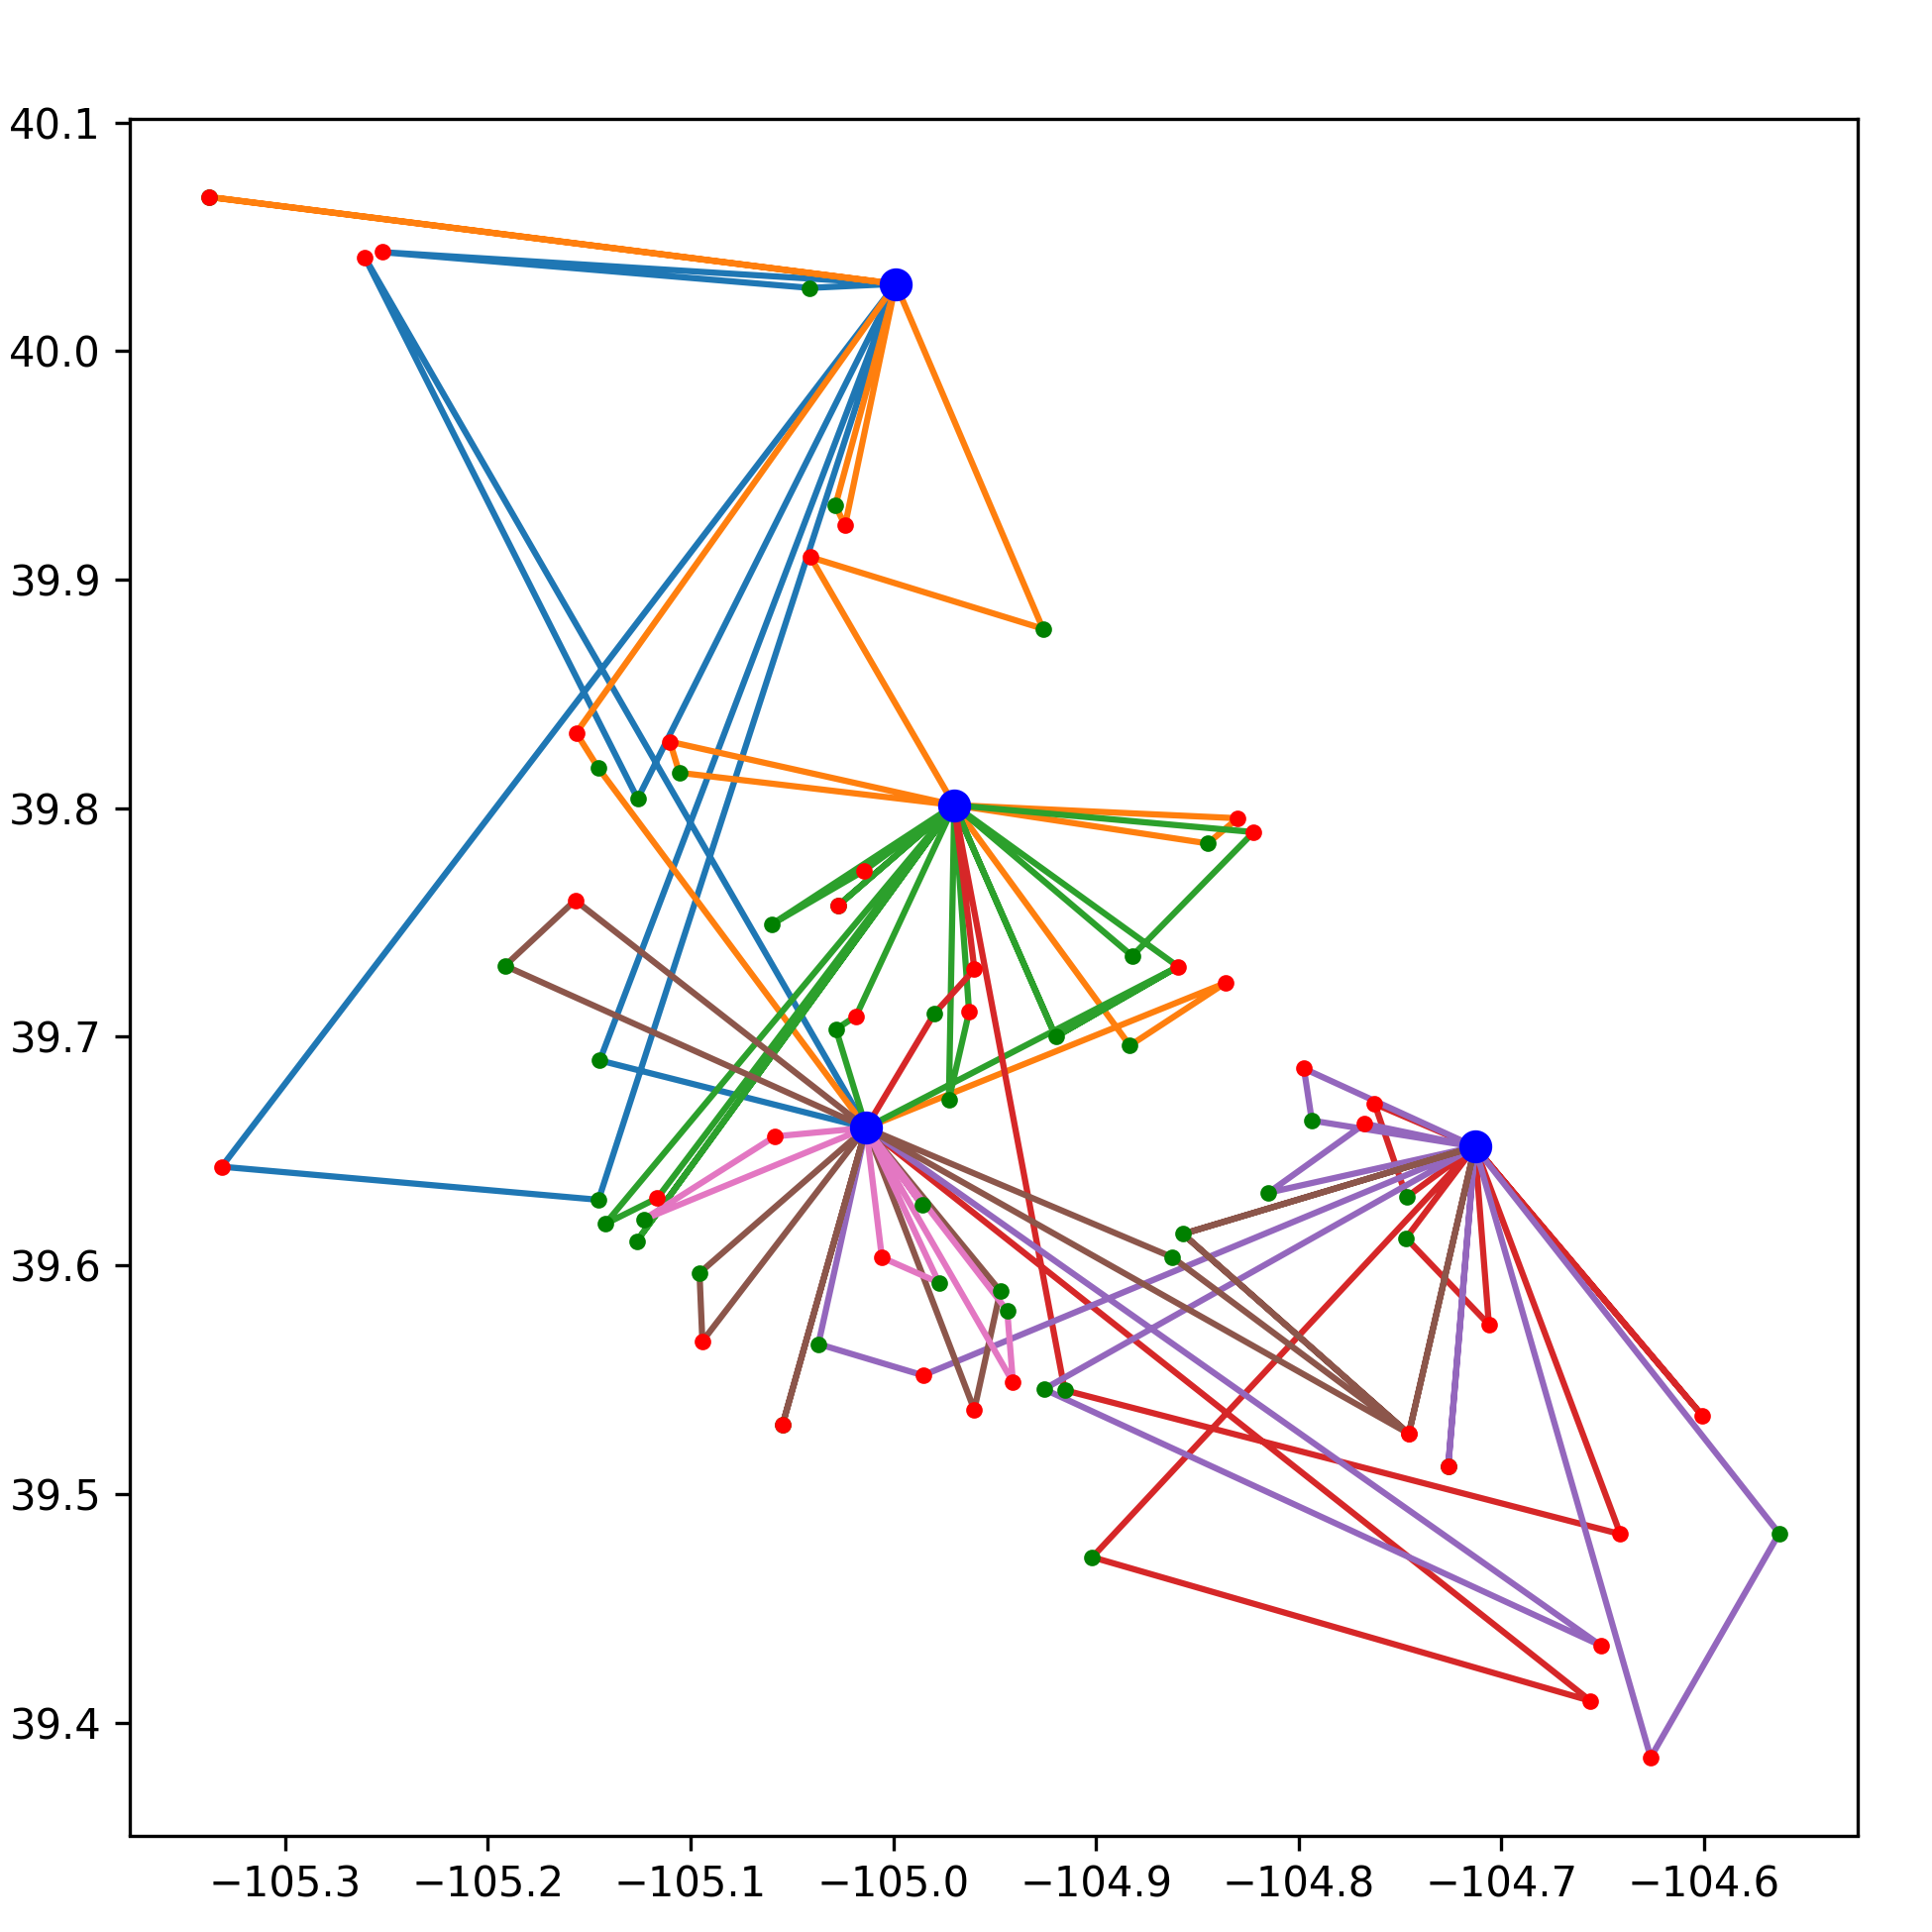
\includegraphics[width=7cm]{our_route_cans.png}\\
	Our route, 1781 minutes of driving.
	\end{center}
\end{frame}

\begin{frame}{Sam's Route}
	\begin{center}
	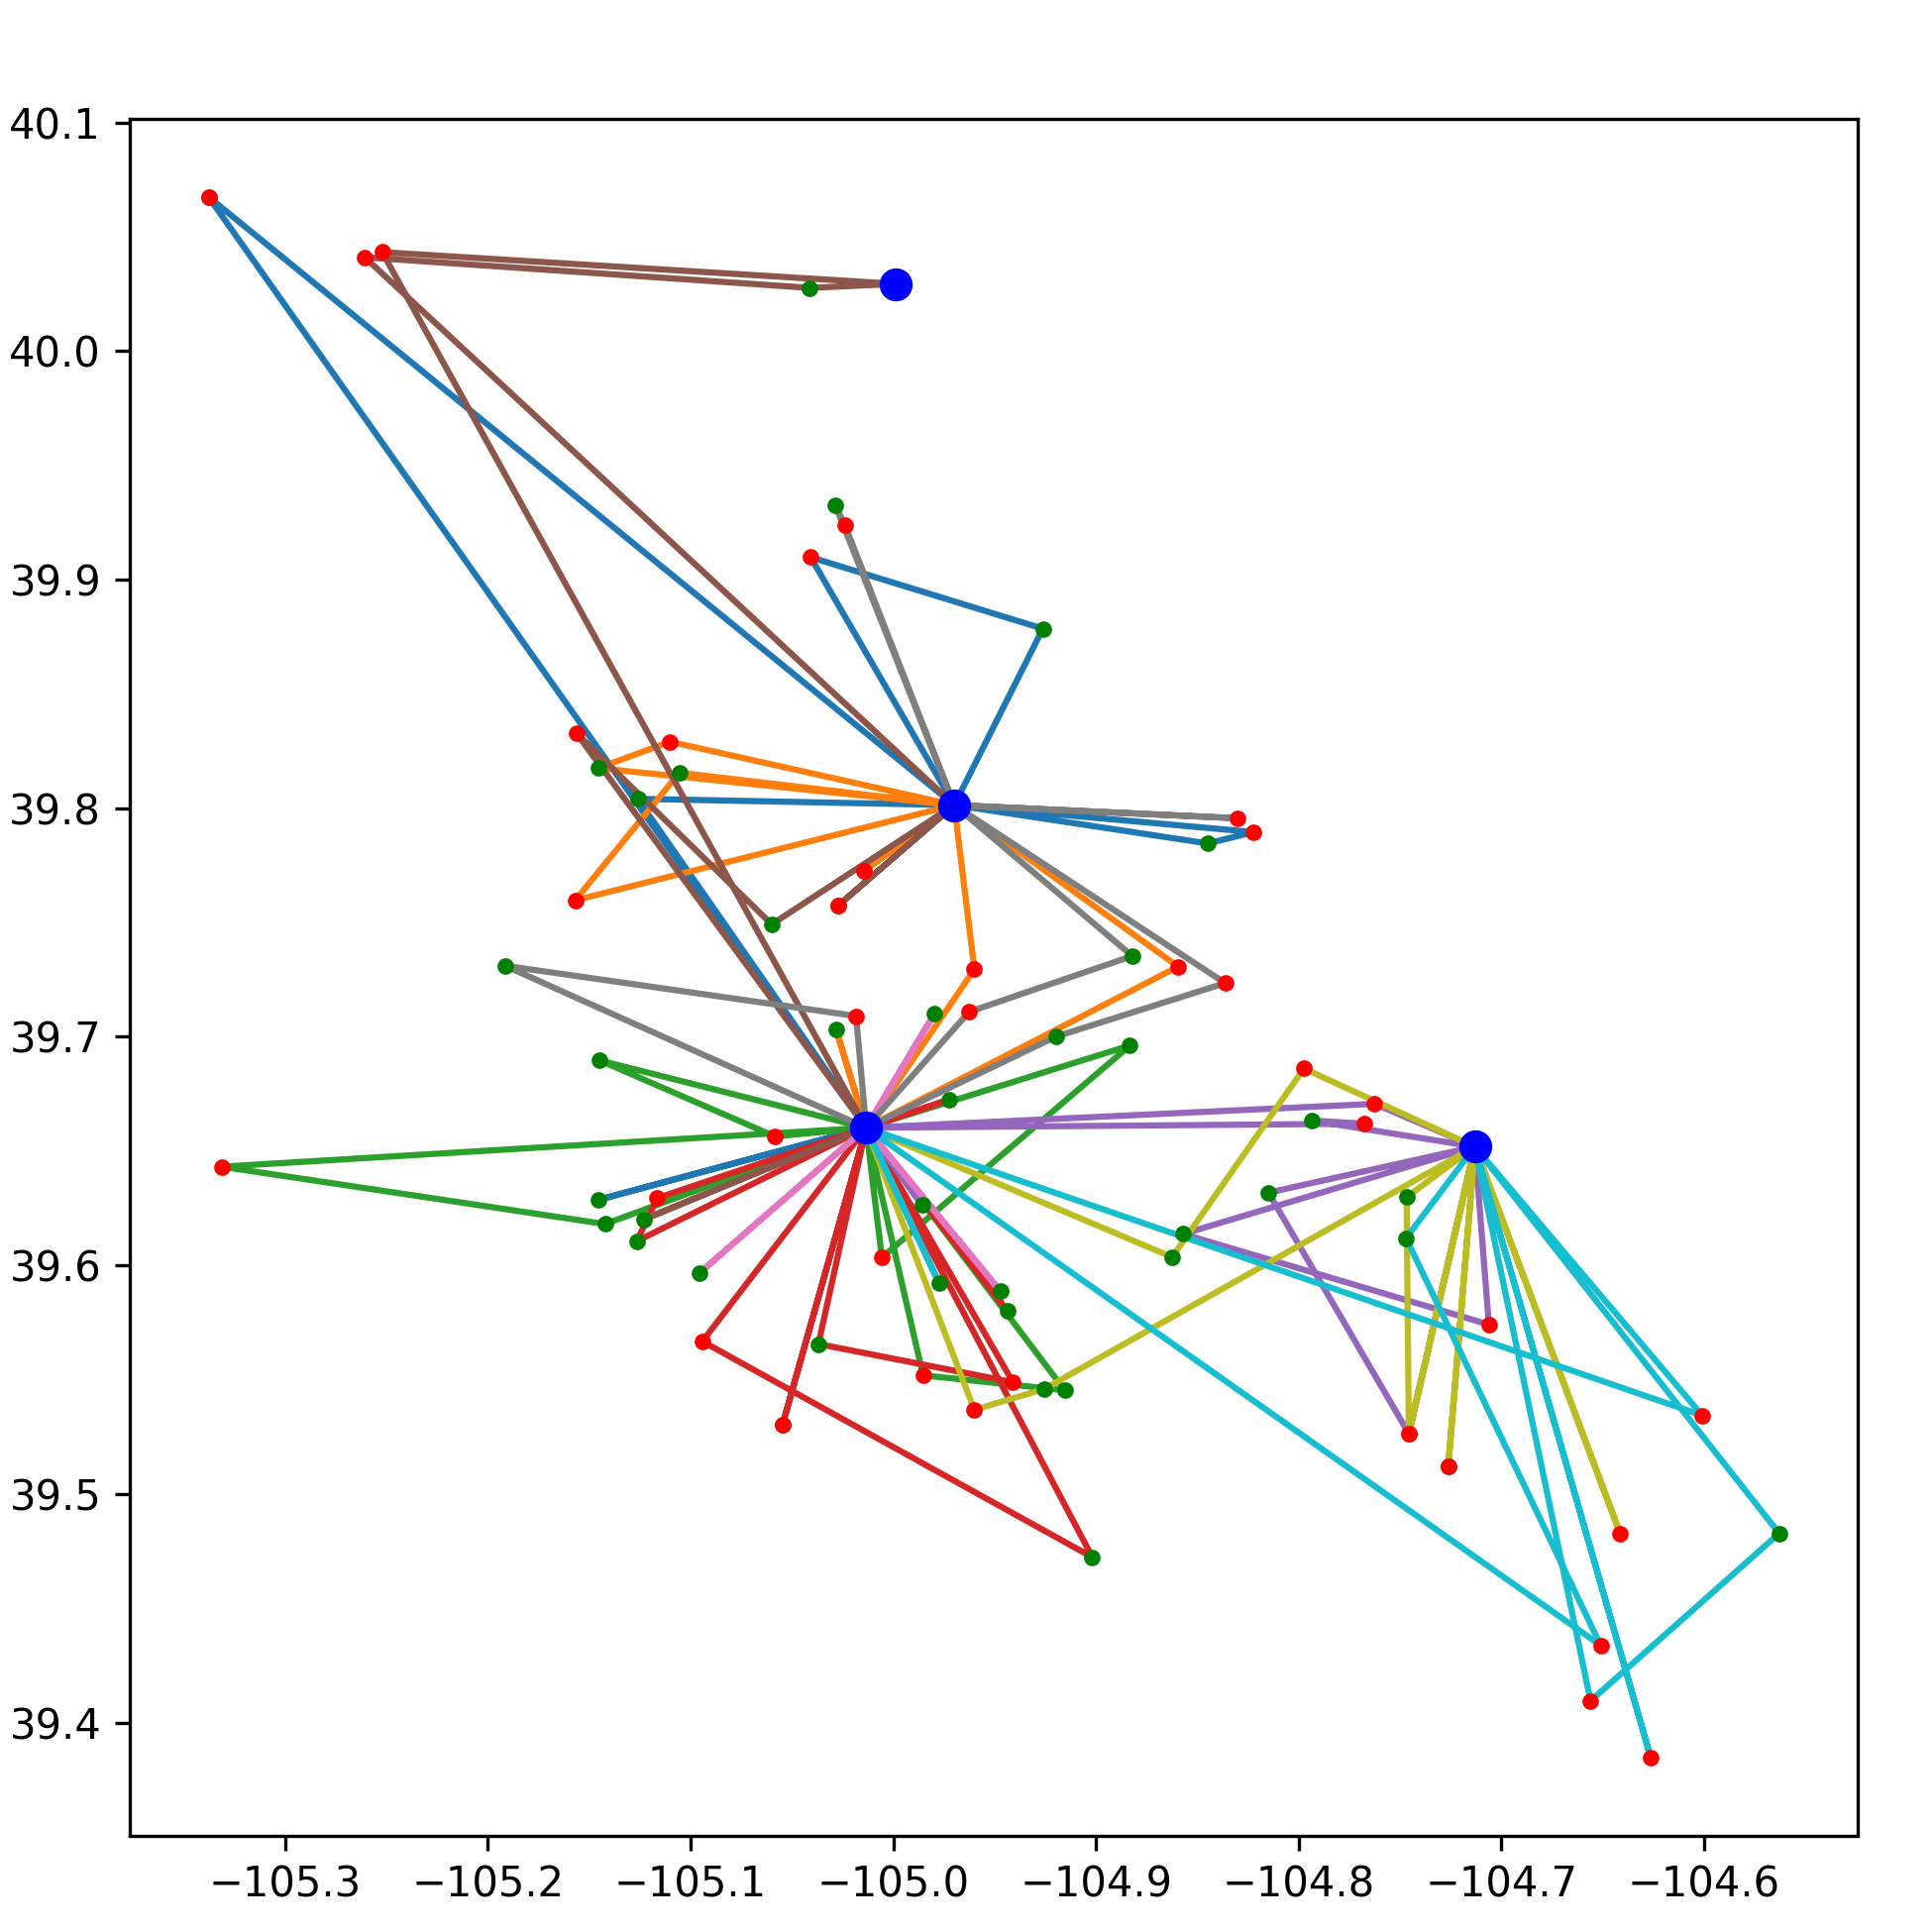
\includegraphics[width=7cm]{sams_route.png}\\
	Sam's Route, 1945 minutes of driving.
	\end{center}
\end{frame}

\begin{frame}{Comparison}
	\begin{center}
	\begin{tabular}{llll}
		Name & Minutes & $\%$ TP & $\%$ Sam's\\
		\hline
		Teleportation & 1534 & $0.0$ & $21.1$ \\
		No Can Constraints & 1576 & $2.7$ & $18.9$ \\
		Can Constraints & 1781 & $16.1$ & $8.4$\\
		Sam's & 1945 & $26.8$ & $0.0$\\
	\end{tabular}
	\end{center}
\end{frame}

\section{Conclusions/Future Work} 
\begin{frame}{Improvements}
	We are pleased with the outcome, the algorithm is quite fast and gives decent results. Though, there are some things which would make it better.
	\begin{itemize}
		\item Data (Driving Times)
		\item Data (Constraints)
		\item Better Pairs (?)
		\item Usability
	\end{itemize}
\end{frame}

\section*{}
\begin{frame}{What we covered}
\begin{multicols}{2}
	\tableofcontents
\end{multicols}
\end{frame}

\begin{frame}
\centering Thank You.
\end{frame}

\begin{frame}{References}

\end{frame}

\end{document}
